\documentclass[12pt]{ociamthesis}  % default square logo 
%\documentclass[12pt,beltcrest]{ociamthesis} % use old belt crest logo
%\documentclass[12pt,shieldcrest]{ociamthesis} % use older shield crest logo

%load any additional packages
\usepackage{amssymb}
\usepackage{amsmath,amsfonts,amsthm} % Math packages
%\usepackage[pdftex]{graphicx}
\usepackage[font=small,labelfont=bf, textfont=it]{caption}
\usepackage{subcaption}
\usepackage[style=numeric,sorting=none, backend=bibtex8]{biblatex} % used literature
\usepackage{siunitx}
\usepackage{hyperref}
\usepackage{placeins}
\usepackage{listings}
\usepackage{float}
\usepackage{wasysym}
\usepackage[sc]{mathpazo} % Use the Palatino font
\usepackage[T1]{fontenc} % Use 8-bit encoding that has 256 glyphs
\usepackage{microtype} % Slightly tweak font spacing for aesthetics
\usepackage[english]{babel} % Language hyphenation and typographical rules
%\usepackage[hmarginratio=1:1,top=32mm,columnsep=20pt, textwidth = 526pt]{geometry} % Document margins
\usepackage{booktabs} % Horizontal rules in tables
\usepackage{lettrine} % The lettrine is the first enlarged letter at the beginning of the text
\usepackage{enumitem} % Customized lists
\setlist[itemize]{noitemsep} % Make itemize lists more compact
\usepackage{hyperref} % For hyperlinks in the PDF


%input macros (i.e. write your own macros file called mymacros.tex 
%and uncomment the next line)
%\include{mymacros}

\title{Accessible Adaptive Optics and Super-resolution Microscopy to Enable Improved Imaging     %your thesis title,
}   %note \\[1ex] is a line break in the title

\author{Nicholas James Hall}             %your name
\college{Linacre College}  %your college

%\renewcommand{\submittedtext}{change the default text here if needed}
\degree{Doctor of Philosophy}     %the degree
\degreedate{Trinity 2020}         %the degree date

\bibliography{Reference_list}        %use a bibtex bibliography file Reference_list.bib

%end the preamble and start the document
\begin{document}

%this baselineskip gives sufficient line spacing for an examiner to easily
%markup the thesis with comments
\baselineskip=18pt plus1pt

%set the number of sectioning levels that get number and appear in the contents
\setcounter{secnumdepth}{3}
\setcounter{tocdepth}{3}


\maketitle                  % create a title page from the preamble info
\begin{dedication}
\textit{For everyone who cheered me on as I ran\\
but never got to see me cross the finish line;\\
Tell them I made it}
\end{dedication}        % include a dedication.tex file
\begin{acknowledgements}
	
	\vspace{-0.75cm}
	
	{\small %\begin{center}
		%\textit{No man is an island entire of itself, \\
		%	Every man is a piece of the continent,\\
		%	A part of the main.} - John Donne
		%\end{center}
		
		A particularly pernicious myth is that science is moved forward by 
		lone geniuses - this idea is just that, a myth. It would have been 
		impossible for me to get this far without an overwhelming amount of 
		support, a full account of which would likely be as long as the 
		thesis itself. Hopefully, this abbreviated form  will suffice.
		
		Firstly, I would like to thank my supervisors; Ian Dobbie, Martin 
		Booth and Ilan Davis. Their input, feedback, expertise, and 
		encouragement were invaluable to me. Ian in particular was always 
		on hand to offer support and insight at critical moments. I owe 
		everyone I worked alongside at Micron during my time a debt of 
		gratitude, particularly Mick Philips and David Pinto; building and 
		writing code for bespoke super-resolution microscopes has one hell 
		of a learning curve, and you made it much easier for me to climb 
		it. Thank you for showing me the ropes, answering my many questions 
		and for tolerating my more vocal outbursts in the office when 
		Python proved particularly adversarial. 
		
		I received incredible support from the Davis lab, particularly from Richard Parton, Josh Titlow and Dalia Sara Gala in providing biological 
		samples and key feedback. From the Dynamic Optics and Photonics 
		Group, I am extremely grateful to Mantas \v{Z}urauskas, Jacopo 
		Antonello and Syed Hussain for their expertise and advice on 
		adaptive optics. It has been my immense pleasure to learn from and 
		work alongside such accomplished individuals. 
		
		My thanks to Sara Abrahamsson and Marcel M\"{u}ller for their encouragement and willingness to collaborate with me on a number of occasions. 
		
		The 2016 ONBI cohort, program coordinator Peter Jezzard, and 
		administrator Lisa Bligh all deserve thanks for building a 
		supportive environment to enjoy camaraderie, laughter, and many, 
		many caterpillar cakes.
		
		Rick Lange, Sarah Fynes-Clinton, Barney Bridges, Leah Barton, 
		John-Luke Treadgold, Simon Parnham, Jon Collins, Tim Curtis, and 
		Kyle Hall have all given me unflagging support, encouragement, and 
		enthusiasm. They have been boundless sources of joy, levity, and 
		steadfast bulwarks when I needed them most. I will never forget 
		their faultless kindness to me. If a man's wealth is indeed 
		measured by his friendships, I am rich beyond all measure.
		
		Finally, I would like to thank my family: my parents, Trevor and 
		Karen Hall; my sister and brother-in-law, Annabelle and Christopher 
		Holloway; and my sister, Meghan Hall. They have consistently been 
		my most vocal supporters, and fierce sources of love and 
		encouragement. The fruits of my labour are a testament to the good
		soil I was planted in and the nourishment I received from them.
		
		You all have my eternal gratitude and my most heartfelt, effusive 
		thanks.}
	
\end{acknowledgements}   % include an acknowledgements.tex file
\begin{abstract}
	
	Many of the recent innovations in biological imaging have revolved around the 
	quest for greater resolving power, ultimately culminating in the advent of
	super-resolution microscopy techniques. However, all microscopy techniques are
	vulnerable to optical aberrations which distort the light wavefront. This leads 
	to a gulf between theoretical and practical resolution for an imaging system. 
	For super-resolution techniques, this can lead to reconstruction artifacts or 
	the failure of the imaging technique entirely.
	
	Implementing adaptive optics (AO) in microscopy has already been shown to be 
	highly effective at reducing  these aberrations and yielding significant 
	improvements to image quality and resolution in numerous proof of principle 
	systems. Despite this, AO technology has yet to be widely adopted in 
	microscopy. This is for two principle reasons. Firstly, AO implementations to 
	date have not been robust or generalised which makes transferring them between 
	microscopy systems, imaging modalities and sample type troublesome to 
	impossible. Secondly, AO implementations to date have not been accessible to 
	typical microscope users and instead have been the purview of AO microscopy 
	specialists.
	
	This thesis presents a generalised, robust implementation for AO; 
	Microscope-AOtools. This implementation has all the necessary methods for 
	setting up and operating an adaptive element in microscopy. It has a flexible, 
	modular design which allows for easy transfer between imaging systems, 
	modalities, hardware configurations and sample types. These methods are 
	integrated into Microscope-Cockpit for user accessibility. The evidence of 
	these claims are substantiated by a detailed description of Microscope-AOtools' 
	successful deployment on both a spinning disk confocal system and a bespoke, 
	upright structured illumination microscope with a range of sample types.
	
\end{abstract}
          % include the abstract

\begin{romanpages}          % start roman page numbering
\tableofcontents            % generate and include a table of contents
\listoffigures              % generate and include a list of figures
\end{romanpages}            % end roman page numbering

%now include the files of latex for each of the chapters etc
\chapter{Introduction}

\section{Introduction to Microscopy}
\label{sec:microscopy}

The principle of optical magnification was known at least as early as the 1st 
Century CE. The enhancement of resolving power for objects viewed through 
spherical glass objects filled with water (a kind of proto-lens) was noted by 
Seneca and some of his contemporaries\cite{seneca1971naturales}. Even after 
the collapse of the Roman Empire and Europe entered the Dark Ages other 
scholars, such as Ibn al-Haytham, noted and investigated the phenomenon of 
optical magnification through convex-planar pieces of 
glass\cite{nasr1968science}. Given the importance which microscopy has had in 
furthering biological understanding, it is an amusing anecdote that it took 
over a millennia for anyone to identify an application for the phenomenon of 
magnification. It was not until the end of 13th Century  when Roger Bacon 
penned his \textit{Opus majus} that a practical use for magnification could 
be found - eyeglasses. It was a further 300 years until the first telescopes 
and microscopes were developed. The exact date and inventor of the first 
telescope is unknown, but the credit is usually attributed to one of four 
Dutchmen at the start of the 17th Century; Hans Janssen, his son Zacharias, 
Hans Lippershey, or Jacob Metius. Likewise, precise date and inventor of the 
first microscope is not known, but the invention did occur at around the same 
time and the term was coined by Giovanni Faber in 
1625\cite{bardell2004invention}. It is interesting to note that the invention 
of microscopes and telescopes are so closely linked, and that both astronomy 
and microscopy continued enjoy a mutually beneficial relationship. The true 
power of microscopes to yield novel biological understanding was first 
popularised by Robert Hooke and then later by Antonie van 
Leeuwenhoek\cite{hooke1665micrographia, chung2017pioneers}. Since then, the 
microscope has been and remains one of the premiere tools enabling biological 
discoveries.

\subsection{Fluorescence microscopy}
\label{subsec:fluorescence}

Microscopes allowed biologists to visualise structures well below the 
length-scale available to the naked eye. However, living material still 
remained resistant to optical examination due to a number of properties: 
strong scattering properties, particularly for wavelengths of light 
within the visible spectrum; transparency; innate light-protective 
mechanisms to prevent damage from solar radiation. Phase contrast 
microscopy could solve some of the issues when visualising otherwise 
transparent samples\cite{burch1942phase}. More typically microscopy 
samples were chemically fixed as these samples were more stable and 
easier to refractive index match to the microscope. Histological staining 
was, for decades, the primary method for revealing biological structures\cite{alturkistani2016histological}. The properties and function 
of living material were then inferred from fixed samples. This was, as one 
author put it, ``like reconstructing a football game from a series of still 
pictures,...an arduous (and some would say hopeless) 
endeavour''\cite{yuste2005fluorescence}. 

Fluorescence microscopy enabled the selective visualisation of specific 
molecules, as well as the imaging of dynamic processes \textit{in situ}. 
Fluorescence is the property of atoms and molecules whereby they emit light
after stimulation from an external energy source. In steady-state conditions 
(i.e. without an external energy source) the electrons of the atom or  
molecule are found in the ground state. Photons from the external energy  
source are absorbed by these electrons, raising them to excited singlet 
states. When these excited electrons return to the ground state, they can 
release their energy as a photon - it is this phenomenon which is called 
fluorescence\cite{ghiran2011introduction}. For atoms, these energy states are
reasonably discrete and (for the lowest levels) easy enough to draw in 
Jab\l{}onski diagrams. Molecules capable of fluorescence, called 
fluorophores, have broad ``energy bands'' of possible excitation and emission 
wavelengths. Additionally, the absorption and emission cross-sections are not 
the same for all wavelengths. This leads to excitation and emission spectra 
for fluorescent molecules. Figure~\ref{fig:GFP_emission_absorption_spectra} 
shows the excitation and emission spectra for Green Fluorescent Protein 
(GFP), generated with SpekCheck\cite{phillips2018spekcheck}.

\begin{sidewaysfigure*}
	\centering
	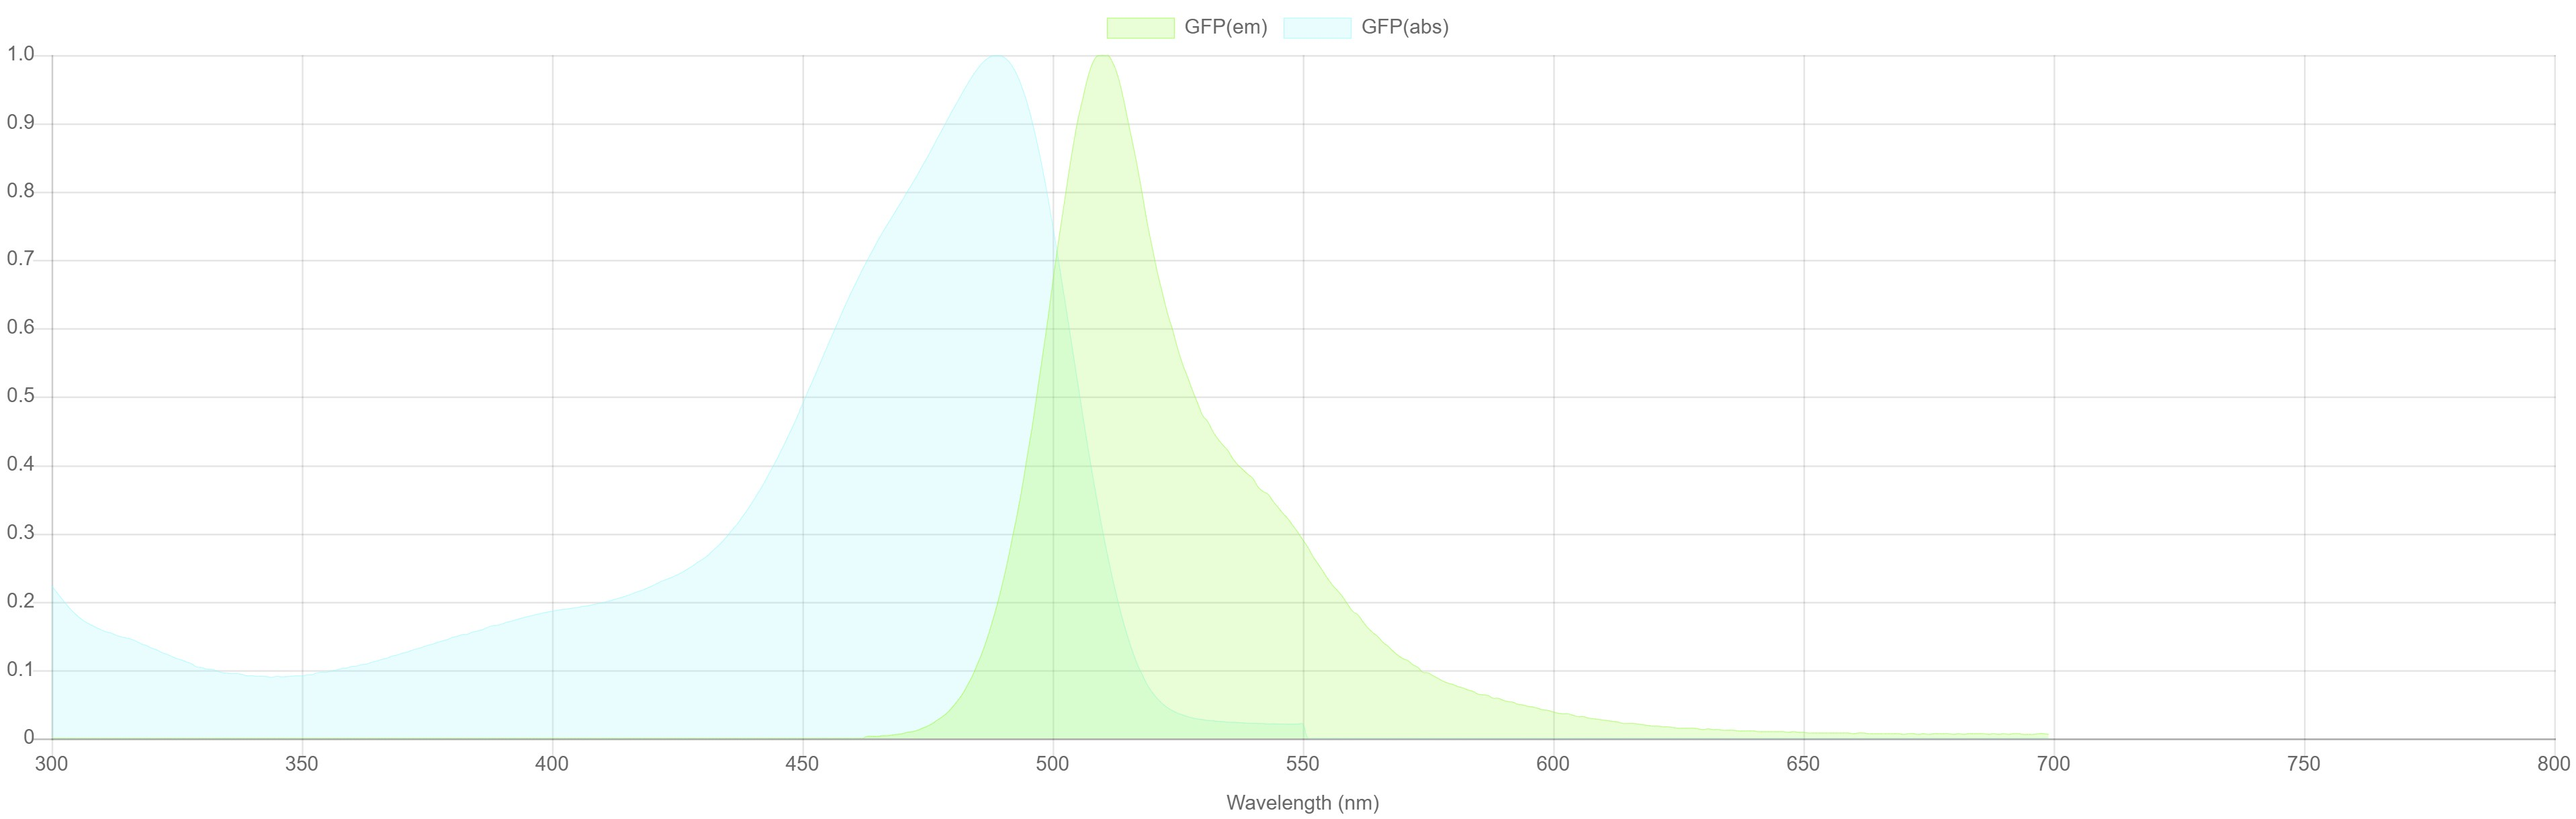
\includegraphics[width=\textwidth]{images/GFP_emission_absorption_spectra.jpg}
	\caption[Example excitation and emission spectra]{Example excitation (blue) 
		and emission (green) spectra for Green Fluorescent Protein. Generated with SpekCheck\cite{phillips2018spekcheck}}
	\label{fig:GFP_emission_absorption_spectra}
\end{sidewaysfigure*}

The first fluorescence microscopes were developed at the beginning of the 20th Century\cite{yuste2005fluorescence,renz2013fluorescence}. The real power of 
fluorescence microscopy came as the specificity of labelling improved. The 
first iteration of this was the development of antibody fluorescent labelling 
which allowed for, among other things, localisation of viral particles in 
biological 
cultures\cite{coons1942demonstration,coons1951fluorescent,weller1954fluorescent}.
The second, and arguably more profound, iteration was the discovery and 
cloning of \textit{Aequorea Victoria} GFP, and the development of chromatic
variants\cite{prasher1992primary,heim1996engineering}. This allowed for 
specific proteins of interest to be individually labelled and for biologists 
to monitor gene-expression\cite{chalfie1994green}. Since then, additional 
properties of fluorescent proteins, such as their conformational changes 
in response to binding events, environmental changes, or enzymatic activity, 
have been utilised to great effect\cite{toseland2013fluorescent}. 
Fluorescence microscopy has allowed biologists to visualise dynamic biological
processes in real time.

\subsection{Resolution}
\label{subsec:resolution}

A fundamental property of all microscopes and microscopy images is that of 
resolution - the minimum separation between two objects where they can still
be determined to be two distinct objects. Consider an optical plane, 
$\textbf{O}$, where a biological specimen is placed - the `sample plane'. Also
consider a separate optical plane, $\textbf{O'}$, where the image of the
specimen is formed - the `image plane'. The microscope, with circular entrance
and exit pupils, maps the field distributions between $\textbf{O}$ and 
$\textbf{O'}$. Figure~\ref{fig:simplified_microscope_layout} shows a schematic
of this simplified system.

\begin{figure}[h]
	\centering
	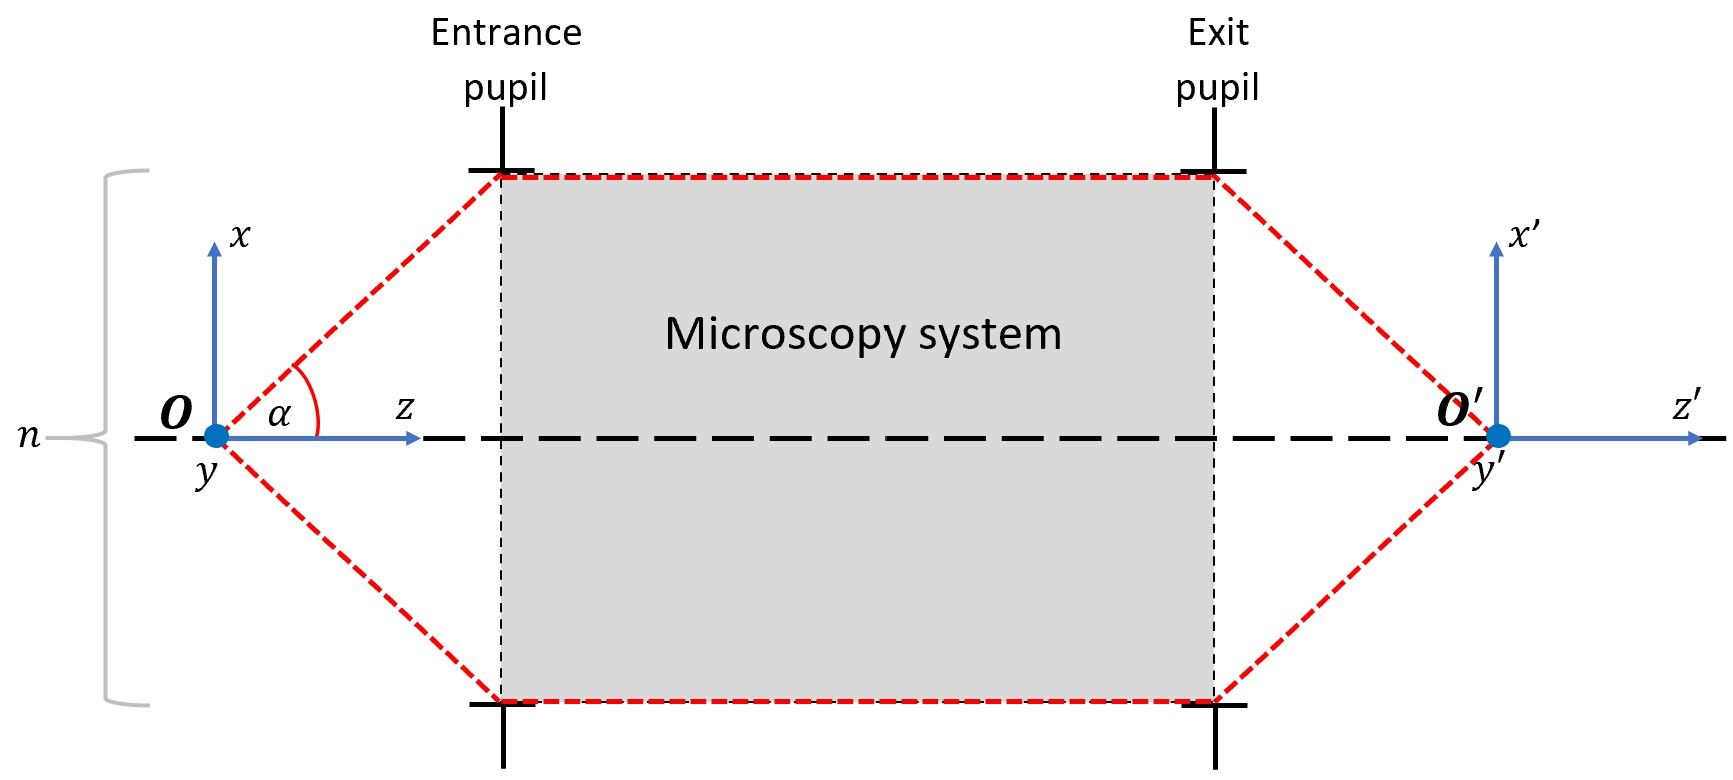
\includegraphics[width=\textwidth]{images/simplified_microscope_layout.jpg}
	\caption[A simplified schematic of a light microscope.]{A simplified 
		schematic of a light microscope. A specimen 
		is placed at the sample plane, $\textbf{O}$, in refractive index, $n$. Light 
		rays emerging from $\textbf{O}$ are collected by the entrance pupil. These 
		rays process through the microscope system before emerging at the exit pupil 
		and being focused at the image plane, $\textbf{O'}$. The light rays which 
		form and angle with the optical axis, $\textbf{OO'}$, of $\alpha$ are called
		marginal rays. Marginal rays are the highest diffraction order collectable by
		the entrance pupil and therefore the microscope system as a whole.}
	\label{fig:simplified_microscope_layout}
\end{figure}

Consider a point source located at $\textbf{O}$ isotopically emitting 
monochromatic light of wavelength $\lambda$. Every ray forms an angle, 
$\theta$, with the optical axis $\textbf{OO'}$. The highest angle collected
by the entrance pupil is $\alpha$. A point source can be considered an 
infinitely narrow aperture and $\alpha$ determines the highest 
diffraction order which the entrance pupil - i.e. the microscope
objective aperture - can collect\cite{davidson2002optical}. Considering this 
and, more generally, the diffraction of light through a circular aperture 
it is possible to obtain that the field intensity at \textbf{O'} is 
proportional to\cite{goodman2005introduction,born2013principles}:

\begin{equation}\label{eq:image_field_insentity}
\mathcal{I}_{w}(v) = \left|\frac{2\mathcal{J}_{1}(v)}{v}\right|^2,
\end{equation}

where $\mathcal{J}_{1}(v)$ is the first-order Bessel function of the first 
kind of the variable $v$\cite{watson1995treatise}. $v$ is the normalised 
lateral co-ordinate given by\cite{wilson1984theory}:

\begin{equation}\label{eq:normalised_lateral}
v = \frac{2\pi}{\lambda}rn\sin(\alpha).
\end{equation}

$r$ is the radial displacement in the image plane $\textbf{O'}$, $r = \sqrt{x'^{2} + y'^{2}}$. 
A useful quantity, and one often cited by microscope objective manufacturers, 
is the numerical aperture, $NA = n\sin(\alpha)$. The Rayleigh criterion 
determines that the limit at which two point objects can be meaningfully 
separated is when the central maxima of one diffraction pattern lies in the
first minimal of the other\cite{rayleigh1874xii,rayleigh1880investigations}. For a first order Bessel 
function, this occurs at $v \approx 1.22\pi$. Therefore, the lateral resolution 
limit, $r_l$ is often quoted as:

\begin{equation}\label{eq:lateral_res}
r_l \approx \frac{1.22\lambda}{2NA}
\end{equation}

otherwise known as the Abbe diffraction limit\cite{abbe1873beitrage}. Through
a similar process and considering the field intensity along the $z'$ axis, the
axial resolution, $r_a$, is given as\cite{pawley2006handbook}:

\begin{equation}\label{eq:axial_res}
r_a \approx \frac{2\lambda n}{NA^{2}}.
\end{equation}

Figure~\ref{fig:Airy_ring_2_object_seperation} shows two 
diffraction-limited point objects at variable lateral separations. For 
lateral separations less than $r_{l}$ the field intensities resemble a single 
point source in the image plane. For lateral separation at or above $r_{l}$ 
the intensity contributions from the two objects are distinguishable as 
separate.

\begin{figure}[h]
	\centering
	\begin{subfigure}{0.49\textwidth}
		\centering
		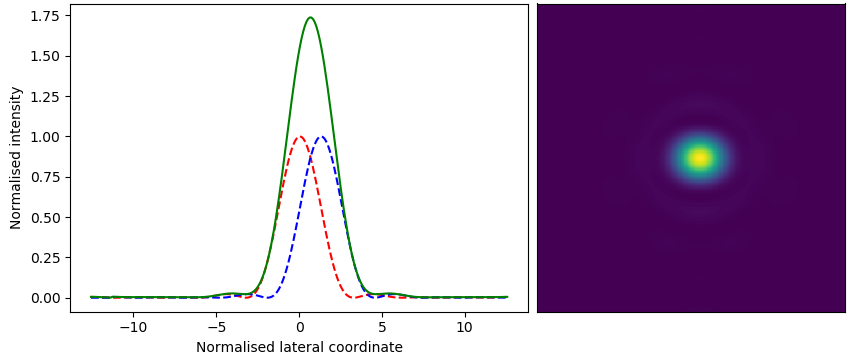
\includegraphics[width=\linewidth]{images/Airy_ring_2_object_seperation_0_5.png}
		\caption{Object separation = $0.41\text{r}_{\text{l}}$}
		\label{fig:Airy_ring_2_object_seperation_0_5}
	\end{subfigure}
	\begin{subfigure}{0.49\textwidth}
		\centering
		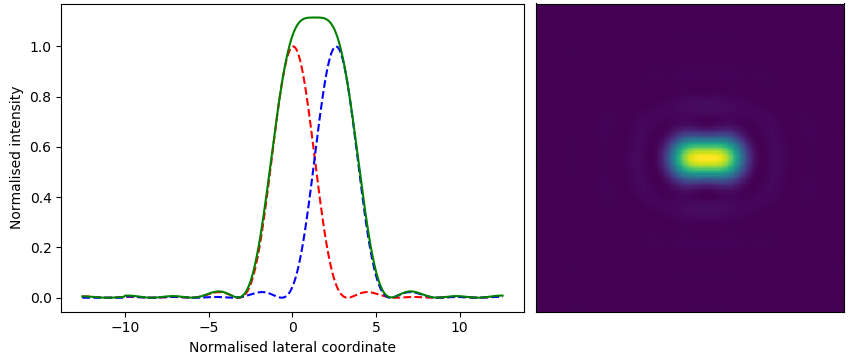
\includegraphics[width=\linewidth]{images/Airy_ring_2_object_seperation_1_0.png}
		\caption{Object separation = $0.82\text{r}_{\text{l}}$}
		\label{fig:Airy_ring_2_object_seperation_1_0}
	\end{subfigure}
	\begin{subfigure}{0.49\textwidth}
		\centering
		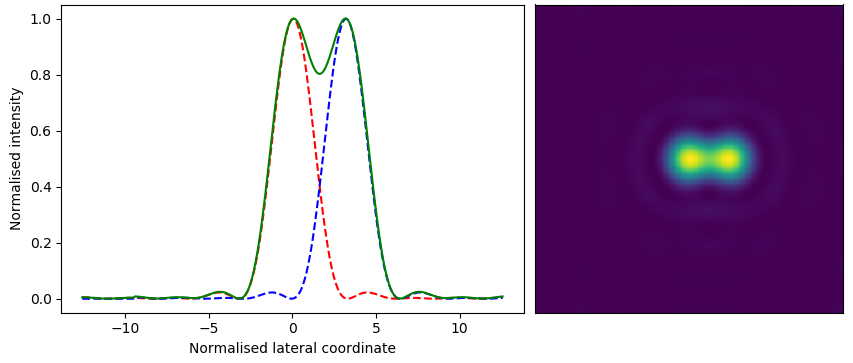
\includegraphics[width=\linewidth]{images/Airy_ring_2_object_seperation_1_22.png}
		\caption{Object separation = $1.0\text{r}_{\text{l}}$}
		\label{fig:Airy_ring_2_object_seperation_1_22}
	\end{subfigure}
	\begin{subfigure}{0.49\textwidth}
		\centering
		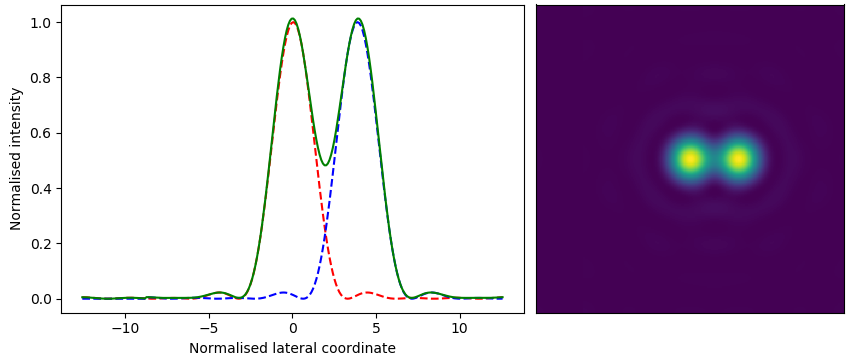
\includegraphics[width=\linewidth]{images/Airy_ring_2_object_seperation_1_5.png}
		\caption{Object separation = $1.23\text{r}_{\text{l}}$}
		\label{fig:Airy_ring_2_object_seperation_1_5}
	\end{subfigure}
	\caption[Illustration of the resolution limit as determined by the Rayleigh
	criterion]{Illustration of the resolution limit as determined by the Rayleigh 
		criterion. Each subfigure shows a line profile and 2D plot of the field 
		intensity distributions of both of the two diffraction limited point 
		objects. For two point objects separated by $< r_{l}$, \textbf{(a)} \& 
		\textbf{(b)}, they are not separable as individual objects. At a 
		separation $\ge r_{l}$, \textbf{(c)} \& \textbf{(d)}, the two point 
		objects are separable.}
	\label{fig:Airy_ring_2_object_seperation}
\end{figure}

Several approximations had to be made to obtain Equations~\ref{eq:lateral_res}
and~\ref{eq:axial_res}. Firstly, the Fraunhofer and paraxial approximations are
assumed to hold\cite{goodman2005introduction}. Obviously, the microscope system
has been greatly simplified to essentially just the entrance and exit pupils. 
More complex but accurate models for modern microscopy set-ups have been 
demonstrated\cite{torok2007optical, foreman2011computational}. Finally, this
idealised system only considers the shape of the apertures - i.e. the entrance
and exit pupils - and the wavelength of light. If one were to observe objects 
such as these, with these field distributions corresponding to well-specified
models, there would be no resolution limit at all\cite{den1997resolution}. In 
practice, the field distributions of objects are not precisely known, therefore
determining the location of the first minima is not as simple as it has been 
presented here. The first minima may not even be radially symmetric. 

Furthermore, the `true' resolution achievable by a microscopy system is 
affected by other factors such as the signal-to-noise ratio of an image, 
coherence conditions of illumination, apodization, discretisation errors for 
digital cameras, to name a few\cite{den1997resolution}. There have been 
attempts to develop alternative resolution measurements for point 
objects\cite{ram2006beyond}. Unfortunately, the actual resolution achieved in 
biological samples varies across the image plane, determined by factors such 
as the labelling density of the underlying biological 
specimen\cite{culley2017nanoj}. The `true' resolution of a system for a given 
sample is therefore a quantity which is impossible to determine analytically. 
The ideal lateral and axial resolutions in Equations~\ref{eq:lateral_res} 
and~\ref{eq:axial_res} are nonetheless useful quantities as the theoretical, 
ideal resolution limit of a microscopy system.

Returning to the concept of a point object as an infinitely narrow aperture allows 
for a more complete understanding of the resolution limit. A spatially structured 
object can be described by a superposition of spatial frequencies in the same 
manner in which a temporally structured object can be described by a superposition 
of temporal frequencies, which is the basis for Fourier 
optics\cite{goodman2005introduction}. A point object can be described as a Dirac
delta function, the Fourier transform of which is a uniform distribution across all
spatial frequencies. The addition of an aperture, such as a microscope objective, 
effectively imposes a low-pass filter on the spatial frequency domain. 
Figure~\ref{fig:WF_OTF} shows the projection of the observable region onto the 
lateral spatial frequency plane $k_{x}k_{y}$ i.e. the low-pass filter. The radius of
this low-pass filter is: 

\begin{equation}\label{eq:lateral_spatial_freq_res}
\omega_{l} = \frac{1}{r_{l}},
\end{equation}

where $r_{l}$ is the lateral resolution limit. The bounds of the observable region 
in $k_{z}$ differs since the intensity spectrum - the power spectrum of the 
field intensity - in $k_{z}$ is independent of the object nature and the point
spread function\cite{frieden1967optical}. The bounds of the observable region in
$k_{z}$ can be shown to be:

\begin{equation}\label{eq:observable_region_kz}
k_{z} = \pm\frac{\left\|\textbf{k}_{xy}\right\|}{2\lambda_{k}}(\omega_{l} - \left\|\textbf{k}_{xy}\right\|),
\end{equation}

for $\left\|\textbf{k}_{xy}\right\| \le \omega_{l}$ where 
$\left\|\textbf{k}_{xy}\right\|$ is the length of the vector denoting the 
lateral spatial frequencies, $(k_{x},k_{y})$ and $\lambda_{k} = 
\frac{2\pi}{\lambda}$\cite{frieden1967optical}. Figure~\ref{fig:WF_OTF_xz} shows 
the projection of the observable region onto the axial spatial frequency plane 
$k_{x}k_{z}$. The maximum extension of this observable region, $k_{a}$, is given 
by:

\begin{equation}\label{eq:axial_observable_max_k}
\omega_{a} = \frac{\omega_{l}^{2}}{8\lambda_{k}},
\end{equation}

From Equation~\ref{eq:observable_region_kz}, the observable
region in $k_{z}$ is bandpass limited at both high and low spatial frequencies.
This results in the ``missing cone'' phenomenon which limits the axial spatial 
frequencies which are able to be collected, in turn limiting the axial 
resolution\cite{behan2009three,arnison20023d}. This, coupled with the fact that
for all practical cases $k_{a} \ll k_{l}$, explains why the axial resolution is
always worse than the lateral resolution of a system. Figure~\ref{fig:WF_OTF} 
shows the complete 3D observable region, obtained by rotating 
Figure~\ref{fig:WF_OTF_xz} around the $k_{z}$ axis. Only spatial frequencies
within this observable region contribute to the observed sample structure.
The observable region can be described as:

\begin{equation}\label{eq:observable region}
O_{0}(\textbf{k}) = 
\begin{cases}
1, & if~ \left\|\textbf{k}_{xy}\right\| < \omega_{l} ~and~ \left\|k_{z}\right\| < \frac{\left\|\textbf{k}_{xy}\right\|}{2\lambda_{k}}(\omega_{l} - \left\|\textbf{k}_{xy}\right\|)\\
0, & otherwise\\
\end{cases}.
\end{equation}

\begin{figure}[h]
	\centering
	\begin{subfigure}[t]{0.23\textwidth}
		\centering
		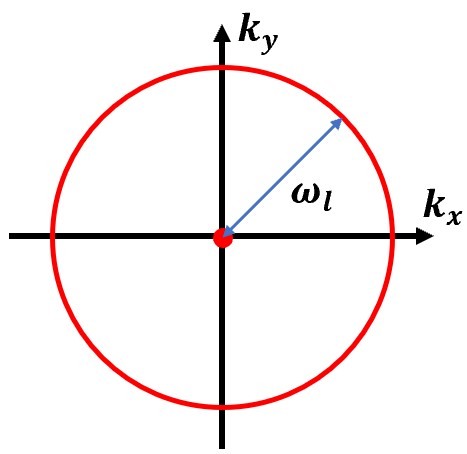
\includegraphics[width=\linewidth]{images/3D_SIM_OTF_no_angle_2D_plot_xy_k_l.jpg}
		\caption{}
		\label{fig:WF_OTF_xy}
	\end{subfigure}
	\begin{subfigure}[t]{0.4\textwidth}
		\centering
		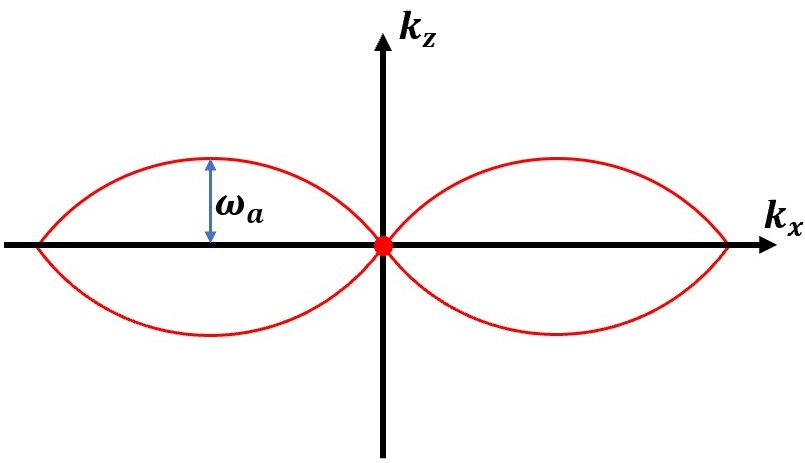
\includegraphics[width=\linewidth]{images/3D_SIM_OTF_no_angle_2D_plot_xz_k_a.jpg}
		\caption{}
		\label{fig:WF_OTF_xz}
	\end{subfigure}
	\begin{subfigure}[t]{0.27\textwidth}
		\centering
		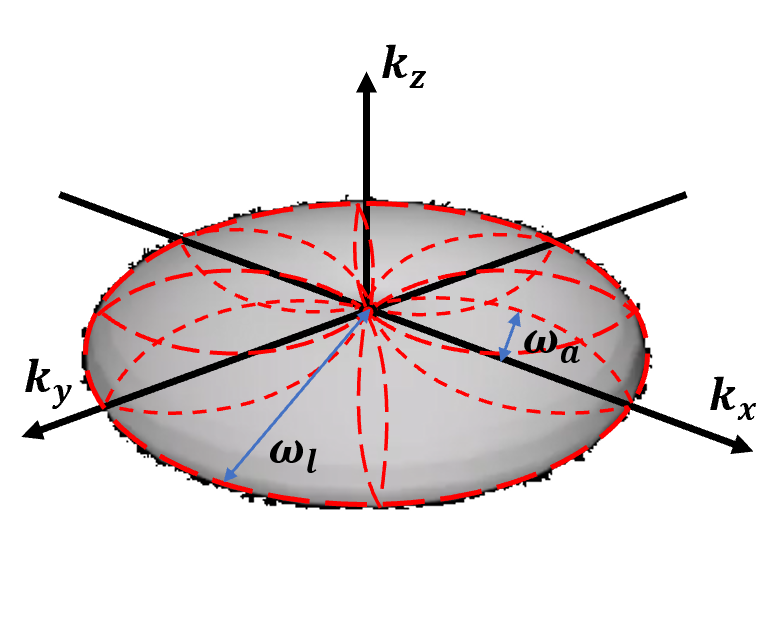
\includegraphics[width=\linewidth]{images/3D_SIM_OTF_no_angle_axis.png}
		\caption{}
		\label{fig:WF_OTF}
	\end{subfigure}
	\caption[Widefield observable region visualisation]{Widefield observable 
		region visualisation. \textbf{(a)} The projection of the observable 
		region onto the $k_{x}k_{y}$ plane. \textbf{(b)} The projection of 
		the observable region onto the $k_{x}k_{z}$ plane. \textbf{(c)} The 
		full observable region for a conventional widefield microscope in 
		reciprocal space.}
	\label{fig:widefield_OTF_visualisation}
\end{figure}

\section{Super-resolution Microscopy}
\label{sec:super_res}

For some time, the diffraction limit represented a kind of practical 
resolution asymptote - a point to be approached by never reached. Two
`gold standard' techniques for optical bioimaging emerged thanks to their
ease of implementation and how close they were able to get to the diffraction
limit; deconvolution\cite{agard1983three, wallace2001workingperson} and
confocal laser scanning microscopy\cite{sheppard1981theory,minsky1988memoir}. 
Nonetheless, the instant one defines a limit it is practically human nature 
to attempt to surpass it. Therefore, a number of `super-resolution' techniques
have emerged capable of surpassing even the ideal diffraction limit. These
can be broadly divided into two categories: near-field and far-field methods.
Near-field methods, whilst capable of achieving resolutions of $\sim 20 nm$,
are only suitable for surface structure imaging\cite{schermelleh2010guide}. 
Far-field techniques fall into 4 broad techniques: structured illumination
microscopy (SIM), stimulated emission depletion (STED) microscopy, 
single-molecule localisation microscopy (SMLM) and interferometric-based 
techniques. There are some implementations which combine several 
techniques. Each super-resolution technique has benefits and drawbacks which 
need to be considered when employing them including; the resolution 
(laterally and axially) required and the resolution achievable with each 
technique, acquisition speed, photodamage incurred, depth of imaging and 
multi-colour capability\cite{hell20152015,schermelleh2019super} Although it 
has a modest resolution improvement, SIM is the most widely accepted 
super-resolution technique for biology thanks to its multi-colour capability,
high temporal resolution and low photodamage impact\cite{leung2011review}.

\subsection{Structured Illumination Microscopy}
\label{subsec:SIM}

There are a number of microscopy techniques which fall under the structured
illumination microscopy umbrella: Re-scan\cite{de2013re}, 
Airyscan\cite{huff2015airyscan}, iSIM\cite{york2013instant,curd2015construction},
and SIMFlux\cite{cnossen2020localization} to name a few. Whilst all these can be 
considered `structured illumination' techniques since they do rely on spatially 
structured excitation light, for the duration of this thesis the term 
`structured illumination microscopy' or SIM refers to the form of 
interference-based microscopy pioneered by Mats 
Gustafsson\cite{gustafsson1999extended,gustafsson2000surpassing,gustafsson2008three}.
This implementation of SIM is best understood through the moir\'{e} effect.
Two patterns, such as those shown in Figure~\ref{fig:fringes_1} and 
\ref{fig:fringes_1}, which are multiplicatively superimposed on one another
will produce a beat pattern - moir\'{e} fringes - such as those shown in
Figure~\ref{fig:fringes_moire}. Using the convolution theorem, the Fourier
transform if this superposition is equivalent to the convolution of the 
Fourier transforms of the two original patterns\cite{mcgillem1991continuous},
as shown in Figures~\ref{fig:fringes_1_ft}-\ref{fig:fringes_moire_ft}. 

\begin{figure}[h]
	\centering
	\begin{subfigure}[t]{0.3\textwidth}
		\centering
		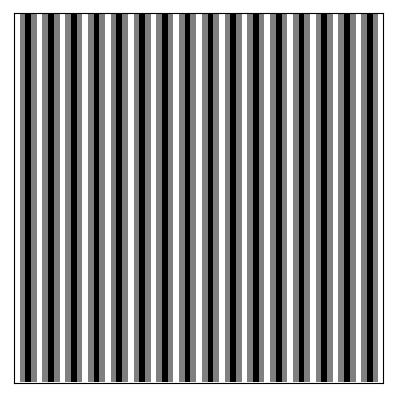
\includegraphics[width=\linewidth]{images/fringes_1_kx_16_ky_0.png}
		\caption{}
		\label{fig:fringes_1}
	\end{subfigure}
	\begin{subfigure}[t]{0.3\textwidth}
		\centering
		
\includegraphics[width=\linewidth]{images/fringes_2_kx_12_ky_12.png}
		\caption{}
		\label{fig:fringes_2}
	\end{subfigure}
	\begin{subfigure}[t]{0.3\textwidth}
		\centering
		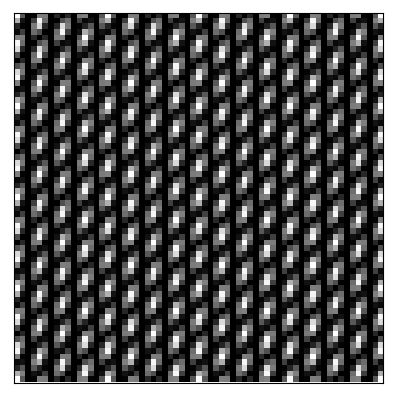
\includegraphics[width=\linewidth]{images/fringes_moire_kx_16_and_12_ky_0_and_12.png}
		\caption{}
		\label{fig:fringes_moire}
	\end{subfigure}
	
	\begin{subfigure}[t]{0.3\textwidth}
		\centering
		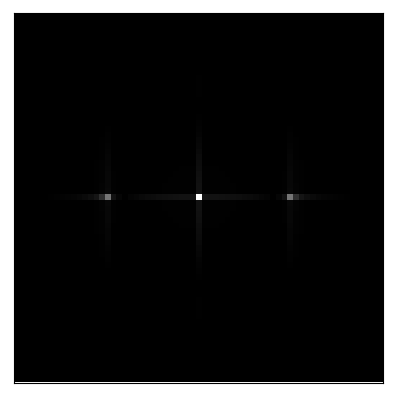
\includegraphics[width=\linewidth]{images/fringes_1_ft_kx_16_ky_0.png}
		\caption{}
		\label{fig:fringes_1_ft}
	\end{subfigure}
	\begin{subfigure}[t]{0.3\textwidth}
		\centering
		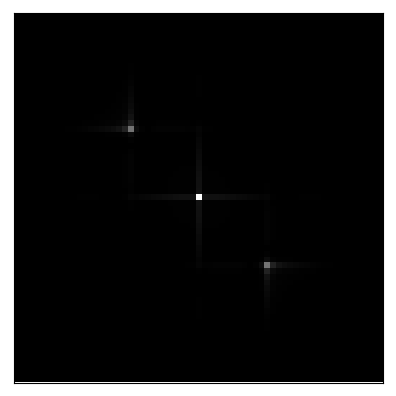
\includegraphics[width=\linewidth]{images/fringes_2_ft_kx_12_ky_12.png}
		\caption{}
		\label{fig:fringes_2_ft}
	\end{subfigure}
	\begin{subfigure}[t]{0.3\textwidth}
		\centering
		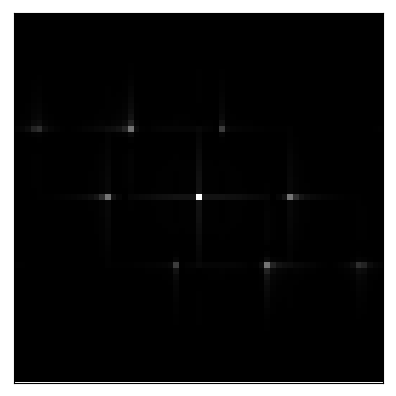
\includegraphics[width=\linewidth]{images/fringes_moire_ft_kx_16_and_12_ky_0_and_12.png}
		\caption{}
		\label{fig:fringes_moire_ft}
	\end{subfigure}
	\caption[Visualisation of moir\'{e} fringes]{Visualisation of moir\'{e} 
		fringes. \textbf{(a)}-\textbf{(b)} shows two spatially structured images. 
		\textbf{(c)} shows the resultant moir\'{e} fringes arising from the 
		interference of \textbf{(a)} and \textbf{(b)}. \textbf{(d)}-\textbf{(f)} 
		shows the respective Fourier transforms of \textbf{(a)}-\textbf{(c)}. 
		Note that \textbf{(f)} is a convolution of \textbf{(d)} and \textbf{(e)}}
	\label{fig:moire_visualisation}
\end{figure}

For SIM, one of the patterns is the underlying biological structure - or more 
specifically the spatial distribution of fluorophores - and the other is the 
spatially structured excitation illumination. The moir\'{e} fringes arising 
from the superposition of these two structures can be coarser than either of 
the original patterns, meaning that moir\'{e} fringes arising from the 
superposition of biological structures beyond the resolution limit of the 
microscope and a known illumination pattern can be observed. These moir\'{e} 
fringes contain information about these super-resolution structures and the
super-resolution information can be extracted from the moir\'{e} fringes, 
effectively extending the observable region of a microscope beyond the 
diffraction limit\cite{gustafsson2000surpassing}.

A single fluorescent image, $F(\textbf{r})$, is defined by:

\begin{equation}\label{eq:fluorescent_image}
\begin{split}
F(\textbf{r}) &= (E \circledast H)(\textbf{r})\\
F(\textbf{r}) &= [D(\textbf{r})I(\textbf{r})] \circledast H(\textbf{r}),\\
\end{split},
\end{equation}

Where $D(\textbf{r})$ is the sample fluorescence distribution, 
$I(\textbf{r})$ is the illumination pattern, $E(\textbf{r})$ is the resultant 
emission signal, $H(\textbf{r})$ is the system point spread function (PSF) 
and $\circledast$ represents the convolution operation. Applying the 
convolution theorem and a Fourier transform yield:

\begin{equation}\label{eq:SIM_fluorescent_image_fourier}
\begin{split}
\mathcal{F}\left[F(\textbf{r})\right] &= \mathcal{F}\left[\left[D(\textbf{r})I(\textbf{r})\right] \circledast H(\textbf{r})\right]\\
\tilde{F}(\textbf{k}) &= \left[\tilde{D}(\textbf{k})\circledast \tilde{I}(\textbf{k})\right] \tilde{H}(\textbf{k})\\
\tilde{F}(\textbf{k}) &= \left[\tilde{D}(\textbf{k})\circledast \tilde{I}(\textbf{k})\right] O(\textbf{k}),\\
\end{split},
\end{equation}

Where $\sim$ indicated the Fourier transform of the respective real-space
functions. $O(\textbf{k}) = \tilde{H}(\textbf{k})$ is the optical transfer
function (OTF) of the imaging system. The complex values of $O(\textbf{k})$
describe the attenuation of the spatial frequencies within the observable 
region described by Equation~\ref{eq:observable region}. For uniform 
illumination - i.e. widefield imaging - $\tilde{I}(\textbf{k}) = \delta(0)$ 
where $\delta$ is the Dirac delta function, and therefore only the spatial 
frequencies within the observable region contribute to the image formation as 
previously noted.  However, if $I(\textbf{r})$ is spatially structured then 
the convolution $\tilde{D}(\textbf{k})\circledast \tilde{I}(\textbf{k})$ is 
non-local and the  data within the observable region contains contributions 
from spatial frequencies which are normally outside the observable region.

For a general illumination pattern, extracting these super-resolution 
contributions from the diffraction limited contributions is non-trivial.
However, imposing some conditions on the illumination structure simplifies
this process\cite{gustafsson2008three}. Firstly, the illumination pattern 
should consist of the sum of a finite number, $m$, of components and these
components should be separable into axial and lateral components. The 
illumination pattern, $I(\textbf{r}_{xy},z)$, is therefore:

\begin{equation}\label{eq:illumination_components}
I(\textbf{r}_{xy},z) = \sum\limits_{m}{I_{m}(z)J_{m}(\textbf{r}_{xy})},
\end{equation}

where $\textbf{r}_{xy}$ the vector denoting the lateral coordinates, $(x,y)$.
Secondly, the lateral functions, $J_{m}(\textbf{r}_{xy})$, should be purely
harmonic functions meaning they contain only one spatial frequency. Note that 
the lateral functions, $J_{m}$, should not be confused with the first-order 
Bessel functions, $\mathcal{J}_{1}$ from before. Finally, the axial 
functions, $I_{m}(z)$, should either: 

\begin{enumerate}
	\item also be purely harmonic functions.
	\item in instances where 3D data is acquired as a series of 2D images with 
	different focus - as in microscopy - the illumination pattern is maintained 
	fixed relative to the focal plane of the microscope and not relative to the
	objecting being imaged.
\end{enumerate}

The first and third conditions allow Equation~\ref{eq:fluorescent_image} to be
written as:

\begin{equation}\label{eq:fluorescent_image_conditions}
\begin{split}
F(\textbf{r}) &= [D(\textbf{r})I(\textbf{r})] \circledast H(\textbf{r})\\
F(\textbf{r}) &= \sum\limits_{m}{\int H(\textbf{r}-\textbf{r}'))I_{m}(z - z')D(\textbf{r}')J_{m}(\textbf{r}'_{xy})}d\textbf{r}'\\
F(\textbf{r}) &= \sum\limits_{m}{\left[HI_{m}\circledast DJ_{m}\right](\textbf{r})}\\
\end{split},
\end{equation}

where $\textbf{r}'$ denotes the sample reference from, $\textbf{r}$ denotes
the data-set reference frame and $\textbf{r} - \textbf{r}'$ denotes the 
reference frame of the objective. Taking the Fourier transform of the 
$m$-th term, $F_{m}(\textbf{r})$, yields:

\begin{equation}\label{eq:fluorescent_image_mth_ft}
\tilde{F}_{m}(\textbf{k}) = \tilde{O}_{m}\left[\tilde{D}(\textbf{k}) \circledast \tilde{J}_{m}(\textbf{k}_{xy})\right],
\end{equation}

where $\tilde{O}_{m} = O \circledast \tilde{I}_{m} = \mathcal{F}[HI_{m}]$.
Here the second condition of the lateral functions being purely harmonic allows
$J_{m}(\textbf{r}_{xy})$ to be written as:

\begin{equation}\label{eq:lateral_illumination}
J_{m}(\textbf{r}_{xy}) = e^{i\left(2\pi\textbf{p}_m\cdot\textbf{r}_{xy} + \phi_{m}\right)},
\end{equation}

\begin{equation}\label{eq:lateral_illumination_ft}
\Rightarrow \tilde{J}_{m}(\textbf{k}_{xy}) = \delta\left(\textbf{k}_{xy} - \textbf{p}_m\right)e^{i\phi_{m}},
\end{equation}

Substituting Equation~\ref{eq:lateral_illumination_ft} into 
Equation~\ref{eq:fluorescent_image_mth_ft} and summing over all $m$ components,
the observed data can be written as:

\begin{equation}\label{eq:single_SIM_image}
\tilde{F}(\textbf{k}) = \sum\limits_{m}{\tilde{O}_{m}(\textbf{k})e^{i\phi_{m}}\tilde{D}\left(\textbf{k} - \textbf{p}_m\right)}.
\end{equation}

Therefore, each image is a sum of a finite number, $N$, copies of the object 
information, $\tilde{D}$, each shifted laterally in reciprocal space by 
$\textbf{p}_{m}$, filtered by the OTF, $O$, and phase shifted by $\phi_{m}$.
Acquiring $N$ images with different values of $\phi_{m}$ gives a system of 
linear equations with as many equations as unknowns. The frequency components
can therefore be separated by applying an $N\times N$ separation matrix. The 
values of $\phi_{m}$ are generally chosen to be evenly spaced between 
$[0,2\pi]$ radians to ensure a well-conditioned separation 
matrix\cite{gustafsson2008three}.

Considering the practical implications further simplifies the situation. 
Firstly, the intensity distribution of light is a real-valued function and
therefore the exponentials in Equation~\ref{eq:lateral_illumination_ft} must
occur in pairs with $\pm\textbf{p}_{m}$. Since the Fourier transform of a 
real-valued function has the symmetry property $\tilde{a}(-\textbf{k}) = 
\bar{\tilde{a}}(\textbf{k})$ only one component need be calculated and the
other can be determined by symmetry. Secondly, if the $\textbf{p}_{m}$ are
chosen such that they are all either the fundamental frequency or higher 
harmonics of the same frequency then $\textbf{p}_{m} = m\textbf{p}$ where
$\textbf{p}$ is the fundamental frequency. Furthermore, if the phases are 
chosen such that $\phi_{m} = m\phi$. Taking these effects into account, 
Equation~\ref{eq:single_SIM_image} becomes:

\begin{equation}\label{eq:single_SIM_image_simple}
\tilde{F}(\textbf{k}) = \sum\limits_{m}{\tilde{O}_{m}(\textbf{k})e^{im\phi}\tilde{D}\left(\textbf{k} - m\textbf{p}\right)}.
\end{equation}

Since $O_{m}$ and $\textbf{p}_{m}$ are known, the information components
can be separated and moved by $\textbf{p}_{m}$ back to their correct 
position in reciprocal space, combined to a single extended resolution
spatial frequency dataset, and finally Fourier transformed back into a 
single super-resolution image.  From Equation~\ref{eq:single_SIM_image} 
it is clear that this image is equivalent to an image taken with an 
observable region equal to the convolution of the original system OTF, 
$O$, and the illumination structure Fourier transform, $\tilde{I}$. 

Consider an illumination pattern formed by the interference of two beams 
of light such that $I(\textbf{r}) \propto 1 + \cos(\textbf{r}\cdot
\textbf{p} + \phi)$. Figure~\ref{fig:amplitude_wave_vectors_2D} shows 
the amplitude wave vectors for these beams, both with the same length 
$\frac{1}{\lambda_{ex}}$ where $\lambda_{ex}$ is the wavelength of the 
excitation illumination light. The angle between the two beams determines 
the position of $\textbf{p}$. If $\textbf{p}$ is chosen to be close to 
$k_{l}$ then the spatial frequency components are close to the bounds 
of the observable region, as shown in 
Figure~\ref{fig:2D_SIM_OTF_beam_pos_w_vectors}. The convolution of this 
illumination pattern with the system OTF is shown in 
Figure~\ref{fig:2D_SIM_OTF_1_angle}. The projection of this extended 
observable region on the $k_{x}k_{z}$ plane is shown in 
Figure~\ref{fig:2D_SIM_OTF_1_angle_plot_xz}. The observable region
is laterally extended by a factor, $\alpha_{l}$, given by:

\begin{equation}\label{eq:lateral_res_extension_factor}
\alpha_{l} = \frac{\left(\frac{1}{\lambda_{ex}} + \frac{1}{\lambda_{em}}\right)}{\frac{1}{\lambda_{em}}} = 1 + \frac{\lambda_{em}}{\lambda_{ex}},
\end{equation}

where $\lambda_{ex}$ and $\lambda_{em}$ are the excitation and emission
wavelengths respectively.  However, this extension factor only applied in 
the direction $\overrightarrow{\textbf{p}}$. To achieve isotropic 
resolution enhancement, a number of pattern directions are required. 
Rotating the illumination pattern through the three stripe angles shown 
in Figure~\ref{fig:3D_SIM_OTF_stripe_angles} yields the extended 
observable region in Figure~\ref{fig:2D_SIM_OTF_all_2D_angles}, the 
projection of which in the $k_{x}k_{y}$ plane is shown in
Figure~\ref{fig:3D_SIM_OTF_xy_expansion_w_double_rad_filled}. 

\begin{figure*}
	\centering
	\begin{subfigure}[t]{0.25\textwidth}
		\centering
		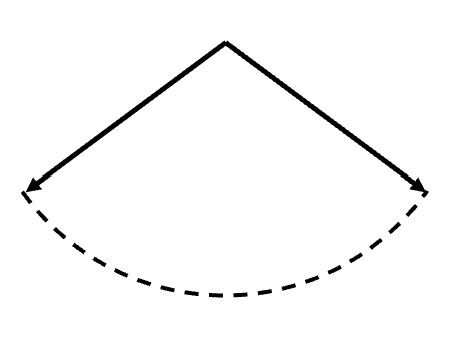
\includegraphics[width=\linewidth]{images/amplitude_wave_vectors_2D.jpg}
		\caption{}
		\label{fig:amplitude_wave_vectors_2D}
	\end{subfigure}
	\begin{subfigure}[t]{0.265\textwidth}
		\centering
		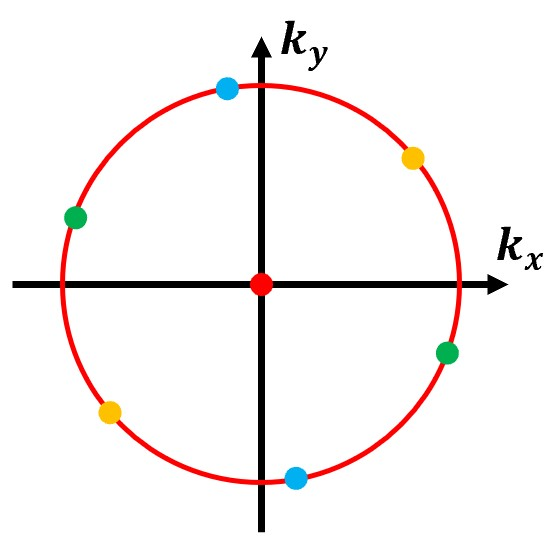
\includegraphics[width=\linewidth]{images/3D_SIM_OTF_stripe_angles.jpg}
		\caption{}
		\label{fig:3D_SIM_OTF_stripe_angles}
	\end{subfigure}
	\begin{subfigure}[t]{0.45\textwidth}
		\centering
		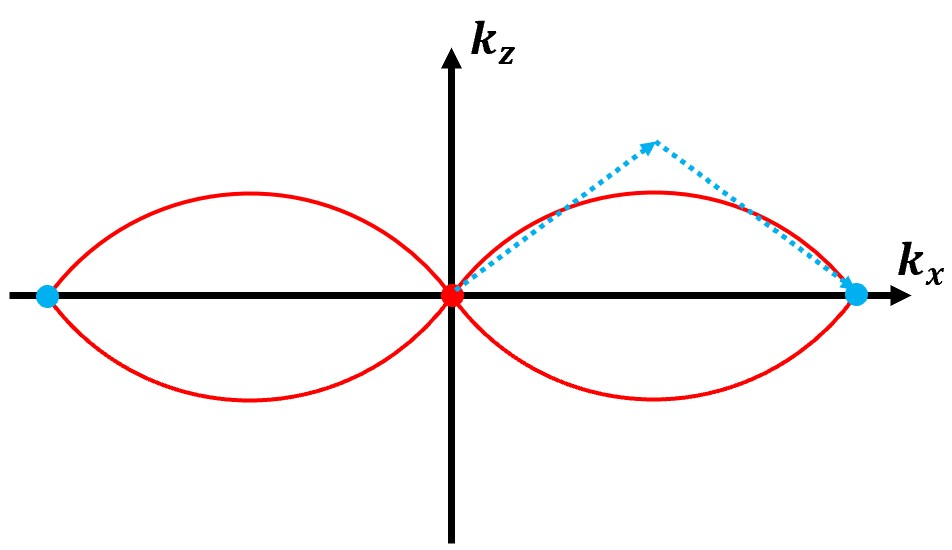
\includegraphics[width=\linewidth]{images/2D_SIM_OTF_beam_pos_w_vectors.jpg}
		\caption{}
		\label{fig:2D_SIM_OTF_beam_pos_w_vectors}
	\end{subfigure}
	
	\begin{subfigure}[t]{0.35\textwidth}
		\centering
		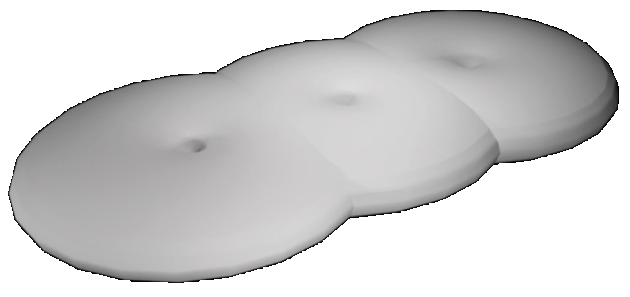
\includegraphics[width=\linewidth]{images/3D_SIM_OTF_1_angle.png}
		\caption{}
		\label{fig:2D_SIM_OTF_1_angle}
	\end{subfigure}
	\begin{subfigure}[t]{0.6\textwidth}
		\centering
		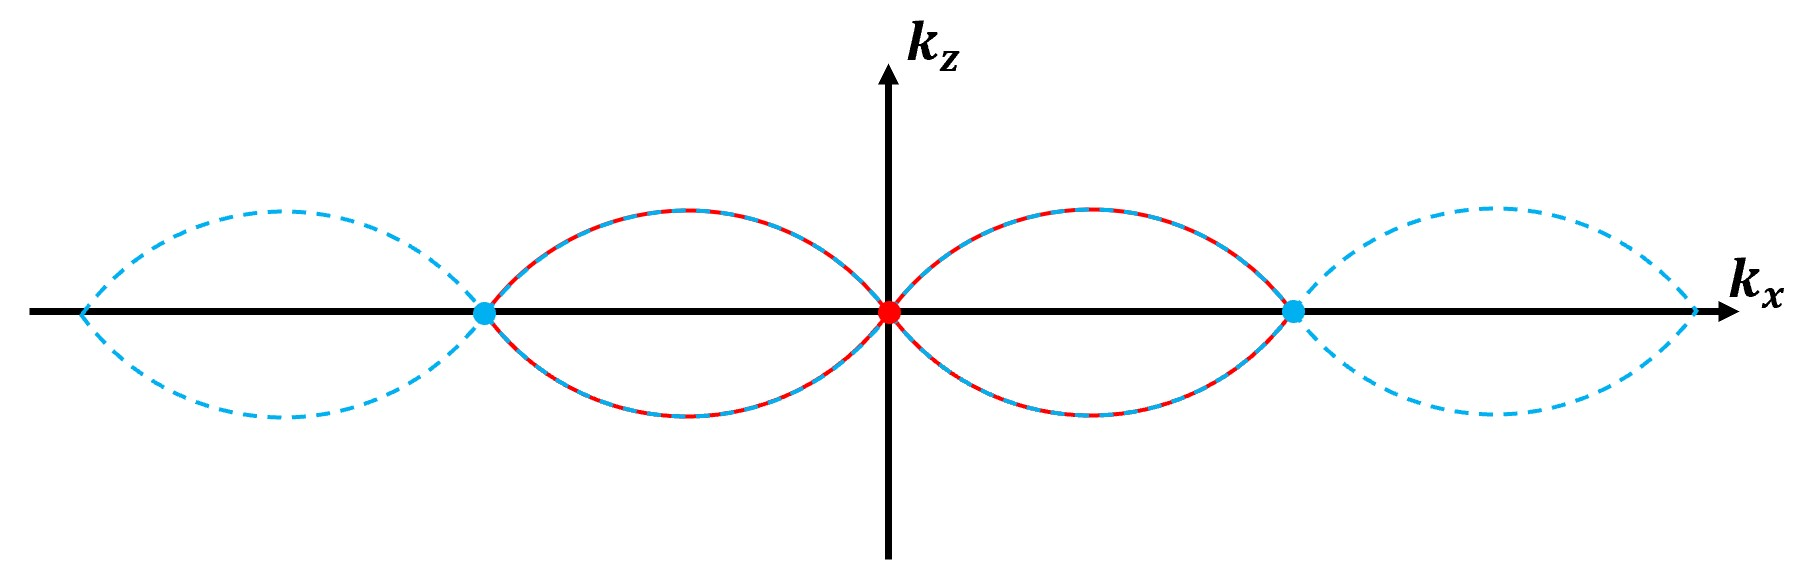
\includegraphics[width=\linewidth]{images/2D_SIM_OTF_1_angle_plot_xz.jpg}
		\caption{}
		\label{fig:2D_SIM_OTF_1_angle_plot_xz}
	\end{subfigure}
	
	\begin{subfigure}[t]{0.4\textwidth}
		\centering
		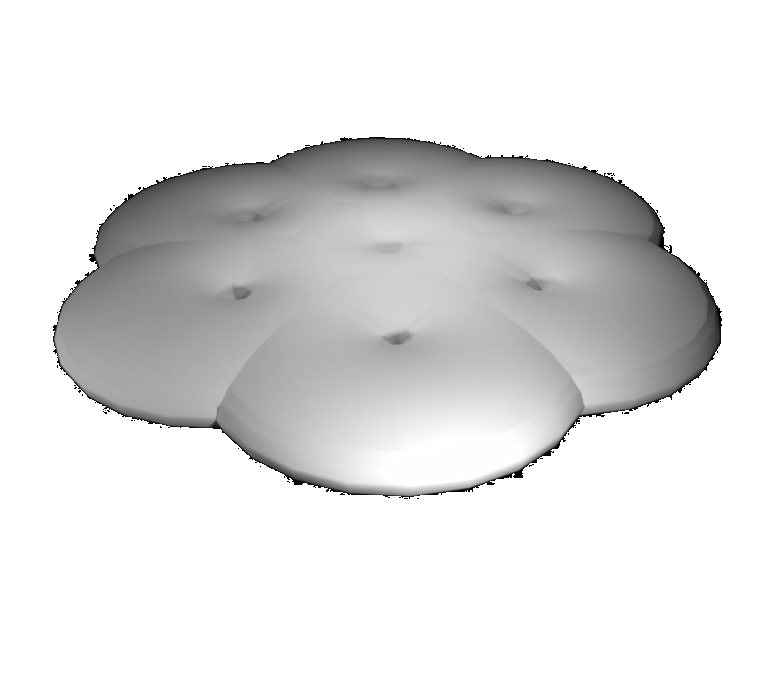
\includegraphics[width=\linewidth]{images/2D_SIM_OTF_all_2D_angles.png}
		\caption{}
		\label{fig:2D_SIM_OTF_all_2D_angles}
	\end{subfigure}
	\begin{subfigure}[t]{0.5\textwidth}
		\centering
		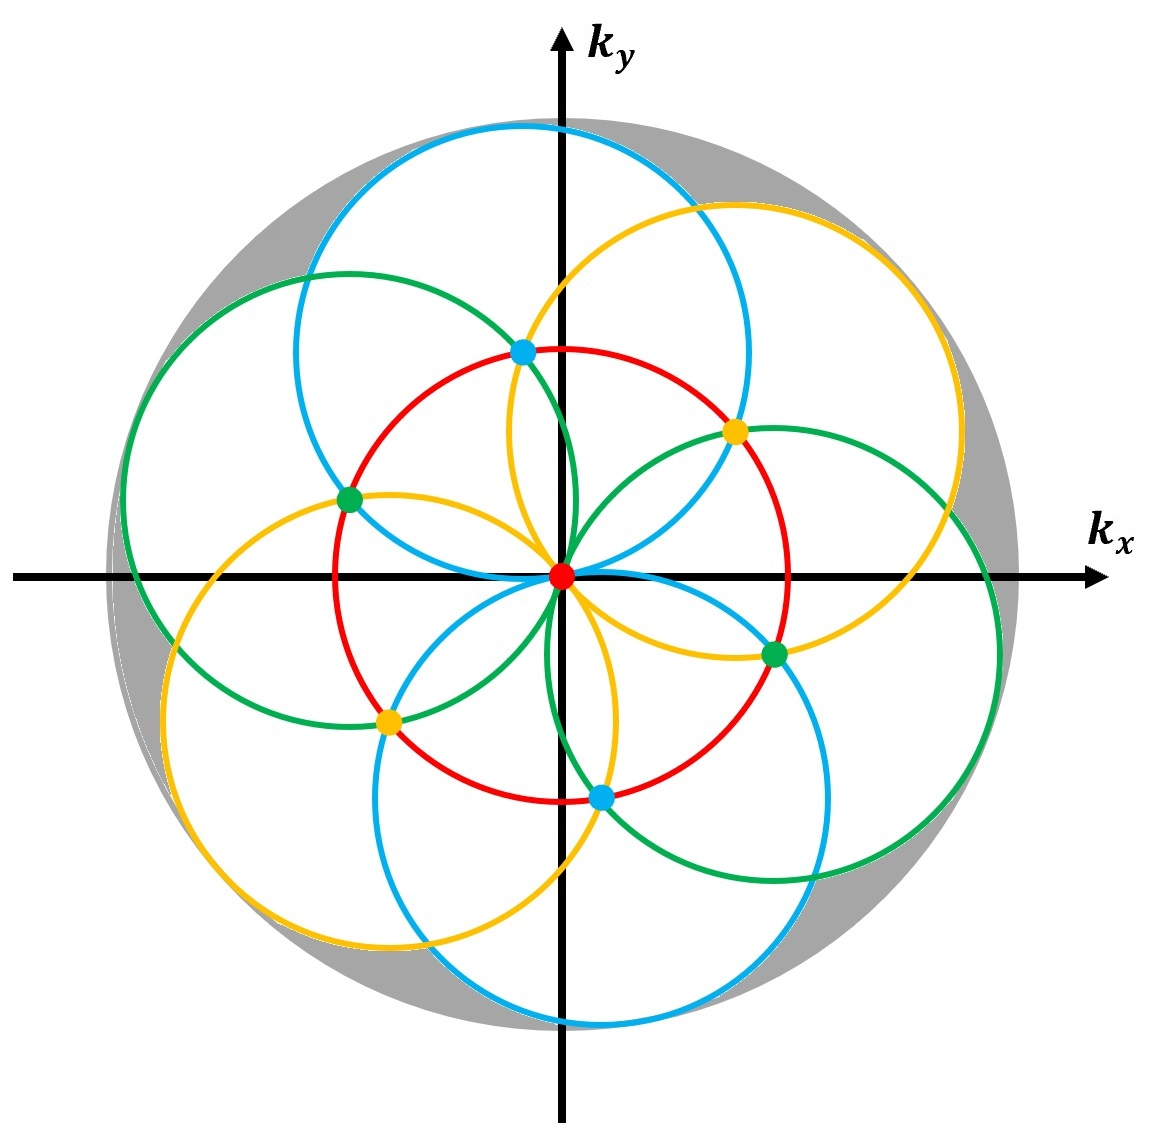
\includegraphics[width=\linewidth]{images/3D_SIM_OTF_xy_expansion_w_double_rad_filled.jpg}
		\caption{}
		\label{fig:3D_SIM_OTF_xy_expansion_w_double_rad_filled}
	\end{subfigure}
	\caption[Resolution enhancement with 2D SIM imaging]{Resolution enhancement 
		with 2D SIM imaging. \textbf{(a)} The amplitude wave vectors 
		corresponding to the 2 illumination beams. Both vectors have the 
		same magnitude, $\frac{1}{\lambda}$ \textbf{(b)} The projection of the 
		observable region onto the $k_{x}k_{y}$ plane with the stripe angles 
		shown \textbf{(c)} The projection of the observable region onto the 
		$k_{x}k_{z}$ plane with the spatial frequency component locations for
		two-beam interference pattern shown. \textbf{(d)} The full observable region 
		extension for one angle in reciprocal space. \textbf{(e)} The projection 
		of the extended observable region in \textbf{(d)} onto the $k_{x}k_{z}$ 
		plane. \textbf{(f)} The full observable region extension for all three angles in 
		reciprocal space. \textbf{(g)} The projection of the extended observable 
		region in \textbf{(f)} onto the $k_{x}k_{y}$ plane. The shaded grey area
		shows the reciprocal components missing for an isotropic observable region
		extension factor $\alpha_{l}$.}
	\label{fig:2D_SIM_visualisation}
\end{figure*}

Figure~\ref{fig:3D_SIM_OTF_xy_expansion_w_double_rad_filled} shows
that whilst there is an expansion of the observable region in all
directions in the $k_{x}k_{y}$ plane, it is not a lateral isotropic 
extension by $\alpha_{l}$. Nonetheless, it is still sufficient to yield 
a doubling of the lateral resolution\cite{gustafsson2000surpassing}.
This choice of illumination structure still suffers from the missing
cone problem noted in Section~\ref{subsec:resolution}, meaning there
is no improvement in axial resolution.

Now consider an illumination pattern formed by three light beams with
wave vectors, $\textbf{k}_{j}$, such as those shown in 
Figure~\ref{fig:amplitude_wave_vectors}. The 3D interference pattern, 
$I(\textbf{r})$ generated by the superposition of these waves:

\begin{equation}\label{eq:3_beam_interference}
\begin{split}
I(\textbf{r}) \propto \left|\sum\limits_{j}{\textbf{E}_{j}e^{i\textbf{k}_j\cdot\textbf{r}}}\right|^{2} &= \left(\sum\limits_{j}{\textbf{E}^{*}_{j}e^{-i\textbf{k}_{j}\cdot\textbf{r}}}\right)
\left(\sum\limits_{q}{\textbf{E}_{q}e^{i\textbf{k}_{q}\cdot\textbf{r}}}\right)\\
&= \sum\limits_{j,q}{\textbf{E}^{*}_{j}\cdot\textbf{E}_{q}e^{-i\left(\textbf{k}_{q}-\textbf{k}_{j}\right)\cdot\textbf{r}}},
\end{split}
\end{equation}

therefore has 7 Fourier components located at each of the pairwise
difference vectors, $\left(\textbf{k}_{q}-\textbf{k}_{j}\right)$, 
between the any two of the beam wave vectors. The location of these 
Fourier components is shown in 
Figure~\ref{fig:3D_SIM_OTF_beam_pos_w_vectors}. The convolution of 
this interference pattern, rotated through the stripe angles shown
in Figure~\ref{fig:3D_SIM_OTF_stripe_angles}, yields the extended
observable region shown in Figure~\ref{fig:3D_SIM_OTF_all_angles}.
The projection of the extended observable region for one of these 
stripe angles onto the $k_{x}k{z}$ plane is shown in 
Figure~\ref{fig:3D_SIM_OTF_1_angle_2D_plot}. The addition of the
Fourier component off the $k_{x}$ axis has the effect of filling 
in the missing cone. From this plot it may appear that there are
now two missing cones above and below the off-$k_{x}$-axis components.
However, as Figure~\ref{fig:3D_SIM_OTF_1_angle_2D_plot} shows, 
since these Fourier components are closer together than the
on-axis components, much of these missing cones is filled out by 
the rotation of the interference pattern through several stripe
angles. Taken together, the extension of the observable region 
yields a super-resolution image with an isotropic resolution 
doubling compared to a diffraction limited 
system\cite{gustafsson2008three}.

\begin{figure*}
	\centering
	\begin{subfigure}[t]{0.35\textwidth}
		\centering
		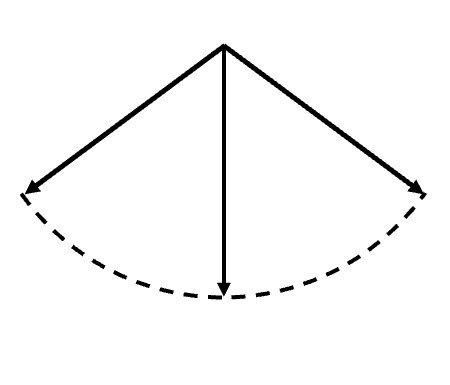
\includegraphics[width=\linewidth]{images/amplitude_wave_vectors.jpg}
		\caption{}
		\label{fig:amplitude_wave_vectors}
	\end{subfigure}
	\begin{subfigure}[t]{0.6\textwidth}
		\centering
		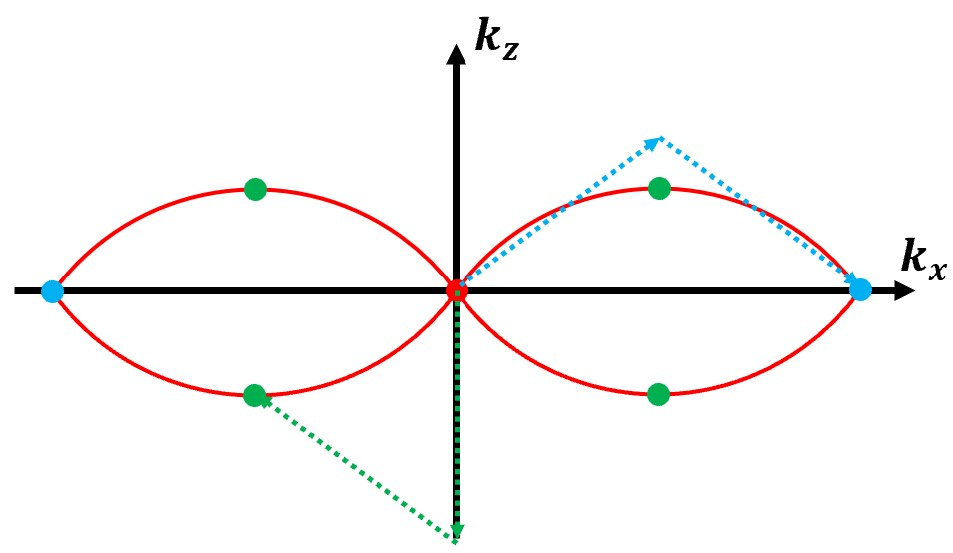
\includegraphics[width=\linewidth]{images/3D_SIM_OTF_beam_pos_w_vectors.jpg}
		\caption{}
		\label{fig:3D_SIM_OTF_beam_pos_w_vectors}
	\end{subfigure}
	
	\begin{subfigure}[t]{0.35\textwidth}
		\centering
		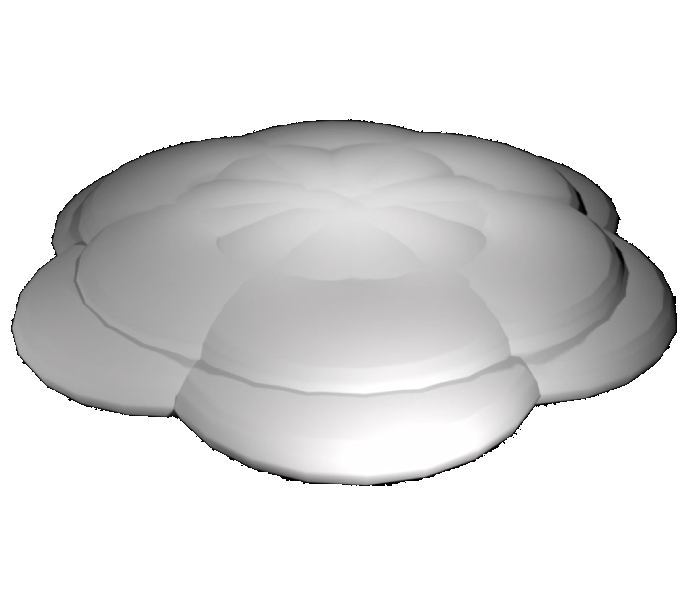
\includegraphics[width=\linewidth]{images/3D_SIM_OTF_all_angles.png}
		\caption{}
		\label{fig:3D_SIM_OTF_all_angles}
	\end{subfigure}
	\begin{subfigure}[t]{0.625\textwidth}
		\centering
		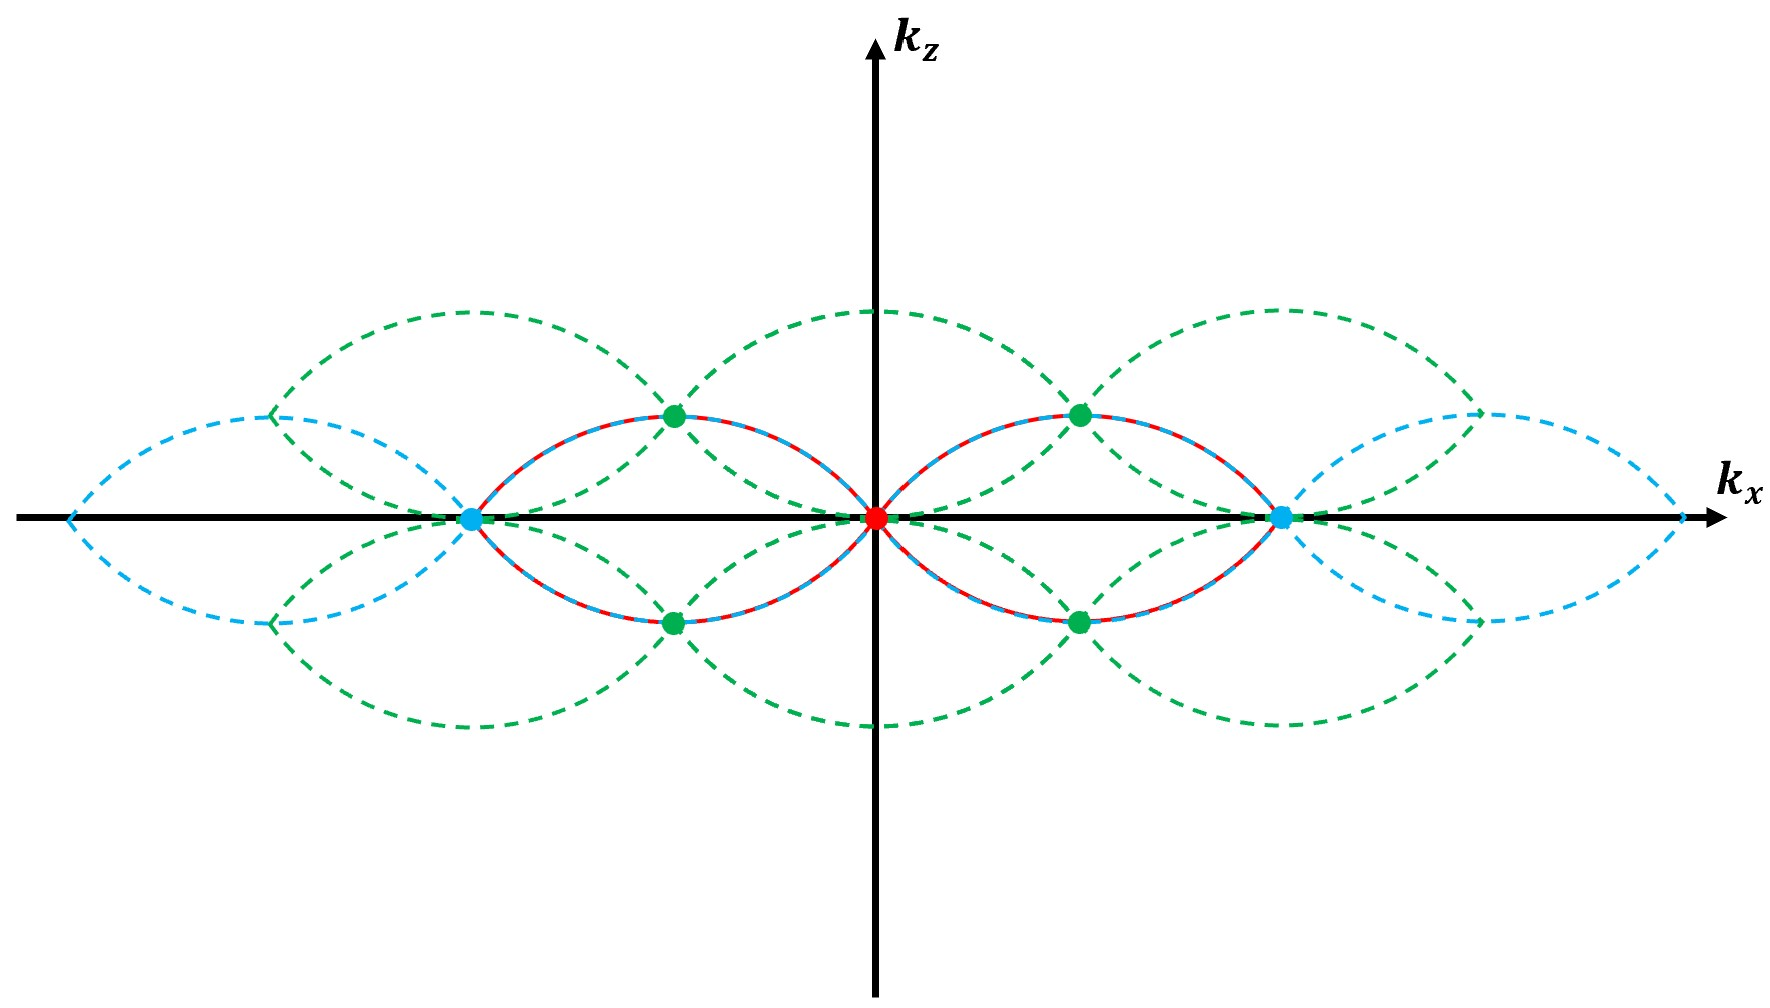
\includegraphics[width=\linewidth]{images/3D_SIM_OTF_1_angle_2D_plot.jpg}
		\caption{}
		\label{fig:3D_SIM_OTF_1_angle_2D_plot}
	\end{subfigure}	
	\caption[Resolution enhancement with 3D SIM imaging]{Resolution enhancement 
		with 3D SIM imaging. \textbf{(a)} The amplitude wave vectors 
		corresponding to the 3 illumination beams. All vectors have the 
		same magnitude, $\frac{1}{\lambda}$ \textbf{(b)} The projection of the 
		observable region onto the $k_{x}k_{z}$ plane with the spatial frequency 
		component locations for three-beam interference patterns shown. 
		\textbf{(c)} The full observable region extension for all three angles in 
		reciprocal space. \textbf{(d)} The projection of the extended observable 
		region for one stripe angle onto the $k_{x}k_{z}$ plane.}
	\label{fig:3D_SIM_visualisation}
\end{figure*}

As previously mentioned, SIM is the most widely accepted 
super-resolution technique for biology for a number of reasons. The 
number of images required in order to reconstruct a super-resolution 
SIM image, are determined by the number of lateral Fourier components 
in the illumination pattern - 3 for 2D SIM and 5 for 3D SIM - and the
number of stripe angles used to rotate the illumination pattern through
- typically 3. Therefore, only 9 or 15 images are required to 
reconstruct a 2D or 3D super-resolution SIM image respectively. This
has a number of benefits. Firstly, the temporal resolution is 
considerably higher for SIM than for point-scanning super-resolution
techniques such as STED or SMLM techniques which require a great deal more 
images per reconstruction\cite{schermelleh2019super,leung2011review}.
Secondly, each of these images is fundamentally still a widefield-style
image and therefore has a lower light-dosage than per image than STED 
or SMLM techniques. The lower light-dosage per image combined with fewer
total images required per reconstruction contributes to a low 
photodamage impact. Finally, SIM is easily expandable to multi-colour 
imaging, even using the same optical 
setup\cite{wu2018faster,allen2014structured}. Overall, SIM is a 
super-resolution technique well suited to biological imaging, 
particularly imaging dynamic biological processes.

\section{Optical Aberrations}
\label{sec:aberrations}

One factor preventing microscopes from achieving the ideal diffraction
limited resolution is the presence of optical 
aberrations\cite{goodman2005introduction,wyant1992basic,wolf1951diffraction}.
These aberrations describe the deviation of the light wavefront
from the ideal Gaussian surface. They have numerous sources, but the most
common are those arising from system imperfections - i.e. manufacturing errors
in components, placement of lenses off the optical axis, etc - and those
arising refractive index variances across the 
wavefront\cite{kubby2013adaptive,booth2007adaptive}. In biological samples, 
these variances arise from sample heterogeneities since different biological
structures possess varied refractive 
indices\cite{bashkatov2011optical, jacques2013optical, kim2010measurement, sandell2011review}.
These refractive index variances introduce path differences between 
different section of the light wavefront. A generalised pupil function 
(GPF) defined as\cite{antonello2014optimisation}:

\begin{equation}\label{eq:GPF}
P\left(\textbf{r}_{xy}\right) = A\left(\textbf{r}_{xy}\right)e^{i\Phi\left(\textbf{r}_{xy}\right)},
\end{equation}

is a complex-valued function. Defining the GPF on the normalised system 
pupil and assuming the pupil is circular simplifies the following analysis
and is generally more intuitive. In such a system, the GPF has the form:

\begin{equation}\label{eq:GPF_polar}
P\left(\rho,\theta\right) = A\left(\rho,\theta\right)e^{i\Phi\left(\rho,\theta\right)}.
\end{equation}

The real-valued function $A\left(p,\theta\right)$ accounts for amplitude
aberrations and the real-valued function $\Phi\left(p,\theta\right)$ 
accounts for the phase aberrations. Revisiting the simplified optical
system in Figure~\ref{fig:simplified_microscope_layout}, assuming a point
source a $\textbf{O}$ and that the exit pupil of the system is the unit 
disk, the field intensity at the $x'y'$ plane is proportional 
to\cite{goodman2005introduction,born2013principles}:

\begin{equation}\label{eq:image_field_insentity_GPF}
\mathcal{I}(v,\phi) = \frac{1}{\pi}\left|\int^{1}_{0}\int^{2\pi}_{0}P\left(\rho,\theta\right)e^{iv\rho\cos(\theta-\phi)}\rho d\rho d\theta\right|^{2}.
\end{equation}

For an aberration free system, $A\left(\rho,\theta\right) = 1$ and 
$\Phi\left(\rho,\theta\right) = 0$ which makes the integral in 
Equation~\ref{eq:image_field_insentity_GPF} analytically computable. From 
this it is possible to recover $\mathcal{I}(v,\phi) = \mathcal{I}_{w}(v)$
from Equation~\ref{eq:image_field_insentity}.

\subsection{Zernike Polynomials}
\label{subsec:zernike}

Whilst the phase distortions can be treated in their native form, it is 
useful for a number of reasons to represent them as an expansion in
orthogonal functions, and Zernike polynomials are typically chosen for 
this expasion\cite{zernike1934diffraction,noll1976zernike,mahajan1994zernike}.
Zernike modes are not suitable to represent phase distortions arising 
from all sources, such as air turbulence or fabrication errors in the 
single-point diamond turning process\cite{wyant1992basic}. However, the 
sources of phase distortions for which a Zernike representation is not
appropriate do not generally arise. Additionally, the Zernike modes have 
a number of useful mathematical properties, and low order Zernike modes 
correspond to well-known optical aberrations e.g. defocus, astigmatism, 
coma, spherical 
aberration\cite{born2013principles,booth2007adaptive,zernike1934diffraction}.
Using the Zernike polynomials, the phase distortions, $\Phi\left(\rho,\theta\right)$
can be written as:

\begin{equation}\label{eq:phase_zernike_expansion}
\Phi\left(\rho,\theta\right) = \sum\limits_{n,m}\alpha^{m}_{n}\mathcal{Z}^{m}_{n}\left(\rho,\theta\right),
\end{equation}

where indices $n \in \mathbb{N}_{0}$ and $m \in \mathbb{Z}$ denote the radial order 
and azimuthal frequency respectively of the Zernike polynomial, 
$\mathcal{Z}^{m}_{n}$, and are such that $n - \left|m\right| \ge 0$ and even. The
coefficients of each Zernike polynomial are represented by $\alpha^{m}_{n} \in 
\mathbb{R}$. Each Zernike polynomial is the product of a radial polynomial,
$R^{m}_{n}(\rho)$, and an azimuthal polynomial, $\Theta^{m}_{n}(\theta)$:

\begin{equation}\label{eq:zernike_polynomial}
\mathcal{Z}^{m}_{n}\left(\rho,\theta\right) = c^{m}_{n}R^{m}_{n}(\rho)\Theta^{m}_{n}(\theta),
\end{equation}

where $c^{m}_{n}$, $R^{m}_{n}(\rho)$, and $\Theta^{m}_{n}(\theta)$ have the following definitions:

\begin{equation}\label{eq:zernike_polynomial_c}
c^{m}_{n} = 
\begin{cases}
\sqrt{n + 1} & m = 0\\
\sqrt{2(n + 1)} & m \ne 0\\
\end{cases},
\end{equation}

\begin{equation}\label{eq:zernike_polynomial_R}
R^{m}_{n}(\rho) = \sum_{s=0}^{\frac{n-m}{2}}{\frac{(-1)^{s}(n-s)!}{s!\left(\frac{n+m}{2}-s\right)!\left(\frac{n-m}{2}-s\right)!}\rho^{n-2s}},
\end{equation}

\begin{equation}\label{eq:zernike_polynomial_Theta}
\Theta^{m}_{n}(\theta) =
\begin{cases}
\cos(m\theta) & m \ge 0\\
-\sin(m\theta) & m < 0\\
\end{cases}.
\end{equation}

This formulation of Zernike modes is normalised and ordered according
to the Noll indexing convention, although other modal bases and ordering 
conventions do exist\cite{noll1976zernike,thibos2002standards,
	loomis1978computer,soloviev2017optimal,burton1984effects}. 

It is useful to be able to compare phase distortions to one another to
measure their severity. In order to do so, scalar indicators are required.
Typically, the root mean squared (rms) and variance of $\Phi\left(\rho,\theta\right)$
are used:

\begin{align}\label{eq:scalar_indicators}
rms(\Phi) = \left(E_{2}\left[\Phi\right]\right)^{\frac{1}{2}} && 
var(\Phi) = E_{2}\left[\Phi\right] - \left(E_{1}\left[\Phi\right]\right)^{2},
\end{align}

where $E_{k}\left[\Phi\right]$ are the 
functionals\cite{antonello2014optimisation,mahajan1994zernike}:

\begin{equation}\label{eq:E_functionals}
E_{k}\left[\Phi\right] = \frac{1}{\pi} \int_{0}^{1}\int_{0}^{2\pi} \Phi\left(\rho,\theta\right)^{k}\rho d\rho d\theta.
\end{equation}

Using the normalisation factors, $c_{n}^{m}$, and the orthogonality
properties of the Zernike modes, it is apparent that $E_{1}\left[\Phi\right] 
= \alpha_{0}^{0}$ and $E_{2}\left[\Phi\right] = 
\sum\limits_{n,m}{\left({\alpha_{n}^{m}}\right)^{2}}$. Substituting 
these values back into Equations~\ref{eq:scalar_indicators} yields:

\begin{align}\label{eq:scalar_indicators_new}
rms(\Phi) = \left(\sum\limits_{n,m}{\left({\alpha_{n}^{m}}\right)^{2}}\right)^{\frac{1}{2}} && 
var(\Phi) = \sum\limits_{n\ne 0,m\ne 0}{\left({\alpha_{n}^{m}}\right)^{2}},
\end{align}

Since $\mathcal{Z}_{n}^{m}$ - i.e. piston - does not affect image 
formation, often its corresponding amplitude $\alpha_{0}^{0}$ is
simply not included. In this case, $rms(\Phi) = \sqrt{var(\Phi)}$

\subsection{Aberrations and Resolution}
\label{subsec:aberrations_and_resolution}

Not all Zernike modes affect the resolution of the system. 
Figures~\ref{fig:Airy_ring_2D_2_object_seperation_aberration_comparison_Noll_1}-
\ref{fig:Airy_ring_2D_2_object_seperation_aberration_comparison_Noll_3}
show the effect of the first 3 Zernike modes, $\mathcal{Z}_{0}^{0}$, 
$\mathcal{Z}_{1}^{-1}$, and $\mathcal{Z}_{1}^{1}$ - i.e. piston, tip and 
tilt - on two point objects separated by the diffraction limit determined
by the Rayleigh criterion, $r_{l}$. Clearly piston has no effect on the 
image intensity or resolving power. Additionally, assuming an incoherent, 
shift invariant imaging system, the only effect of the tip and tilt 
aberrations is a lateral shift in the $x$ and $y$ axis respectively. The
overall image intensity and resolving power remains unaffected. For this 
reason piston (and often tip and tilt) are considered ``non-optical'' 
aberrations. 
Figure~\ref{fig:Airy_ring_2D_2_object_seperation_aberration_comparison_rms_1}
shows the same two point objects aberrated with phase deformations of 
$rms(\Phi) = 1$. The image intensity is severely degraded and the resolving
power is significantly less than the diffraction limited case. Evidently, 
the presence of phase distortions is a limiting factor to imaging systems 
from achieving the ideal diffraction limited 
resolution\cite{antonello2014optimisation,booth2014adaptive}.

\begin{figure*}
	\centering
	\begin{subfigure}{0.49\textwidth}
		\centering
		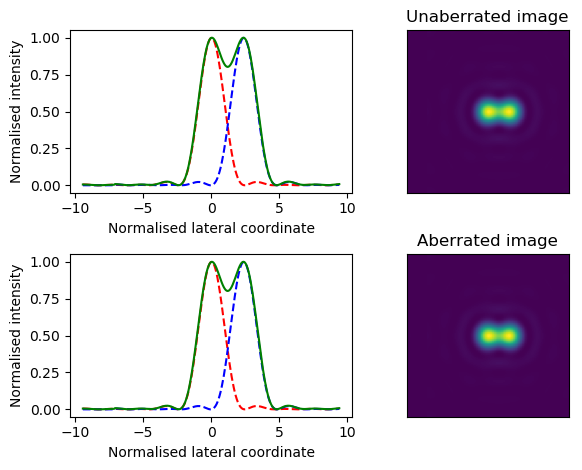
\includegraphics[width=\linewidth]{images/Airy_ring_2D_2_object_seperation_aberration_comparison_Noll_1.png}
		\caption{$rms(\Phi) = 1, \alpha_{0}^{0} = 1$}
		\label{fig:Airy_ring_2D_2_object_seperation_aberration_comparison_Noll_1}
	\end{subfigure}
	\begin{subfigure}{0.49\textwidth}
		\centering
		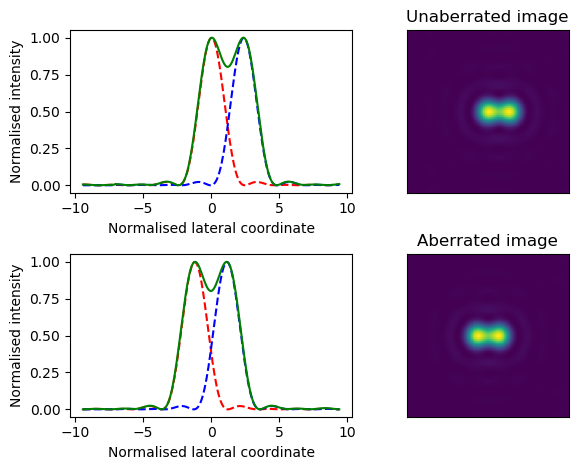
\includegraphics[width=\linewidth]{images/Airy_ring_2D_2_object_seperation_aberration_comparison_Noll_2.png}
		\caption{$rms(\Phi) = 1, \alpha_{1}^{-1} = 1$}
		\label{fig:Airy_ring_2D_2_object_seperation_aberration_comparison_Noll_2}
	\end{subfigure}
	\begin{subfigure}{0.49\textwidth}
		\centering
		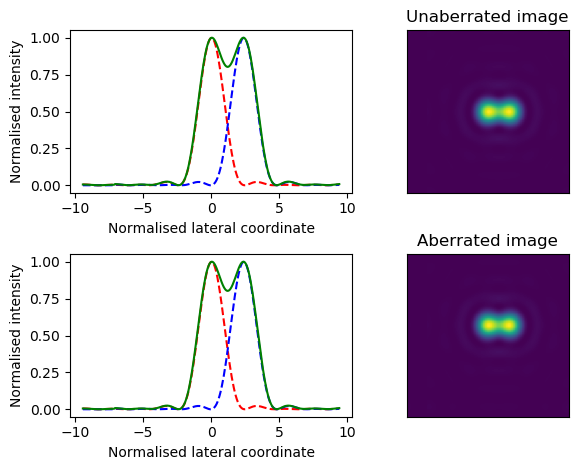
\includegraphics[width=\linewidth]{images/Airy_ring_2D_2_object_seperation_aberration_comparison_Noll_3.png}
		\caption{$rms(\Phi) = 1, \alpha_{1}^{1} = 1$}
		\label{fig:Airy_ring_2D_2_object_seperation_aberration_comparison_Noll_3}
	\end{subfigure}
	\begin{subfigure}{0.49\textwidth}
		\centering
		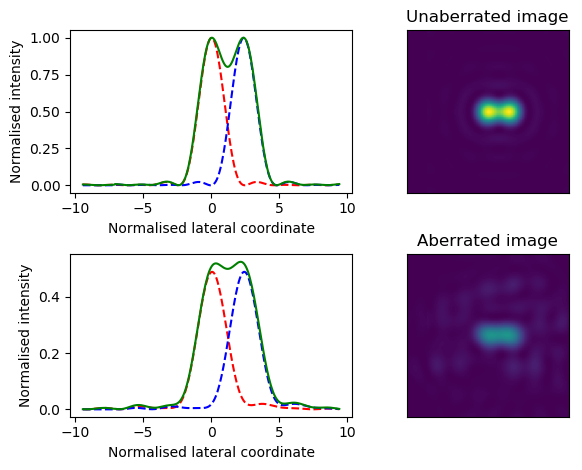
\includegraphics[width=\linewidth]{images/Airy_ring_2D_2_object_seperation_aberration_comparison_rms_1.png}
		\caption{$rms(\Phi) = 1$}
		\label{fig:Airy_ring_2D_2_object_seperation_aberration_comparison_rms_1}
	\end{subfigure}
	\caption[A visualisation of the effect of optical aberrations on image 
	resolution]{A visualisation of the effect of optical aberrations on 
		image resolution \textbf{(a)-(c)} Ideal diffraction limited point 
		sources at separation $r_{l}$ aberrated with $rms(\Phi) = 1$ of purely 
		piston, tip, and tilt respectively. \textbf{(d)} Ideal diffraction 
		limited point sources at separation $r_{l}$ aberrated with a random 
		phase distortion with $rms(\Phi) = 1$}
	\label{fig:aberrations_res}
\end{figure*}

\section{Adaptive Optics}
\label{sec:AO}

As previously mentioned, phase aberrations arise in microscopy primarily
due to heterogeneities in the structure of the biological sample being 
imaged. Consider the objective lens of a microscope. In the absence of
optical aberrations, as in Figure~\ref{fig:wavefront_focus_ideal}, a flat
wavefront is focused to a single diffraction limited spot. Introducing
a heterogeneous media distorts the phase wavefront and leads to an 
extended, non-diffraction limited focal spot as seen in 
Figure~\ref{fig:wavefront_focus_aberrated}. However, if, as in 
Figure~\ref{fig:wavefront_focus_corrected} the wavefront is not flat when 
it enters the microscope objective but instead shaped to compensate for 
the phase distortion, then an ideal, diffraction limited focal spot is 
recovered. Since the phase distortions encountered are not only sample
dependent, but spatially and (for live samples) temporally dependent an
adaptive method for pre-shaping the optical wavefront is 
required\cite{schwertner2004characterizing,wang2014multiplexed,girkin2009adaptive}.
The branch of technologies and methods for doing this is referred to as
adaptive optics (AO).

\begin{figure}[h]
	\centering
	\begin{subfigure}[t]{0.3\textwidth}
		\centering
		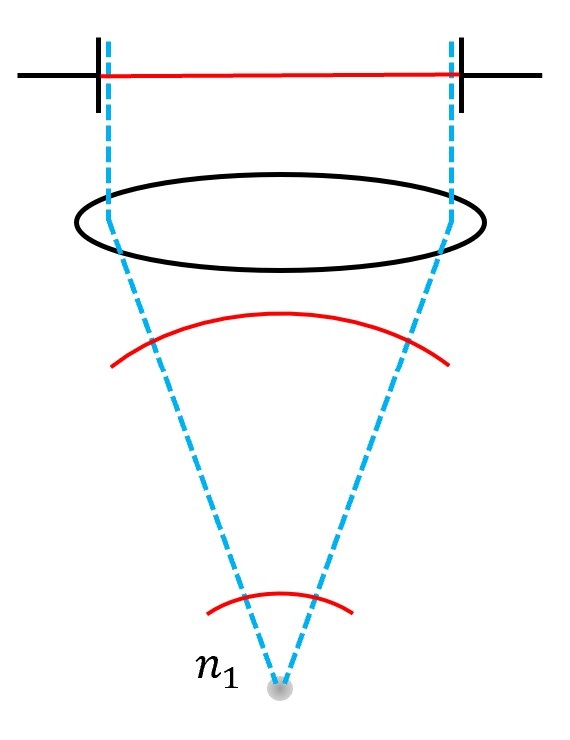
\includegraphics[width=\linewidth]{images/wavefront_focus_ideal.jpg}
		\caption{}
		\label{fig:wavefront_focus_ideal}
	\end{subfigure}
	\begin{subfigure}[t]{0.3\textwidth}
		\centering
		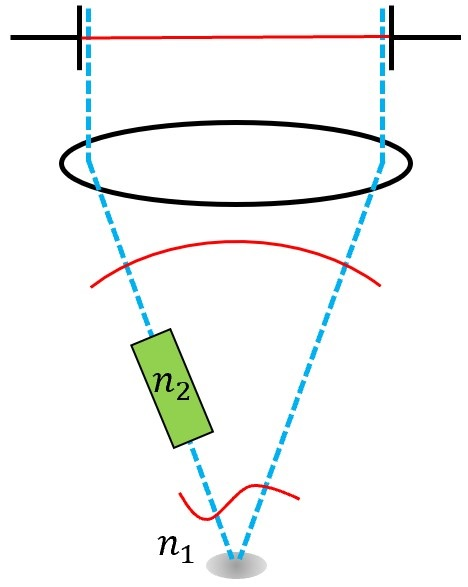
\includegraphics[width=\linewidth]{images/wavefront_focus_aberrated.jpg}
		\caption{}
		\label{fig:wavefront_focus_aberrated}
	\end{subfigure}
	\begin{subfigure}[t]{0.3\textwidth}
		\centering
		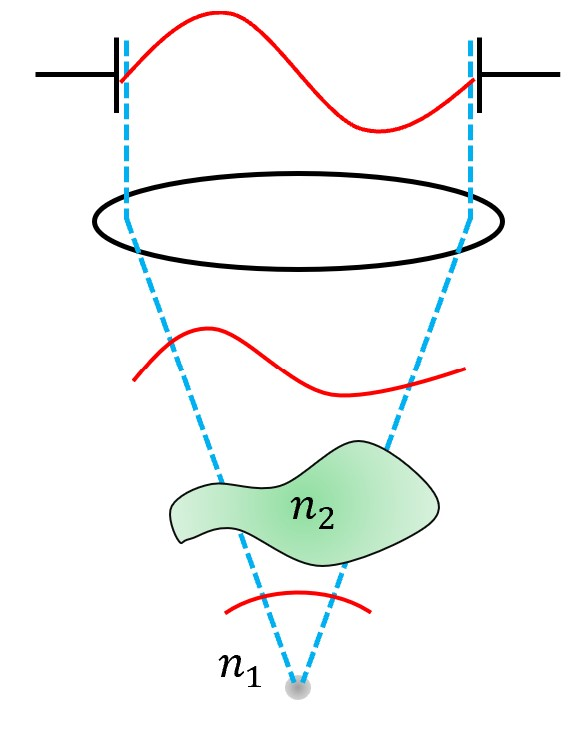
\includegraphics[width=\linewidth]{images/wavefront_focus_corrected.jpg}
		\caption{}
		\label{fig:wavefront_focus_corrected}
	\end{subfigure}
	\caption[Illustration of aberrations affecting a microscope objective focus.]{Illustration of aberrations affecting a microscope objective focus. \textbf{(a)} The microscope objective and surrounding media have the same refractive index, $n_{1}$ and the microscope objective forms a diffraction limited focal spot. \textbf{(b)} the media the wavefront passes through is heterogeneous. This causes a phase distortion in the wavefront and leads to an expanded focal spot. \textbf{(c)} Prior to the objective aperture, the wavefront is pre-shaped to the opposite shape to the expected distortion. Once the wavefront passes though the heterogeneous media, an ideal wavefront is recovered and thus the focal spot is diffraction limited again.}
	\label{fig:wavefront_focus}
\end{figure}

Similar to how the telescope and microscope have a shared historical origin,
the concept of using AO to correct for optical aberrations has it is 
origin in correcting for phase distortions in astronomical telescopes\cite{babcock1990adaptive}.
The principle of an AO system for microscopy is shown in 
Figure~\ref{fig:ao_system_schematic_simple}. Here, only the emission path 
is considered. A distorted wavefront $\Phi_{I}$, arrives at the aperture 
of the microscope. The wavefront is then imaged onto an adaptive element 
capable of applying a variable phase distortion, $\Phi_{AO}$. Once the 
wavefront has interacted with the adaptive element, there is a residual 
phase aberration $\Phi_{R} = \Phi_{I} - \Phi_{AO}$. 
Figure~\ref{fig:ao_system_schematic_simple} has the wavefront passing through
a beamsplitter and both being focused onto an imaging device and being 
directed to a wavefront sensor. In the latter case, $\Phi_{R}$ is 
calculated directly while in the former case $\Phi_{R}$ is inferred through 
some indirect measurement. Typically only one of these options is employed. 
The calculation of $\Phi_{R}$ is then passed to a controller which adjusts 
$\Phi_{AO}$ in order to minimise $rms(\Phi_{R})$. 
Figure~\ref{fig:ao_system_schematic_simple} assumes a reflective adaptive 
element such as a deformable mirror (DM) or a spatial light modulator (SLM), 
but the principles also apply for a transmissive adaptive element placed 
in the beam path, such as an opto-acoustic lens.

\begin{figure}[h]
	\centering
	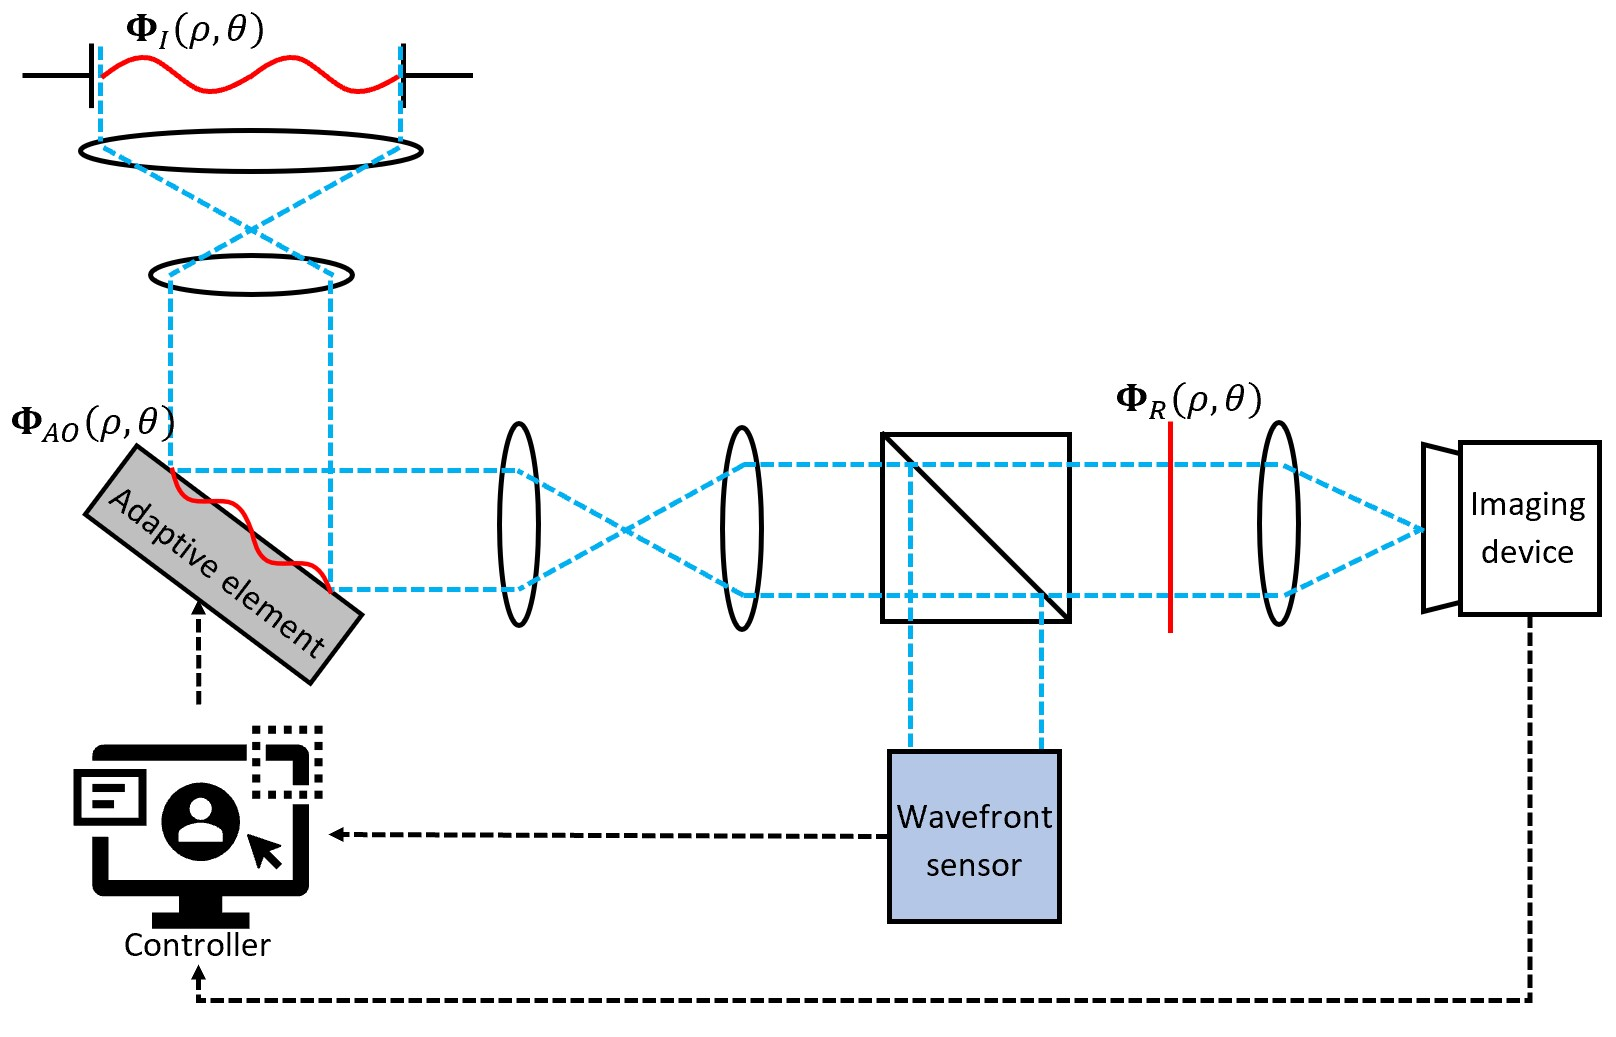
\includegraphics[width=\textwidth]{images/ao_system_schematic_simple.jpg}
	\caption[Schematic of the emission path of an adaptive optics system.]{Schematic of the emission path of an adaptive optics system. The emitted wavefront of a point in the fluorescent sample, $\Phi_{I}$, arrives at the aperture of the microscope. It is reimaged onto the adaptive element. The adaptive element has some phase, $\Phi_{AO}$, on its surface. The light then passed through a beamsplitter and is focused onto an imaging device. The residual phase aberration, $\Phi_{R} = \Phi_{I} - \Phi_{AO}$, is either calculated directly by the wavefront sensor or inferred indirectly from the data acquired by the imaging device. This information is passed to a controller which applies a phase aberration to the adaptive element, $\Phi_{AO}$, in order to minimise $rms(\Phi_{R})$.}
	\label{fig:ao_system_schematic_simple}
\end{figure}

Implementing AO in microscopy has already been shown to be highly 
effective at reducing optical aberrations and yielding significant 
improvements to image 
quality\cite{booth2014adaptive,girkin2009adaptive,fraisier2015adaptive,jesacher2011sensorless,
	jian2014wavefront}. Designing an AO enabled system follows a predicable 
workflow outlined in Figure~\ref{fig:ao_system_setup_workflow} 
consisting of four phases:

\begin{enumerate}
	\item \textit{System Design Phase}: A potential user should consider 
	the needs of their imaging modality, system constraints, desired 
	sample types before deciding on the appropriate AO element to 
	implement.
	\item \textit{Installation Phase}: The user installs the chosen AO 
	element into their beam path.
	\item \textit{Set-up Phase}: The AO element is calibrated to correct 
	for optical aberrations. This calibration is checked and the system 
	aberrations are corrected.
	\item \textit{Sample Correction Phase}: The sample correction routine 
	is designed. This will typically fall into one of two categories; 
	sensorless AO or direct wavefront sensing.
\end{enumerate}  

However, there are a number of adaptive elements\cite{olivier2002advanced}, 
a plethora of direct wavefront sensing techniques\cite{antonello2014optimisation,trumper2016instantaneous,
	schwertner2004measurement}, and wide array of 
sensorless correction methodologies\cite{burke2015adaptive,booth2002adaptive,
	fienup2003aberration,antonello2020multi,debarre2007image}. 
Considering AO within super-resolution imaging techniques further complicates
the 
situation\cite{debarre2008adaptive,booth2015aberrations,thomas2015enhanced}.
Since there is no universally agreed upon AO implementation, each 
implementation has to go through the entire design process from scratch, 
creating a bespoke but brittle implementation which is not easily transferable
to any other system, imaging modality, sample type, etc. 

\begin{figure}[h]
	\centering
	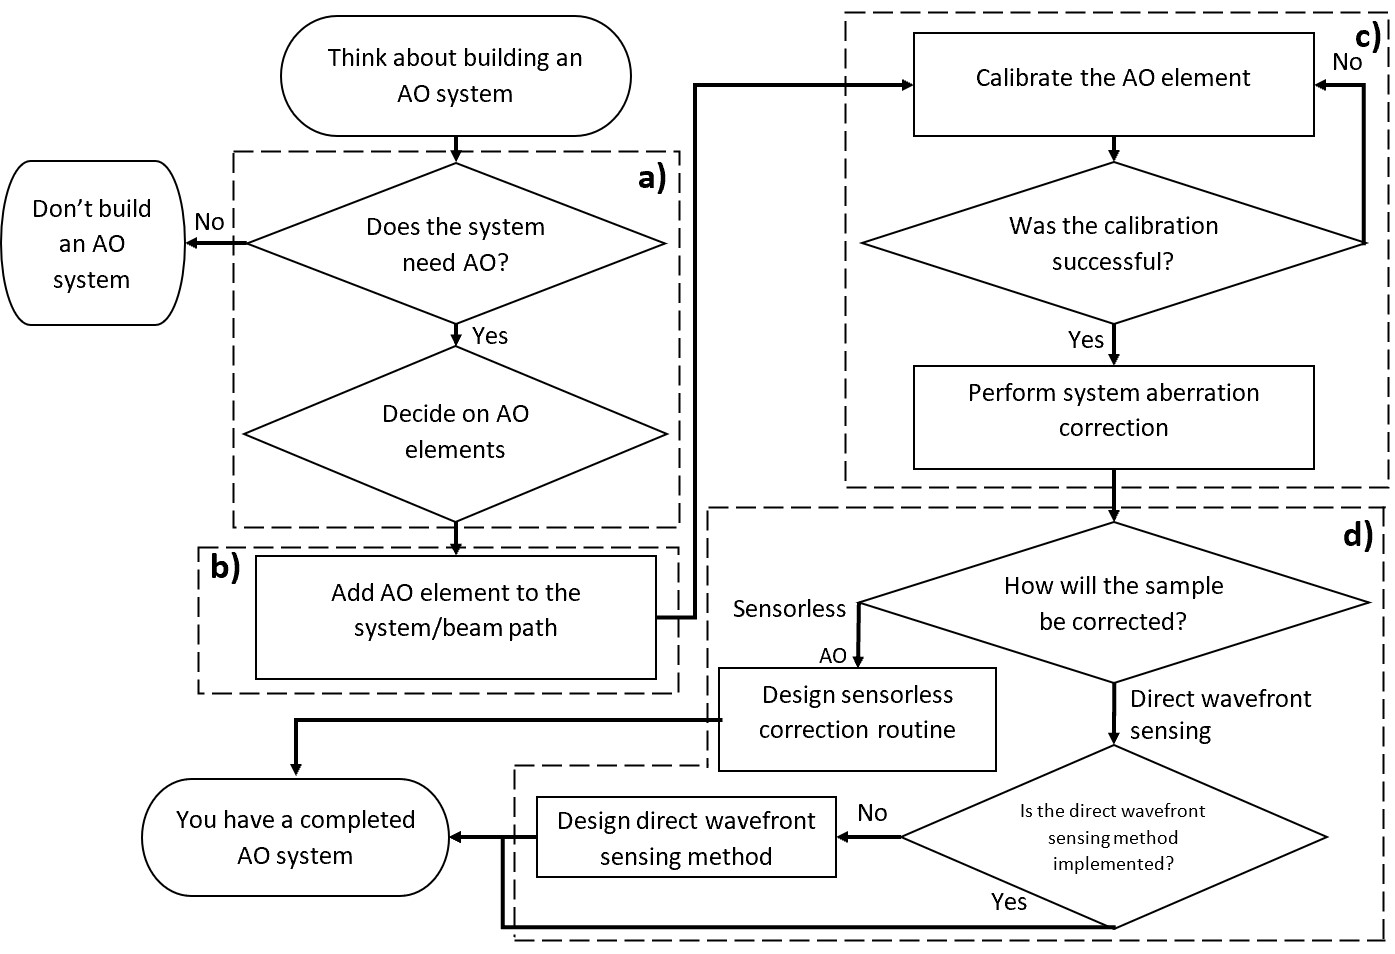
\includegraphics[width=1\textwidth, scale=0.5]{./images/ao_system_setup_workflow_new.jpg}
	\caption[Flowchart depicting the general process for building a system utilising AO.]{Flowchart depicting the general process for building a system utilising AO. \textbf{a)} \textit{System Design Phase}. User decides whether the system needs AO and, if so, what type. \textbf{b)} \textit{Installation Phase}. The chosen AO elements are added to the system. \textbf{c)} \textit{Set-up Phase}. The chosen AO element is calibrated. Typically, this involves mapping the variable elements of the AO element (e.g. deformable mirror actuators) to a useful set of basis functions which represent optical aberrations. \textbf{d)} \textit{Sample Correction Phase}. Here the user designs the methods to be used for correcting their desired sample.}
	\label{fig:ao_system_setup_workflow}
\end{figure}

\section{Overview and Aims of the Thesis}
\label{sec:overview}

There is a need for a robust, accurate, easy-to-use, general implementation 
of AO for microscopy\cite{ji2017adaptive,rodriguez2018adaptive}.
This implementation should be accessible to users in order to ensure its
adoption amongst the microscopy community and therefore the widespread 
adoption of AO technology. This thesis demonstrates just such an 
implementation - Microscope-AOtools - deployed successfully on two separate 
systems. The contributions of the thesis are collected into four chapters 
and is laid out as follows:

\begin{itemize}
	\item Chapter 2 discusses the two systems which Microscope-AOtools has
	been deployed on: Aurox Clarity and DeepSIM. It discusses their optical 
	layout and contains a brief discussion of the optical alignment 
	procedure as well as an alignment tool developed during the course of 
	this thesis; ``Hall, Nicholas J., David Miguel Susano Pinto, and Ian M. 
	Dobbie. "BeamDelta: simple alignment tool for optical systems." 
	\textit{Wellcome Open Research} 4.194 (2019): 194.''\cite{dobbie2019beamdelta} 
	The hardware control software - Python Microscope - used to synchronise 
	the disparate hardware elements of each microscope setup and the 
	graphical user interface (GUI) software - Microscope-Cockpit - which 
	is used to operate the microscopes are also discussed.
	\item Chapter 3 corresponds to scientific publication: ``Hall, Nicholas, 
	et al. ``Microscope-AOtools: A generalised adaptive optics 
	implementation.''
	\textit{Optics Express} 28.20 (2020): 28987-29003.''\cite{hall2020microscope}
	The generalised implentations of all the methods required by the Set-up and 
	Sample Correction phases detailed in Section~\ref{sec:AO} are discussed.
	It also contains discussion of the integration of Microscope-AOtools with
	Microscope-Cockpit in order to enable accessibility for users.
	\item Chapter 4 corresponds to the scientific publication: ``Hussain, 
	Syed Asad, et al. ``Wavefront-sensorless adaptive optics with a 
	laser-free spinning disk confocal microscope.'' \textit{Journal of 
		Microscopy} (2020).'' 
	on which the author is a co-first author\cite{hussain2020wavefront}. It details the successful 
	implementation of Microscope-AOtools on the Aurox Clarity system.
	\item Chapter 5 details the successful implementation of Microscope-AOtools 
	on the DeepSIM system. The results and implementation presented here will
	contribute significantly to a future publication of the DeepSIM system.
\end{itemize}

Discussions of existing limitations and areas for further development to the 
presented AO implementation are presented in Chapter 6. Conclusions are drawn 
in Chapter 7. The Aurox Clarity system was built by Dr Syed Hussain of the 
Dynamic Optics and Photonics Group, University of Oxford and Toshiki Kubo
Department of Applied Physics, Osaka University. The design and original 
implementation of the DeepSIM system was built by Dr Ian Dobbie, Dr Mick 
Philips, Dr Antonia G\"{o}hler and Dr Mantas \v{Z}urauskas, 
all members of the Micron Advanced Imaging Consortium at the time. The author 
implemented a number of modifications, improvements, and realignments in 
order to produce the demonstrations shown in this thesis.
\chapter{Methods and Implementations}

\section{DeepSIM}
\label{sec:DeepSIM}

\begin{itemize}
	\item This is the system that the bulk of the data is/will be collected from so it's important to explain the components of it.
\end{itemize}

	\subsection{DeepSIM Optical Set-up}
	\label{subsec:DeepSIM_optics}
	
	\begin{itemize}
		\item Explain dual beam paths, multiple lasers with the same exit point, etc.
		\item Explain interferometric path for direct wavefront sensing and why it's preferred over Shack-Hartmann.
	\end{itemize}

	\subsection{Optical Alignment}
	\label{subsec:alignment}
	
	\begin{itemize}
		\item Here's an opportunity to talk about BeamDelta and the need to minimise optical misalignment as DMs (and  AO components in general) cannot offer infinite correction so you still want a well algined system you do minor corrections than a poorly aligned system that you can't fully correct.
	\end{itemize}

	\subsection{\textit{Microscope}}
	\label{subsec:microscope}
	
	\begin{itemize}
		\item Talk about the need for hardware control in bespoke microscope systems and for precise, coordinated timing control.
	\end{itemize}

	\subsection{\textit{Cockpit}}
	\label{subsec:cockpit}
	
	\begin{itemize}
		\item Here need to talk about having an accessible interface for biologist to use.
		\item Mention peculiarities with DeepSIM (i.e. no eye pieces) and call back to the previous inaccessibly of AO to biologists due to complex interfaces.
	\end{itemize}

\section{Adaptive Optics Control Software}
\label{sec:AOtools}

Implementing adaptive optics (AO) in microscopy has already been shown to be highly effective at removing optical aberrations and yielding significantly improvements to image quality.\cite{booth2014adaptive,girkin2009adaptive} However, AO technology has not been widely adopted due to a number of barriers. Firstly, it is not trivial to set-up an AO element such as the deformable mirror (DM) present in the DeepSIM optical path. The DM must be calibrated to meaningfully recreate and correct aberrations, but performing this step is not something non-specialist user may know how to do or how to assess if the process has been successful.vSecondly, measuring the wavefront deformations (and therefore the aberrations) present in a sample is complicated. While direct wavefront measurements do exits, they carry additional complications and are only applicable in certain samples.\cite{wang2014rapid,wang2015direct} Therefore indirect wavefront sensing is generally preferred which requires inferring the aberrations present from the variance of a measure of the image quality.\cite{rodriguez2018adaptive} This adds an additional complication since there is no universal image quality metric. Indeed, they often vary between sample type and imaging modality.\cite{burke2015adaptive,booth2002adaptive,fienup2003aberration,debarre2008adaptive} For these reasons, a robust, easy-to-use implementation which incorporates multiple AO methods for multiple sample types/imaging modalities has yet to be presented.\cite{ji2017adaptive}

Microscope-AOtools provides such an implementation, utilising Python Microscope to provide control over the physical hardware. It incorporates methods for calibrating a DM, evaluating the success of the calibration in recreating aberrations and performing both direct wavefront sensing and sensorless adaptive optics corrections. The methods for sensorless adaptive optics correction can utilise a number from a suite of image quality metrics which can be easily extended to include additional sample or imaging method-specific metrics. These methods are automated, require minimal user involvement and setup and are tied to simple, descriptive  buttons on the Cockpit UI allowing for greater accessibility to users, shown in Figure~\ref{fig:Cockpit_UI}. The overall UI presented to users of DeepSIM is shown in Figure~\ref{fig:DeepSIM_control_software} and the functions specific to the DM are shown in Figure~\ref{fig:DM_methods_cockpit}. These methods are divided into two categories; Set-up methods and Use-case methods.

\begin{figure}[h]
	\centering
	\begin{subfigure}{0.45\textwidth}
		\centering
		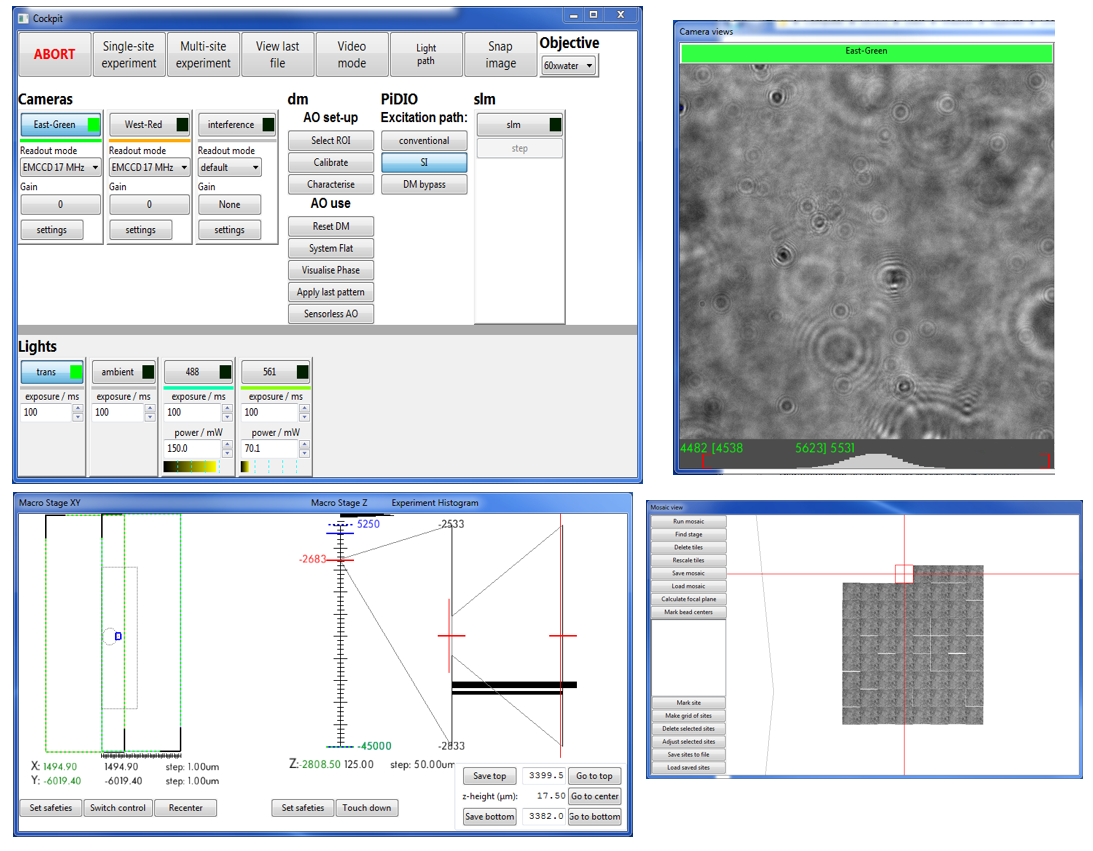
\includegraphics[width=1\linewidth, scale=0.5]{images/DeepSIM_control_software.png}
		\caption{}
		\label{fig:DeepSIM_control_software}
	\end{subfigure}
	\begin{subfigure}{0.45\textwidth}
		\centering
		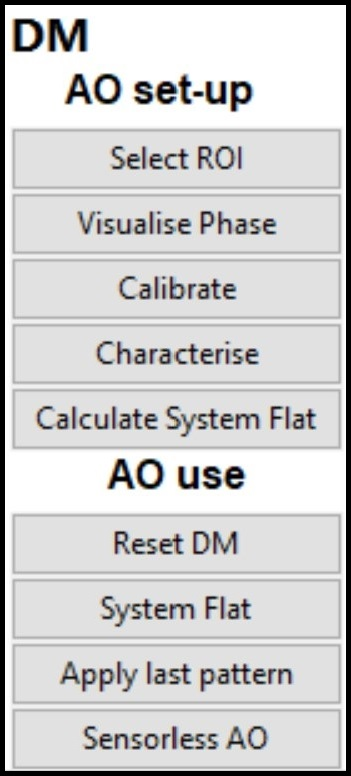
\includegraphics[width=0.35\linewidth, scale=0.5]{images/DM_methods_cockpit.jpg}
		\caption{}
		\label{fig:DM_methods_cockpit}
	\end{subfigure}
	\caption{(a) Cockpit UI for controlling DeepSIM (b) Deformable mirror specific functions on the Cockpit UI}
	\label{fig:Cockpit_UI}
\end{figure}

\subsection{Set-up Methods}
\label{subsec:set_up_methods}

As previously described, DeepSIM has multiple beam paths; interferometric, widefield and SIM. The interferometric beampath is used for calibrating the deformable mirror. The interferometric image is formed by the interference between the reference beam arm and the system beam arm. However due to differences in magnification, the size of the reference beam is larger than that of the system beam. Therefore it is necessary to have a method for selecting the interferometric region of interest (ROI) i.e. the region where the reference and system beam arms interfere. Cockpit implements such a method as the functionality of the "Select ROI" button shown in Figure~\ref{fig:DM_methods_cockpit}. This spawns the windown shown in Figure~\ref{fig:ROI_selectors} where the user can draw a circle which will define the inferferometric ROI. This coordinates of this ROI are saved to the microscope's configuration files with the "Save ROI" button.

\begin{figure}[h]
	\centering
	\begin{subfigure}{0.4\textwidth}
		\centering
		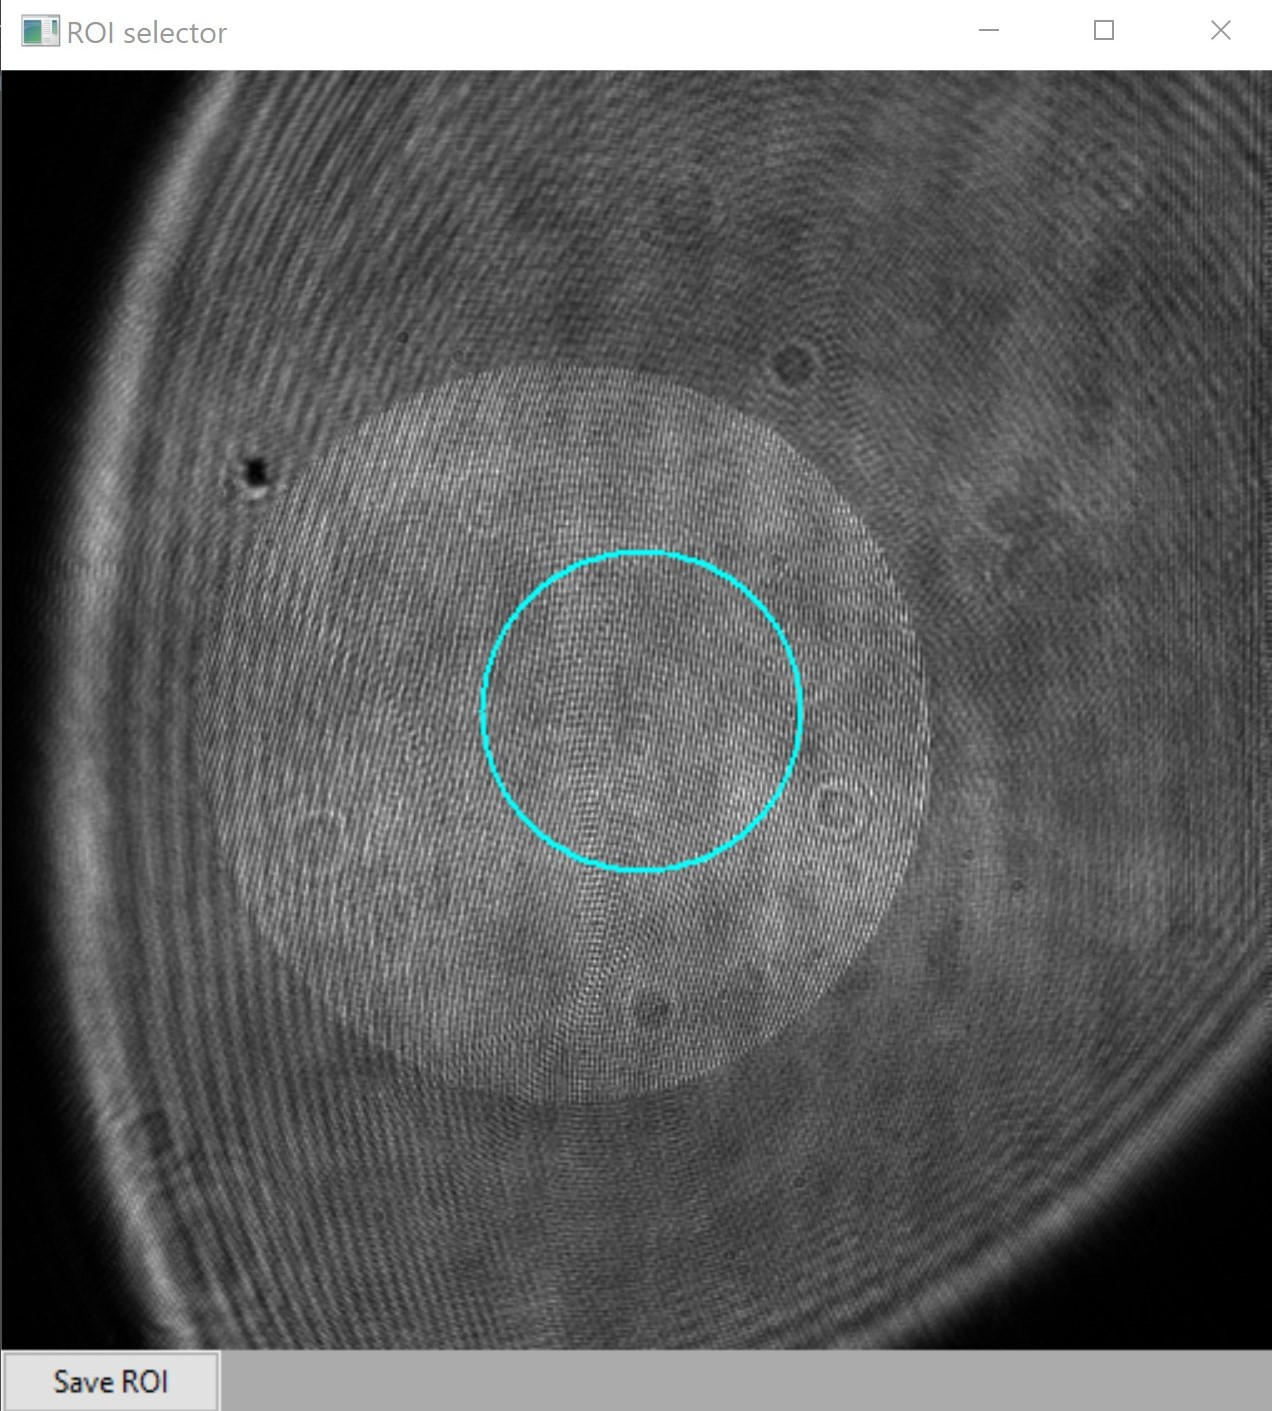
\includegraphics[width=1\linewidth]{images/ROI_selector_init.jpg}
		\caption{}
		\label{fig:ROI_selector_init}
	\end{subfigure}
	\begin{subfigure}{0.4\textwidth}
		\centering
		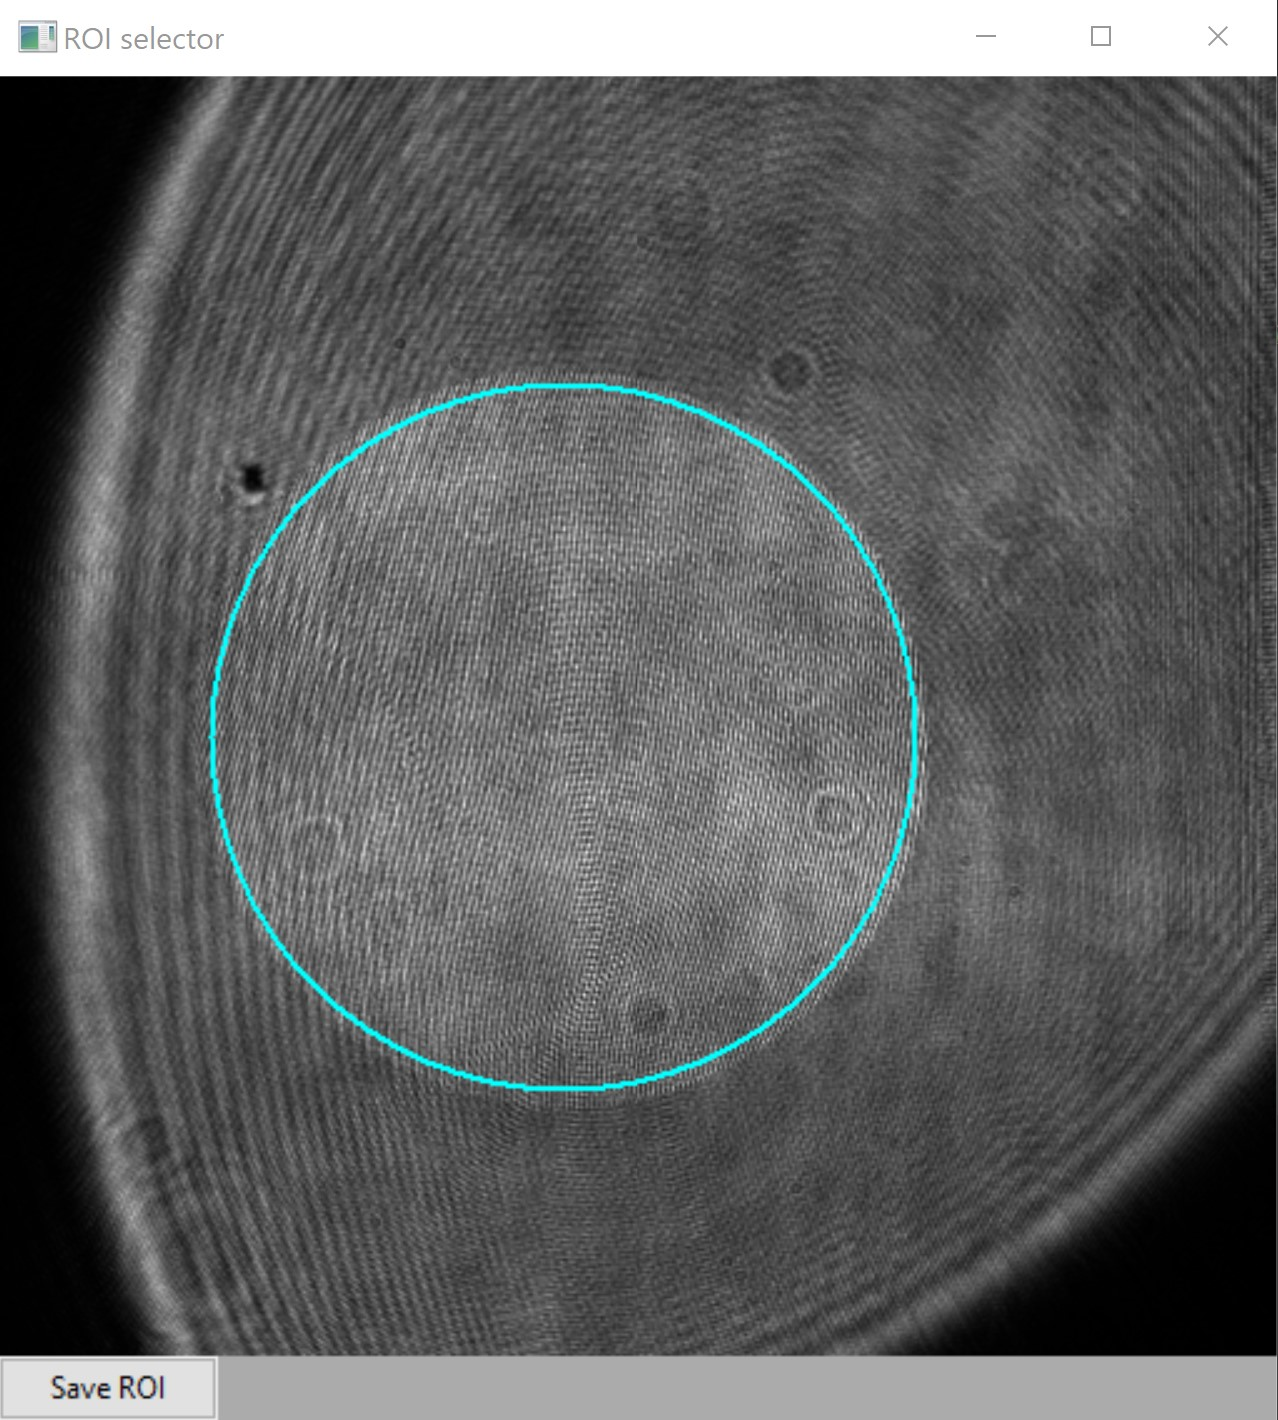
\includegraphics[width=1\linewidth]{images/ROI_selector.jpg}
		\caption{}
		\label{fig:ROI_selector}
	\end{subfigure}
	\caption{User interface for selecting the interferometric region of interest (a) The ROI selecter UI when it is first initialised (b) UI with the ROI selected}
	\label{fig:ROI_selectors}
\end{figure}

\subsubsection{Direct wavefront sensing}
\label{subsubsec:direct_wavefront_sensing}

The two most common methods for direct wavefront sensing are Shack-Hartmann and interferometric methods. Shack-Hartmann wavefront sensing is useful for instances where accuracy is less important than the speed of wavefront recovery. While these situations do exist, the current use-cases for direct wavefront sensing within DeepSIM and Microscope-AOtools are calibration and system aberration correction. These are both situation where accuracy is considerably more important than speed. Additionally, implementing phase extraction from interferometric data has proved more challenging  to implement in an automatic fashion. Interferometric data can be defined as:

\begin{equation}\label{eq:I_basic}
I(x,y,t) = a(x,y) + b(x,y)cos[\phi(x,y) + \Phi_{R}(x,y,t)]
\end{equation}

Where $a(x,y)$ describes the variation of the background illumination, $b(x,y)$ describes the noise and contrast variations, $\phi(x,y)$ describes the phase imparted by the DM surface and $\Phi_{R}(x,y,t)$ is the reference phase at time $t$. $\Phi_{R}(x,y,t)$ can be arbitrarily set to 0. Doing this and then expanding the cosine term using Euler's formula, as well as the definition that $c(x,y) = \frac{1}{2}b(x,y)e^{i\phi(x,y)}$ leads to:

\begin{equation}\label{eq:I_cos_expand}
I(x,y) = a(x,y) + c(x,y) + c^{*}(x,y)
\end{equation}

Applying the 2-D Fourier transform Equation~\ref{eq:I_cos_expand} becomes:

\begin{equation}\label{eq:I_fourier}
\boldsymbol{I}(u,v) = \boldsymbol{A}(u,v) + \boldsymbol{C}(u,v) + \boldsymbol{C}^{*}(u,v)
\end{equation}

Now, given that $I(x,y)$ is real valued, it naturally follows that $\boldsymbol{I}(u,v)$ is Hermitian. The amplitude spectrum is symmetric around the zero position (i.e. $u = 0$, $v = 0$). This means that $\boldsymbol{C}(u,v)$ and $\boldsymbol{C}^{*}(u,v)$ must contain the same information, only centred on different spatial frequencies. One can apply a bandpass filter in the spatial frequency domain to remove both $\boldsymbol{A}(u,v)$ and $\boldsymbol{C}^{*}(u,v)$ to leave only $\boldsymbol{C}(u,v)$.\cite{lewis1993absolute} Applying the inverse Fourier transform yields $c(x,y)$, which is now complex. The phase of the wavefront can then be recovered by:

\begin{equation}\label{eq:phase}
\phi(x,y) = \arctan \frac{\Im\{c(x,y)\}}{\Re\{c(x,y)\}}
\end{equation}

In the phase unwrapping workflow shown in Figure~\ref{fig:phase_unwrap_workflow}, these mathematical steps are implemented in a practical way. The interferogram (\ref{fig:puw_inteferogram}) is cropped (\ref{fig:puw_inteferogram_cropped}) and the ROI, that is the area described by Equation~\ref{eq:I_basic}, is isolated by masking out all the information outside the ROI. This is provided by the user using the ROI selector shown in Figure~\ref{fig:ROI_selector}. Quadrant shifting the image (\ref{fig:puw_data_fftshift}) and applying a tukey window mask (\ref{fig:puw_tukey_window}) is done to minimise the spurious spatial frequencies which arise from performing a fast Fourier transform (FFT) on an image with sharp discontinuities at the quadrant edges.

\begin{figure*}
	\centering
	\begin{subfigure}{0.23\textwidth}
		\centering
		\includegraphics[width=1\linewidth, scale=0.5]{images/puw_inteferogram.png}
		\caption{}
		\label{fig:puw_inteferogram}
	\end{subfigure}
	\begin{subfigure}{0.23\textwidth}
		\centering
		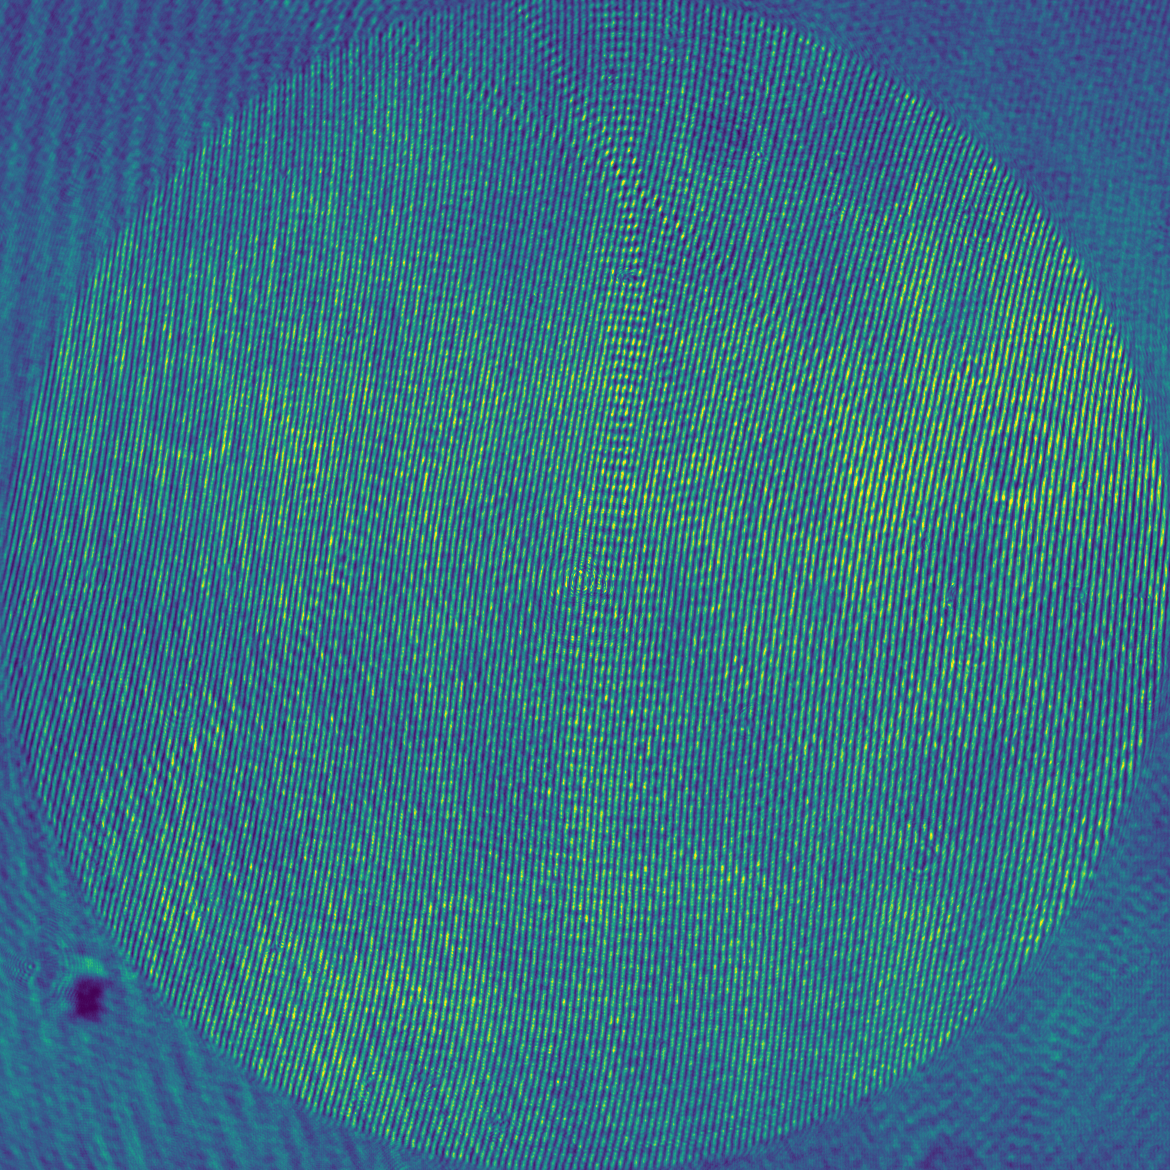
\includegraphics[width=1\linewidth, scale=0.5]{images/puw_inteferogram_cropped.png}
		\caption{}
		\label{fig:puw_inteferogram_cropped}
	\end{subfigure}
	\begin{subfigure}{0.23\textwidth}
		\centering
		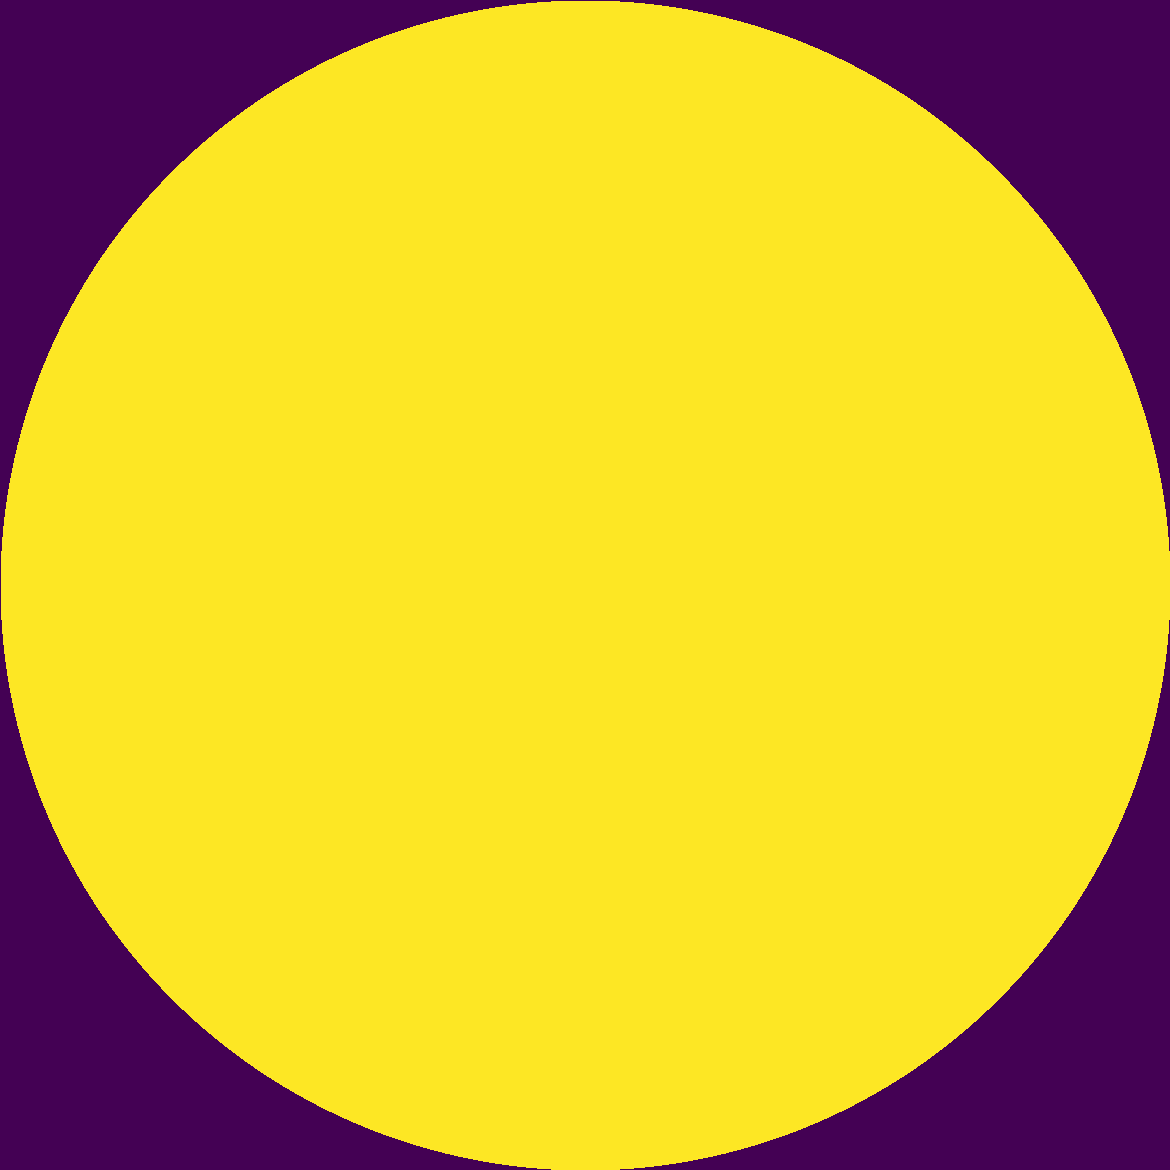
\includegraphics[width=1\linewidth, scale=0.5]{images/puw_mask.png}
		\caption{}
		\label{fig:puw_mask}
	\end{subfigure}
	\begin{subfigure}{0.23\textwidth}
		\centering
		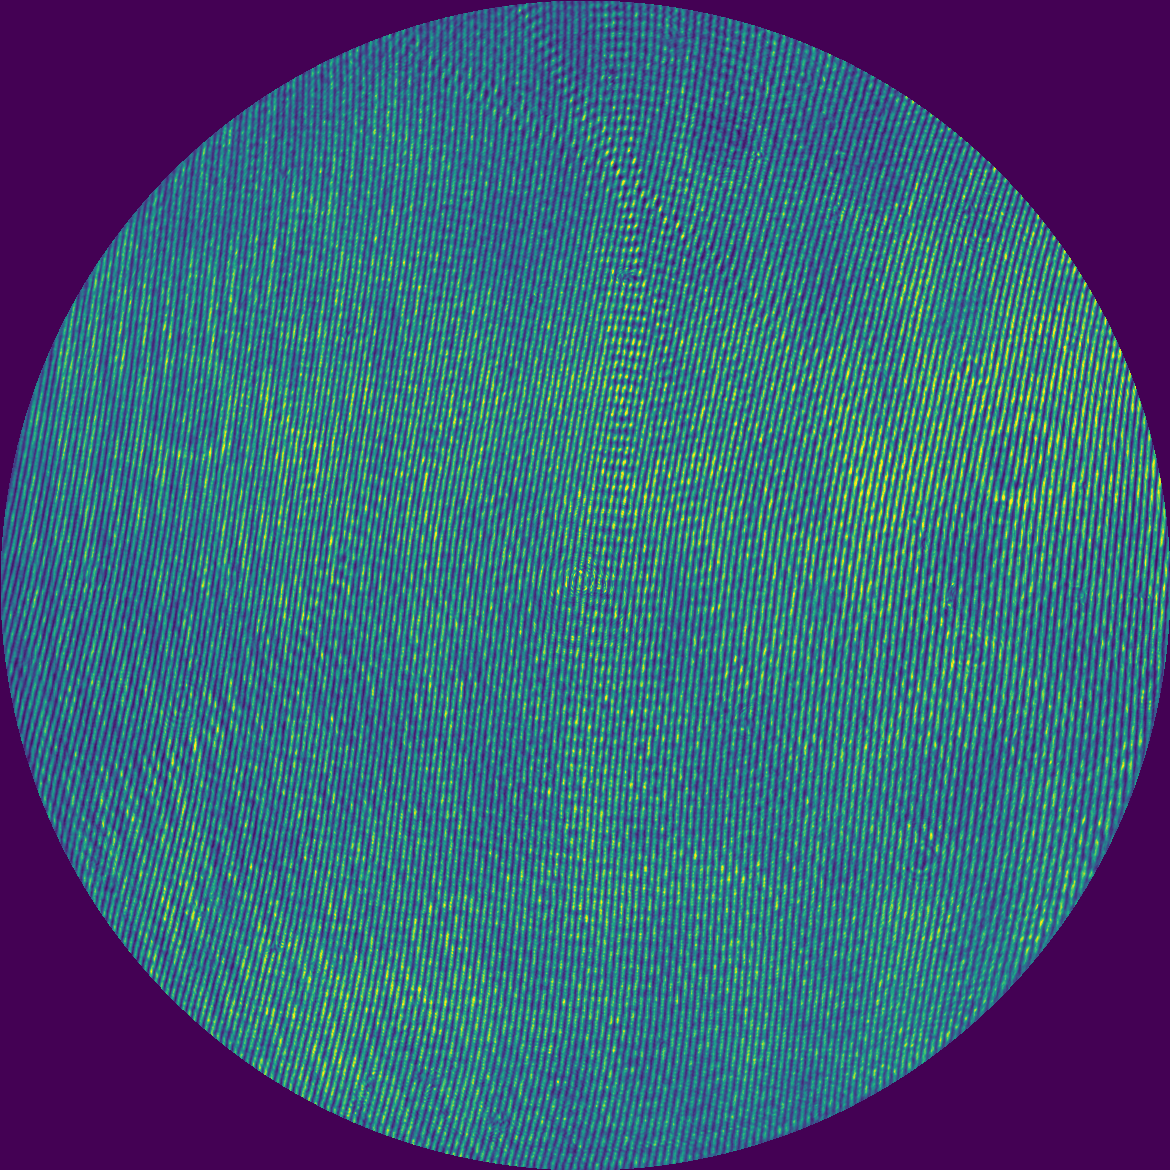
\includegraphics[width=1\linewidth, scale=0.5]{images/puw_data_masked.png}
		\caption{}
		\label{fig:puw_data_masked}
	\end{subfigure}
	
	\begin{subfigure}{0.23\textwidth}
		\centering
		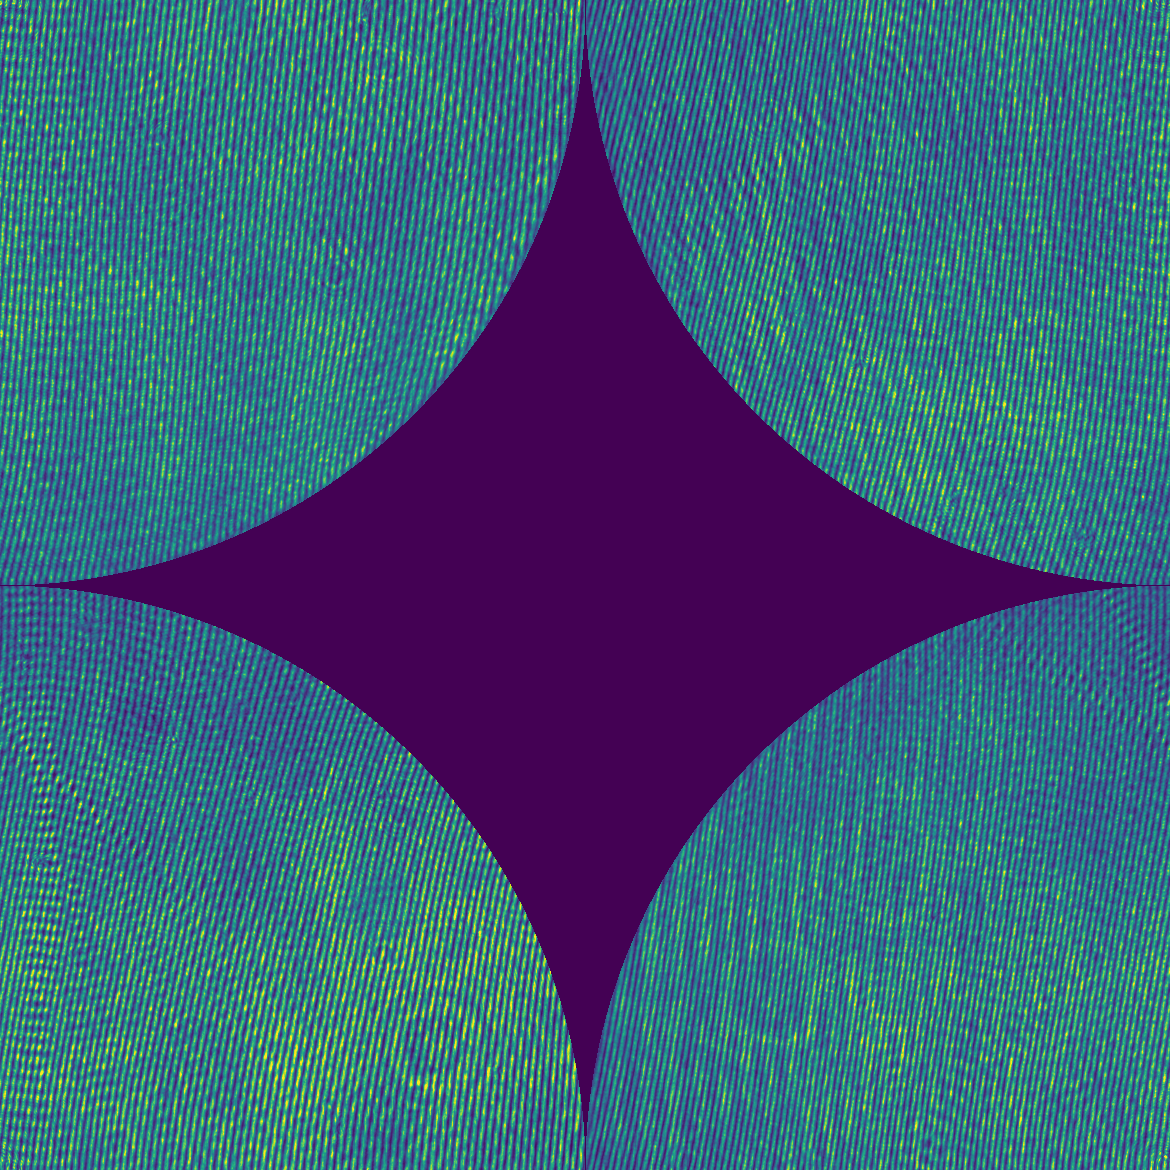
\includegraphics[width=1\linewidth, scale=0.5]{images/puw_data_fftshift.png}
		\caption{}
		\label{fig:puw_data_fftshift}
	\end{subfigure}
	\begin{subfigure}{0.23\textwidth}
		\centering
		
\includegraphics[width=1\linewidth, scale=0.5]{images/puw_tukey_window.png}
		\caption{}
		\label{fig:puw_tukey_window}
	\end{subfigure}
	\begin{subfigure}{0.23\textwidth}
		\centering
		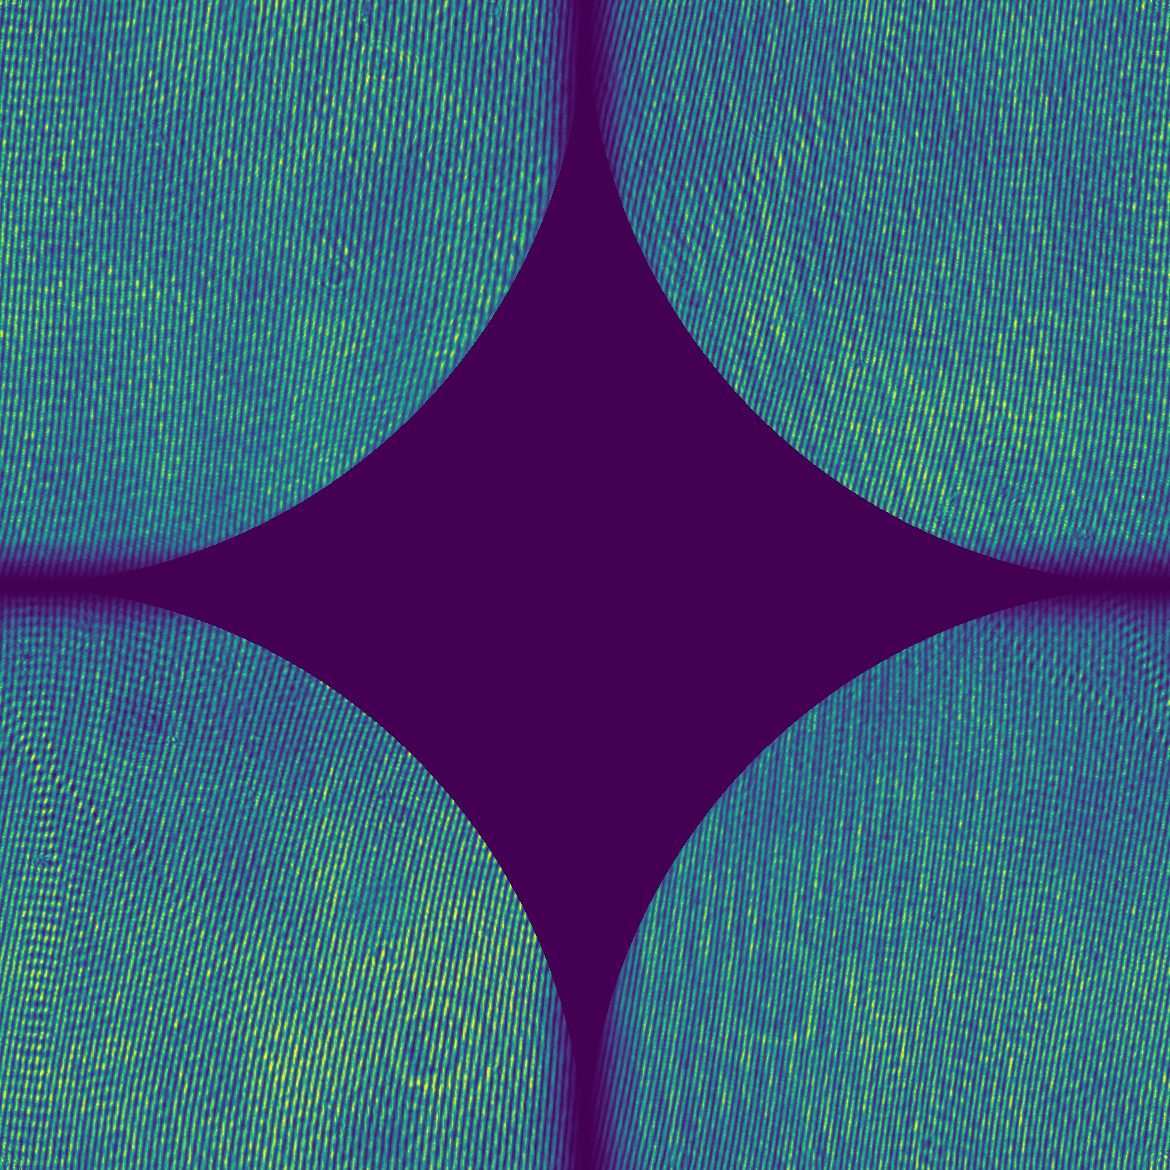
\includegraphics[width=1\linewidth, scale=0.5]{images/puw_fringes_tukey.png}
		\caption{}
		\label{fig:puw_fringes_tukey}
	\end{subfigure}
	\begin{subfigure}{0.23\textwidth}
		\centering
		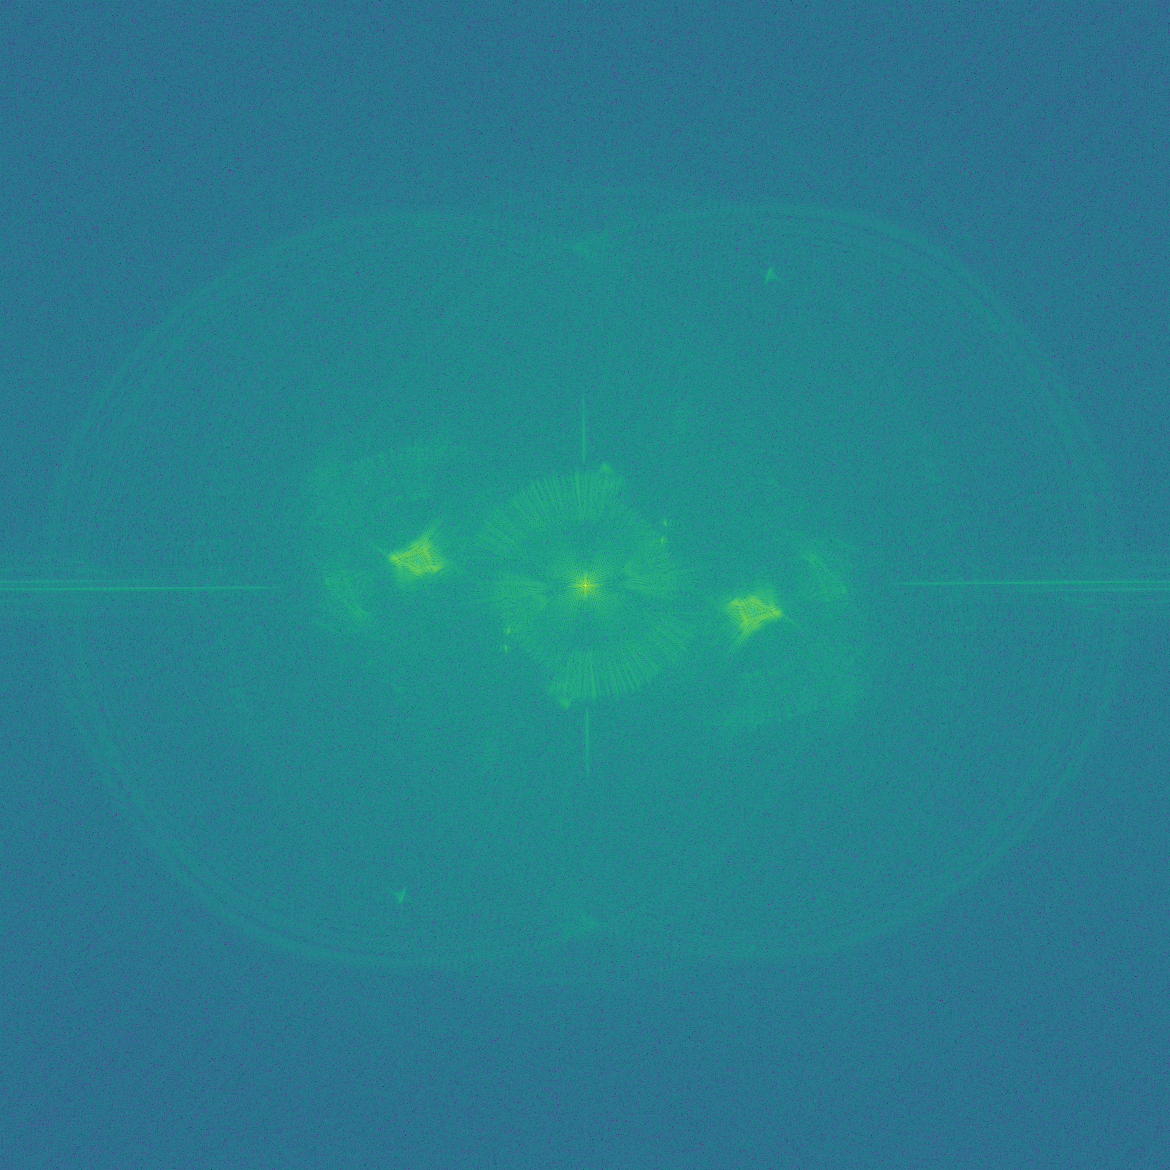
\includegraphics[width=1\linewidth, scale=0.5]{images/puw_new_fringe_fft.png}
		\caption{}
		\label{fig:puw_new_fringe_fft}
	\end{subfigure}
	
	\begin{subfigure}{0.23\textwidth}
		\centering
		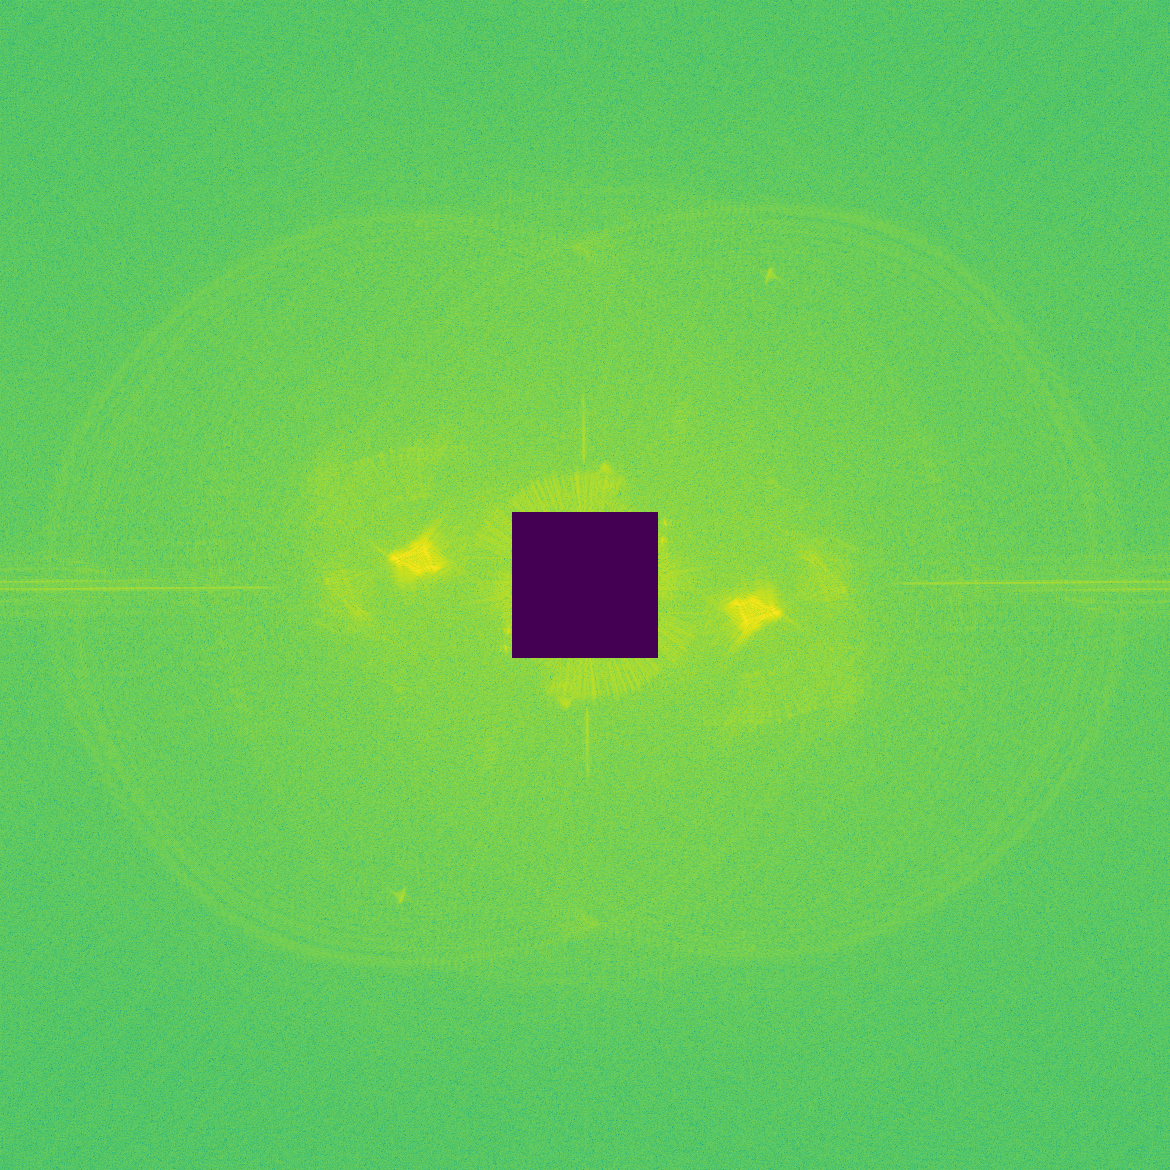
\includegraphics[width=1\linewidth, scale=0.5]{images/puw_new_fringe_fft_centre_blocked.png}
		\caption{}
		\label{fig:puw_new_fringe_fft_centre_blocked}
	\end{subfigure}
	\begin{subfigure}{0.23\textwidth}
		\centering
		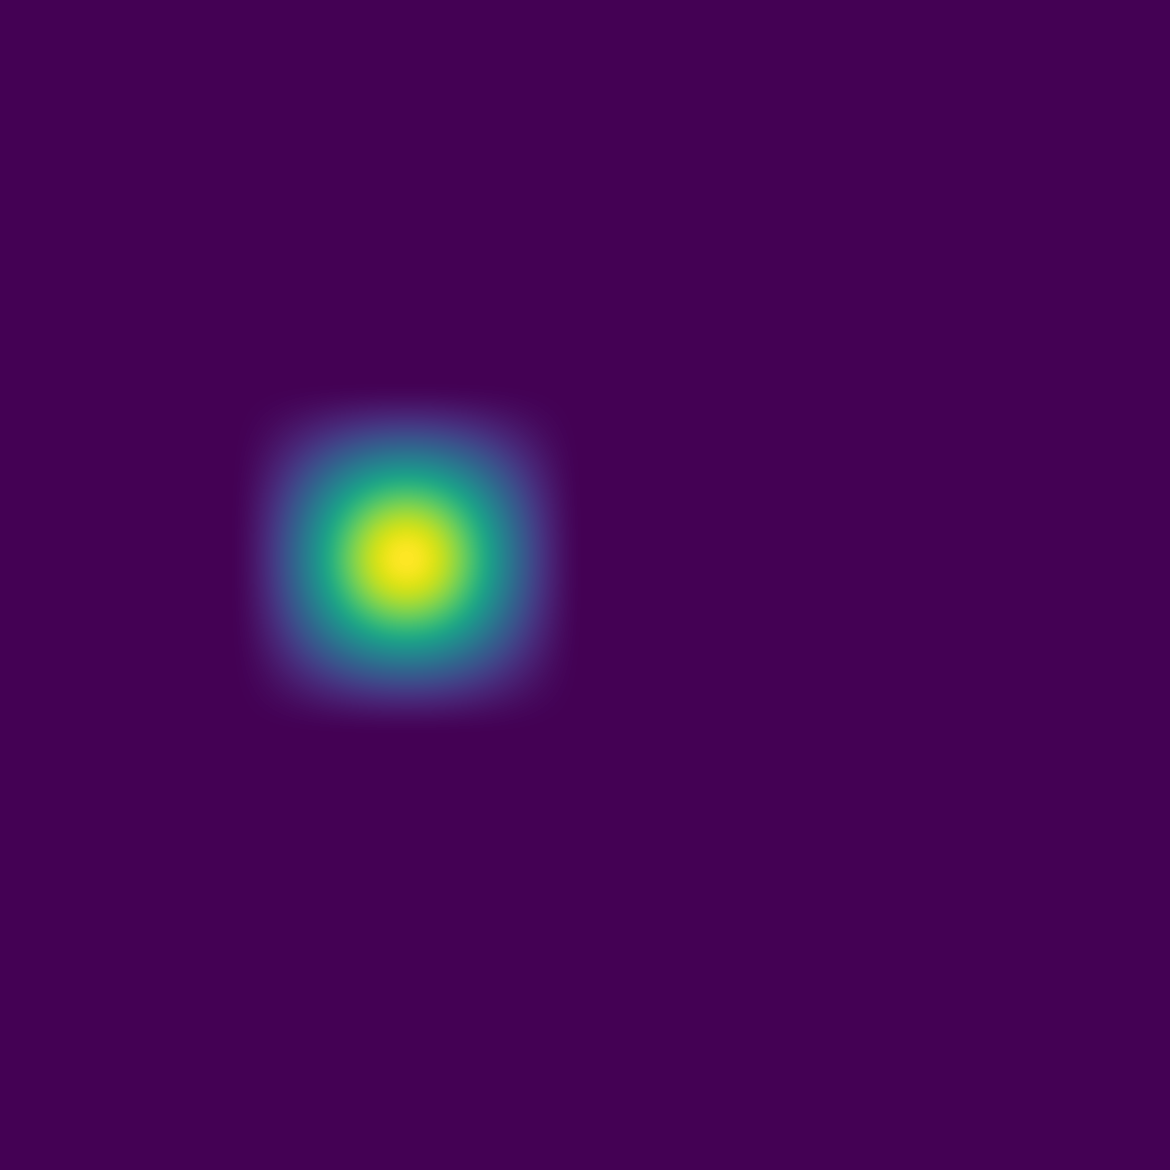
\includegraphics[width=1\linewidth, scale=0.5]{images/puw_fft_filter.png}
		\caption{}
		\label{fig:puw_fft_filter}
	\end{subfigure}
	\begin{subfigure}{0.23\textwidth}
		\centering
		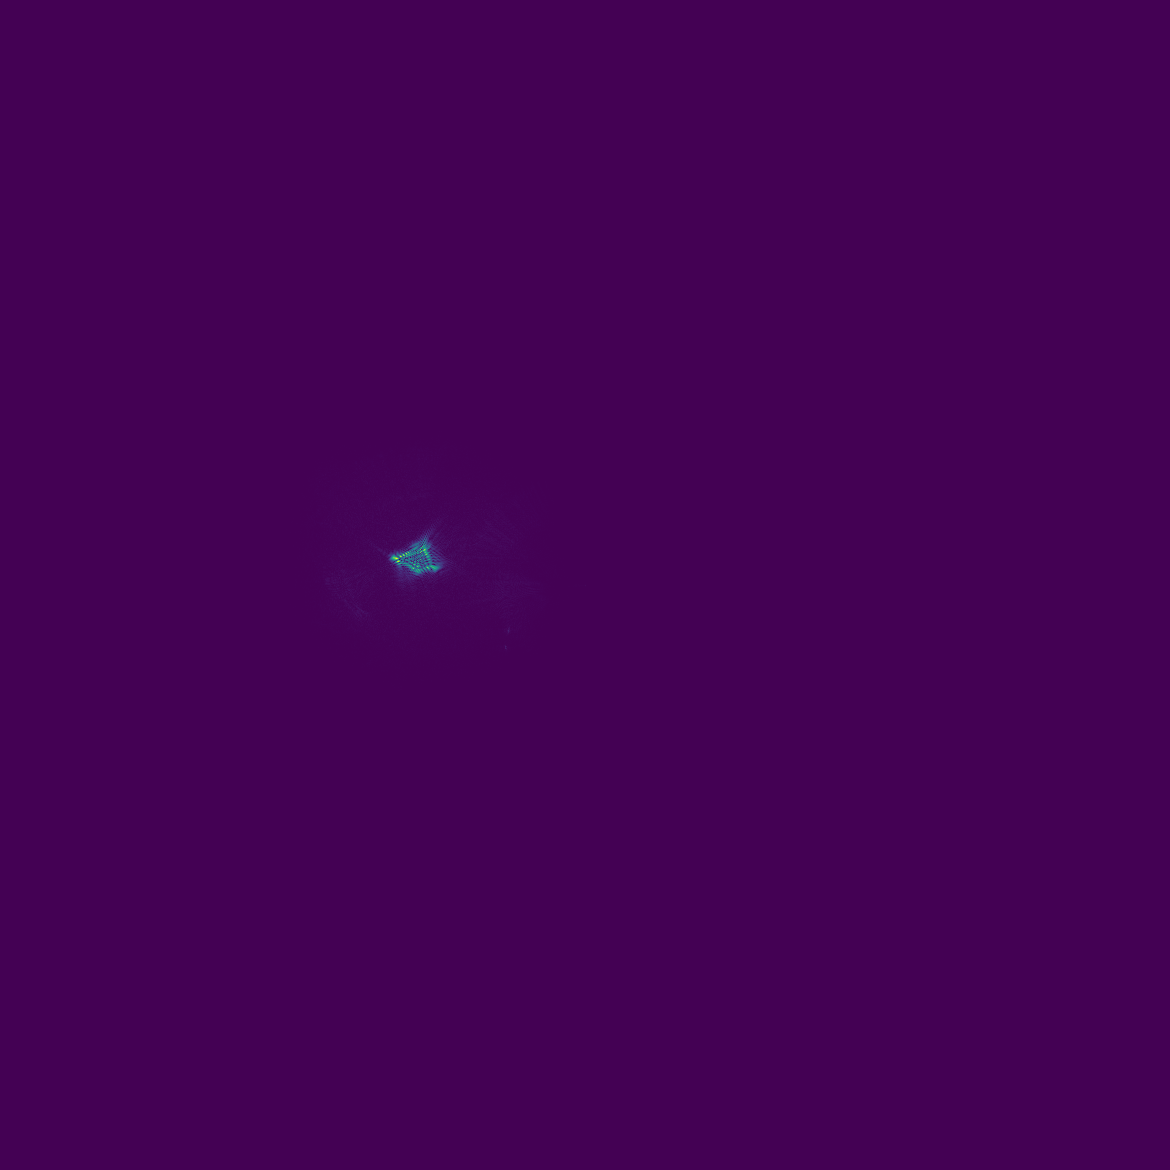
\includegraphics[width=1\linewidth, scale=0.5]{images/puw_new_fringe_order1.png}
		\caption{}
		\label{fig:puw_new_fringe_order1}
	\end{subfigure}
	\begin{subfigure}{0.23\textwidth}
		\centering
		\includegraphics[width=1\linewidth, scale=0.5]{images/puw_order1_roll.png}
		\caption{}
		\label{fig:puw_order1_roll}
	\end{subfigure}
	
	\begin{subfigure}{0.23\textwidth}
		\centering
		\includegraphics[width=1\linewidth, scale=0.5]{images/puw_complex_phase.png}
		\caption{}
		\label{fig:puw_complex_phase}
	\end{subfigure}
	\begin{subfigure}{0.23\textwidth}
		\centering
		\includegraphics[width=1\linewidth, scale=0.5]{images/puw_phaseorder1.png}
		\caption{}
		\label{fig:puw_phaseorder1}
	\end{subfigure}
	\begin{subfigure}{0.23\textwidth}
		\centering
		\includegraphics[width=1\linewidth, scale=0.5]{images/puw_phaseorder1mask}
		\caption{}
		\label{fig:puw_phaseorder1mask}
	\end{subfigure}
	\begin{subfigure}{0.23\textwidth}
		\centering
		\includegraphics[width=1\linewidth, scale=0.5]{images/puw_unwrapped_phase.png}
		\caption{}
		\label{fig:puw_unwrapped_phase}
	\end{subfigure}
	\caption{A visualisation of the stages of the phase unwrap workflow. (a) Captured interferogram (b) Interferogram cropped to region of interest (ROI) (c) Circular mask (d) ROI isolated (e) ROI quadrant shifted (ROI-qs) (f) 2-D tukey window mask (g) ROI-qs with tukey mask applied (h) Fast Fourier transform (FFT) of (g), log scaled (i) Fourier transform with the central spatial frequencies masked, log scaled (j) 2-D sine squared mask centred on the position of spatial frequencies encoding the phase information (k) The original Fourier transform, (h), with the sine squared mask applied (l) Phase encoding spatial frequencies rolled to the central position (m) Inverse FFT of the phase encoding spatial frequencies (n) Inverse FFT transformed into a phase map (o) Phase map masked to isolate ROI (p) Phase map unwrapped to remove 2$\pi$ discontinuities}
	\label{fig:phase_unwrap_workflow}
\end{figure*}

Having performed the FFT (\ref{fig:puw_new_fringe_fft}), an array described by Equation~\ref{eq:I_fourier} is obtained. A selection of the central spatial frequencies are masked (\ref{fig:puw_new_fringe_fft_centre_blocked}), primarily to mask out the central spatial frequency which represents the mean intensity and has an amplitude orders of magnitude larger than any other spatial frequency. The spatial frequencies which now have the highest amplitudes correspond to both $\boldsymbol{C}(u,v)$ and $\boldsymbol{C}^{*}(u,v)$. One of the aforementioned amplitude peaks is located and a bandpass filter described by $\sin^{2}(x,y)$ is constructed (\ref{fig:puw_fft_filter}) centred on the spatial frequency location of this amplitude peak. As previously noted, the Fourier transform of the interferogram is symmetrical around the central spatial frequency. So, it doesn't matter which of the two peaks this filter is centred on since they encode the same information. This bandpass filter is then applied to the FFT of the interferogram (\ref{fig:puw_new_fringe_order1}) and these spatial frequencies are then rolled to the central spatial frequency position (\ref{fig:puw_order1_roll}). This successfully filters $\boldsymbol{A}(u,v)$ and $\boldsymbol{C}^{*}(u,v)$, isolating $\boldsymbol{C}(u,v)$ as desired.

The array corresponding to $\boldsymbol{C}(u,v)$ is inverse Fourier transformed to yield $c(x,y)$ (\ref{fig:puw_complex_phase}). This is then converted to a phase map by performing the calculation in Equation~\ref{eq:phase} (\ref{fig:puw_phaseorder1}) and the mask in Figure~\ref{fig:puw_mask} is applied again to mask out any spurious noise outside the ROI. Due to the periodic nature of trigonometric functions, this phase map is wrapped around $-\pi$ and $\pi$. An 2D  algorithm is used to unwrap the phase map and yield a phase map similar to Figure~\ref{fig:puw_unwrapped_phase} is obtained.\cite{herraez2002fast} Other than determining the appropriate ROI, this workflow is entirely automated and requires no user input. 

This automation does have a drawback. The location of the phase component of the Fourier transform is determined by finding the maximum intensity in the data represented by Figure~\ref{fig:puw_new_fringe_fft_centre_blocked} and then performing a number of centre of mass calculations to find the `true' centre of the phase component. However, this `true' centre may still be incorrect by a few pixels. This leads to an artificial introduction of tip and/or tilt in the final wavefront and this artificial tip/tilt cannot be separated from the true tip/tilt. Therefore, this phase unwrapping implementation cannot be said to be sensitive to tip or tilt. However, since tip and tilt (along with piston) are not considered to be a true optical aberration, this is a small price to pay for a fully automated phase unwrapping workflow.

This phase unwrapping method is used as part of other methods, but it is also useful for a user to be able to visualise the phase. Principly this is because if the interferogram is not well focused on the camera it can result in the wavefront being heavily distorted by the Zernike mode corresponding to the defocus optical aberration (Noll Index 4). This can mask smaller wavefront deformations caused by the movement of the DM actuators and therefore bias calibration measurements. It is can also be useful to view the system aberrations present, to check the difference applying the system aberration correction makes to the wavefront shape and to manually check for discontinuities. Cockpit implements such a method as the functionality of the "Visualise Phase" button shown in Figure~\ref{fig:DM_methods_cockpit}. This spawns the windown shown in Figure~\ref{fig:phase_viewer_phase}, displaying the phase wavefront acquired from the interferogram. The display can be changed to the power spectrum of the interferogram, Figure~\ref{fig:phase_viewer_ft}, and back by pressing the "Real/Fourier Transform switch" button. 

\begin{figure}[h]
	\centering
	\begin{subfigure}{0.45\textwidth}
		\centering
		\includegraphics[width=1\linewidth, scale=0.5]{images/phase_viewer_phase.jpg}
		\caption{}
		\label{fig:phase_viewer_phase}
	\end{subfigure}
	\begin{subfigure}{0.45\textwidth}
		\centering
		\includegraphics[width=1\linewidth, scale=0.5]{images/phase_viewer_ft.jpg}
		\caption{}
		\label{fig:phase_viewer_ft}
	\end{subfigure}
	\caption{(a) Phase viewer window showing the unwrapped phase acquired from the interferogram (b) Phase viewer window showing the power spectrum of the interferogram. }
	\label{fig:phase_viewer}
\end{figure}

\subsubsection{Calibration}
\label{subsubsec:calibration}

For aberration correction, one could attempt to measure the overall aberration of the optical wavefront and apply the opposite shape to the DM. For direct wavefront sensing, this would appear as simple as measuring the phase distortion and shaping the DM to cancel this distortion. However, for continuous membrane DMs (which the majority of commercially available DMs are) the response of mirror shape to the actuators which control the mirror shape is generally non-linear, due to the membrane's mechanical elasticity, electrostatic forces and the coupling between actuators.\cite{Zhu:99} For indirect wavefront sensing this presents an even greater problem since any minimisation of the wavefront aberration would involve \textit{N} degrees of freedom, where \textit{N} is the number of actuators. Assuming that the overall mirror shape is the linear superposition of all the individual actuator deflections, we can define the overall mirror shape, $S(x,y)$ as:

\begin{equation}\label{eq:surface_shape}
\Delta S(x,y) = \sum_{l=1}^{N} d_{l}\phi_{l}(x,y)
\end{equation}

Where $\Delta S(x,y)$ is the change in the DM shape from its original position, $d_l$ is the $l$-th actuator control signal (an arbitrary value related to applied voltage which determines the position the $l$-th actuator in its overall movement range)	and $\phi_{l}(x,y)$ is the $l$-th influence function. We can change this orthogonal set of basis functions for a different sensible basis set. An obvious alternative basis set is the Zernike polynomials since the wavefront distortion can be approximated by the linear addition of Zernike polynomials.\cite{von1934beugungstheorie,noll1976zernike} Describing $\phi_{l}(x,y)$ in terms of Zernike polynomials we obtain:

\begin{equation}\label{eq:influence_to_zernike}
\phi_{l}(x,y) = \sum_{k=1}^{M} b_{k,l}z_{k}(x,y)
\end{equation}

Where $b_{k,l}$ is the coefficient corresponding to the $k$-th Zernike polynomial due to the $d_l$. This leads to:

\begin{equation}\label{eq:zernike_sub}
\begin{split}
\Delta S(x,y) & = \sum_{l=1}^{N} d_{l}\left[\sum_{k=1}^{M} b_{k,l}z_{k}(x,y)\right] \\
& =\sum_{k=1}^{M} \left(\sum_{l=1}^{N} d_{l} b_{k,l}\right) z_{k}(x,y) \\
& =\sum_{k=1}^{M} a_{k} z_{k}(x,y)
\end{split}
\end{equation}

Where the new Zernike coefficients, $a_{k}$, is defined as:

\begin{equation}\label{eq:new_z_coef}
a_{k} = \sum_{l=1}^{N} b_{k,l} d_{l} \text{~for~} k=1,2,...,M
\end{equation}

Converting this to a matrix form yields:

\begin{equation}\label{eq:CM_derivation}
\begin{split}
\bar{a} &= \boldsymbol{B} \bar{d}\\
\Rightarrow \bar{d} &= \boldsymbol{C} \bar{a}
\end{split}
\end{equation}

Where $\bar{d}$ is a length $N$ vector of the actuator control signals, $\bar{a}$ is the length $M$ vector of the Zernike polynomial amplitudes and $\boldsymbol{B}$ is the $M \times N$ matrix representing the response characteristics of the DM. However, we actually want its inverse, $\boldsymbol{B}^{-1} =\boldsymbol{C}$, otherwise called the control matrix in order to convert from Zernike polynomial amplitudes to actuator control signals.

Microscope-AOtools implements an automated calibration routine to obtain $\boldsymbol{C}$. Each actuator is moved through a number, $p$, of set positions and a wavefront is extracted. Then $M$ Zernike modes, modelled with a Python package, are then fitted to the wavefront.\cite{townson2019aotools} A row vector $\boldsymbol{z}$ is obtained:

\begin{equation}\label{eq:zernike_amp}
\boldsymbol{z} = 
\begin{bmatrix}
z_{1} & z_{2} & \cdots & z_{m} 
\end{bmatrix}
\end{equation}

Where the $k$-th element is the amplitude of the $k$-th Zernike mode. By collecting the row vectors of each position for each $l$-th actuator we can obtain:

\begin{equation}\label{eq:zernike_amp_actuator}
A_l = 
\begin{bmatrix}
\boldsymbol{z_{1}}\\
\boldsymbol{z_{2}}\\
\vdots\\
\boldsymbol{z_{p}} 
\end{bmatrix}
=
\begin{bmatrix}
z_{1,1} & z_{1,2} & \cdots & z_{1,m} \\
z_{2,1} & z_{2,2} & \cdots & z_{2,m} \\
\vdots  & \vdots  & \ddots & \vdots  \\
z_{p,1} & z_{p,2} & \cdots & z_{p,m} 
\end{bmatrix}
\end{equation}

Fitting linear regression to each column, $\begin{bmatrix} z_{1,i} & z_{2,i} & \cdots & z_{p,i} \end{bmatrix}^T$, yields the response characteristics between the $l$-th actuator's position and the $k$-th Zernike mode, $b_{k,l}$. In this way, we construct $\boldsymbol{B}$ and then calculate $\boldsymbol{C}$. Figure~\ref{fig:Ith_actuator_calibration_workflow} shows a flowchart representing this process for the $l$-th actuator as implemented in Microscope-AOtools. This is process is repeated for all $N$ actuators.

\begin{figure}[h]
	\centering
	\includegraphics[width=0.4\textwidth, scale=0.5]{./images/Ith_actuator_calibration_workflow.jpg}
	\caption{Flowchart depicting the the process for calibrating the $l$-th actuator of the deformable mirror. The influence functions returned are $b_{k,l}$ described in Equation~\ref{eq:influence_to_zernike}. This process is performed for each $N$ actuators and used to obtain $\boldsymbol{C}$ described in Equation~\ref{eq:CM_derivation}.}
	\label{fig:Ith_actuator_calibration_workflow}
\end{figure}

In general, $\boldsymbol{B}$ is singular and therefore has no true inverse and so we must use a pseudo-inverse, calculated using single value decomposition (SVD). However, some values of $\boldsymbol{B}$ may be small since the physical position of certain actuators will mean they have limited influence on creating certain Zernike modes. A control matrix calculated without thresholding out these small values will quickly lead to a saturation of the DM actuators (i.e. all actuators at their maximum stroke length) when corrections are calculated.\cite{booth2005methods} Therefore the calibration method incorporates a threshold by default and the exact threshold can be varied by experienced users. The calibration routine is initiated by pressing the "Calibrate" button shown in Figure~\ref{fig:DM_methods_cockpit}.

\subsubsection{Characterisation}
\label{subsubsec:characterisation}

A potential problem with the automated calibration routine is a lack of feedback. This issue arises from a number of places including the fact that some parameters, such as the number of steps used to calibrate each actuator and the threshold used in the SVD pseudo-inversion, are chosen somewhat arbitrarily, the approximate nature of the pseudo-inverse, and discretisation errors in the measuring of Zernike modes. It is therefore necessary to have some measure of how well the deformable mirror is able to recreate desired Zernike modes. This process is called characterisation. The process involves applying a fixed amplitude of a single Zernike mode to the mirror, measuring the Zernike mode applied and comparing the amplitude to that supposedly applied. An automated implementation of this process is present in Microscope-AOtools with the results returned to the user for interrogation. Figure~\ref{fig:characterisation_workflow} shows a flowchart of this method in Microscope-AOtools. The background wavefront distortion is measured and the Zernike mode amplitudes are measured. These are subtracted from the Zernike modes measured with deformations applied to the mirror to give an accurate assessment of the shape of the deformable mirror. 

\begin{figure}[h]
	\centering
	\includegraphics[width=0.4\textwidth, scale=0.5]{./images/characterisation_workflow.jpg}
	\caption{Flowchart depicting the process for characterising a deformable mirror as implemented in Microscope-AOtools}
	\label{fig:characterisation_workflow}
\end{figure}

In an ideal situation, where the control matrix provided a perfect linear map from Zernike mode amplitudes to DM actuator positions, we would expect to see a characterisation assay like that in Figure~\ref{fig:characterisation_assay_ideal}, where only the desired Zernike mode is applied. In practice, the mirror is better at recreating particular Zernike modes than others and the coupled nature of the actuators means that small amplitudes of other Zernike modes are also present. The drop in quality of recreation becomes pronounced at high order Zernike modes since a deformable mirror (in this case, an Alpao-69 deformable mirror) lacks the adequate degrees of freedom to accurately recreate complex Zernike modes.

\begin{figure}[h]
	\centering
	\begin{subfigure}{0.45\textwidth}
		\centering
		\includegraphics[width=0.8\linewidth, scale=0.5]{./images/characterisation_assay_ideal.png}
		\caption{}
		\label{fig:characterisation_assay_ideal}
	\end{subfigure}
	\begin{subfigure}{0.45\textwidth}
		\centering
		\includegraphics[width=1\linewidth, scale=0.5]{./images/characterisation_assay_real.png}
		\caption{}
		\label{fig:characterisation_assay_real}
	\end{subfigure}
	\begin{subfigure}{0.9\textwidth}
		\centering
		\includegraphics[width=0.5\linewidth, scale=0.5]{./images/characterisation_assay_real_diag_and_avg.png}
		\caption{}
		\label{fig:characterisation_assay_ideal_diag_and_avg}
	\end{subfigure}
	\caption{(a) An ideal characterisation assay, measuring the recreation accuracy of 68 Zernike modes with applied amplitude of 1 for each (b) A realistic characterisation assay obtained from a calibrated Alpao-69 actuator DM, measuring the recreation accuracy of 68 Zernike modes with applied amplitude of 1 for each (c) Plot of the amplitudes desired Zernike modes i.e. the diagonal values of the characterisation assay. Individual values plotted as well as a shifting average (the average of the current mode and all preceding modes)}
	\label{fig:characterisation_assay_results}
\end{figure}

Whether a calibration routine is considered a 'success' depends on the requirements of the DM within the system. Taking the characterisation assay shown in Figure~\ref{fig:characterisation_assay_real}, if success criteria for the DM is to be able correct for the first 20 Zernike modes with an 80\% accuracy, the calibration routine could be considered successful based on the characterisation assay generated. However, if the success criteria were for 90\% recreation accuracy for the first 30 Zernike modes, then the calibration routine would not have been successful and would need to be performed again, likely with altered parameters. It is left to the user to determine the success criteria for the DM calibration but Microscope-AOtools provides the tool necessary to determine whether they have been satisfied or not. The charaterisation routine is initiated by pressing the "Characterise" button shown in Figure~\ref{fig:DM_methods_cockpit}. Once the characterisation routine is complete, the characterisation assay and plot of the Zernike mode amplitudes on the diagonal, Figures~\ref{fig:characterisation_assay_real} and \ref{fig:characterisation_assay_ideal_diag_and_avg}, are displayed in a window for the user.

\subsubsection{System Aberration Correction}
\label{subsubsec:system_correction}

The applications for aberration correction using direct wavefront sensing have been well documented. However, the wavefront is measured (interferometry, Shack-Hartmann wavefront sensor, fluorescent guide star, etc) being able to measure the Zernike modes present and correct for them is a useful method to have for correcting both system and sample induced aberrations. Microscope-AOtools implements a correction method where the wavefront if observed directly. This is not a complex method. The workflow is shown in Figure~\ref{fig:direct_wavefront_flattening_workflow}. The wavefront is obtained through whatever direct wavefront sensing method has been implemented and selected, a number of Zernike modes determined by the user are fitted to the wavefront, an equal and opposite magnitude of these modes are applied to the DM. The RMS wavefront error is then obtained. This process repeats until $N$ iterations have been performed and the RMS wavefront error is below a user defined error threshold, $\delta$.

\begin{figure}[h]
	\centering
	\includegraphics[width=0.55\textwidth, scale=0.5]{./images/direct_wavefront_flattening_workflow.png}
	\caption{Flowchart depicting the process for flattening directly measured wavefront as implemented in Microscope-AOtools}
	\label{fig:direct_wavefront_flattening_workflow}
\end{figure}

In an ideal setup with a perfect control matrix, this process would only need to be performed once. However, as we have already discussed, the control matrices generated for any setup are never `perfect'. Therefore, one iteration of this method would correct the aberrations to an extent, but it would leave residual aberrations. It is necessary to perform this process for a number of iterations to ensure the optimal wavefront is obtained. 

Figure~\ref{fig:direct_wavefront_correction} shows the results of one such wavefront correction. The wavefront was obtained by interferometry and, due to previously mentioned insensitivity to tip and tilt and since piston, tip and tilt are not true optical aberrations, Zernike modes 4-69 (using Noll indices) were corrected over 10 iterations. The RMS phase errors in Figures~\ref{fig:aberrated_wavefront_defocus_ptt_rmv_crop_phase_only} and \ref{fig:flattened_wavefront_10it} are 28.58368 radians and 3.11921 radians respectively. Figure~\ref{fig:zernike_modes_to_show_flattening} shows the Zernike mode amplitudes before and after correction. Clearly there is some over-correction in the defocus mode (Noll index 4) in particular which is visible in Figure~\ref{fig:flattened_wavefront_10it}. The dots visible are the physical location of the actuators on the DM and represent a limiting factor in how flat the DM surface can actually be. 

\begin{figure}[h]
	\centering
	\begin{subfigure}{0.33\textwidth}
		\includegraphics[scale=2]{./images/aberrated_wavefront_defocus_ptt_rmv_crop_phase_only.png}
		\caption{}
		\label{fig:aberrated_wavefront_defocus_ptt_rmv_crop_phase_only}
	\end{subfigure}
	\begin{subfigure}{0.425\textwidth}
		\includegraphics[scale=2]{./images/flattened_wavefront_10it_ptt_rmv_phase_colorbar1.png}
		\caption{}
		\label{fig:flattened_wavefront_10it}
	\end{subfigure}

	\begin{subfigure}{0.5\textwidth}
		\includegraphics[scale=2]{./images/zernike_amps_before_and_after_10it_modes_4to69.png}
		\caption{}
		\label{fig:zernike_modes_to_show_flattening}
	\end{subfigure}
	\caption{(a) An aberrated wavefront (b) A wavefront after 10 iterations of correction (c) The Zernike mode amplitudes measured in the aberrated (red) and corrected (blue) wavefronts (a) - (b) are all presented on the same colorscale (in radians) and were obtains via interferometry}
	\label{fig:direct_wavefront_correction}
\end{figure}

Similar to the calibration routine, the success criteria for direct wavefront correction is left to the user. For direct wavefront corrections preformed on samples, the preference may be to obtain the best possible correction within \textit{N} iterations. For system aberration corrections using an interferometer, where photo bleaching is not an issue, is may be preferable to simply set a minimum error and continue to iterate until this threshold is reached. Microscope-AOtools implements both options to ensure generalisability.



\subsection{Use Case Methods}
\label{subsec:use_case_methods}

\subsubsection{Sensorless Correction}
\label{subsubsec:sensorless_correction}

In many biological applications, direct wavefront sensing is not possible and so we rely on wavefront sensorless techniques to determine the best correction to apply. The generalised methodology for this is shown in Figure~\ref{fig:sensorless_correction_method}. Some metric, $S$, which gives some useful measure of the image quality is chosen. For each Zernike modes, $Z_{i}$, a number of amplitudes of that mode, $a_{j}$, are applied and an image of the sample obtained for each. The image quality of each image, $S_{j}$ is obtained. Assuming that $S$ is a function of $a$, fitting a Gaussian function to the $S_{j}$ values yields an Zernike mode amplitude, $a_{max}$, which should, theoretically, yield the best image quality, $S_{max}$. 

\begin{figure}[h]
	\centering
	\includegraphics[width=1\textwidth,scale=0.5]{./images/sensorless_aberration_fitting_w_images.png}
	\caption{Principle of sensorless adaptive optics correction. For each Zernike mode, $Z_i$, images of the sample with different amplitudes of the $i$-th Zernike mode are obtained. A value of the image quality metric, $S$, is obtained for each (blue dots). A Gaussian function is then fitted to these values and the amplitude, $a$ corresponding to the maximum image quality, $S_{max}$, is obtained (green dot). The inset images are Drosophila Neuro-muscular Junction with various amplitudes of spherical aberration present.}
	\label{fig:sensorless_correction_method}
\end{figure}

The complexity of sensorless adaptive optics correction lies in selecting the best image quality metric. There have been numerous metrics developed which have been shown to be effective on certain sample types or imaging modalities.\cite{burke2015adaptive,booth2002adaptive,fienup2003aberration,debarre2008adaptive} In order for an adaptive optics implementation to be considered generalised, it should not be tied to a particular sample type or imaging modality. For this reason, Microscope-AOtools offers a range of image quality metrics, all located in the \textit{aoMetrics.py}, and which we will discuss shortly.  

Unlike the calibration, characterisation and direct wavefront sensing techniques, an automated sensorless adaptive optics routine is not implemented in Microscope-AOtools. This is a design choice since to do so would mean giving AOtools control over multiple pieces of hardware such as imaging cameras, light sources, etc. Python Microscope already fulfils this role and so we decided to not reimplement work already done elsewhere. Figure~\ref{fig:sensorless_correction_workflows} shows the options for sensorless correction workflows.

Applying the $j$-th amplitudes of the $i$-th Zernike modes is a method present in Microscope-AOtools by passing a 1-D array of $N$ Zernike mode amplitudes to the \lstinline|set_phase| function. The user has to set up their system to take images after each array of Zernike mode amplitudes is applied. The two main decisions a user has to make when constructing their sensorless correction workflow are when to measure the image quality metric and when to apply the corrections for each Zernike modes. In the workflows in Figure~\ref{fig:sensorless_correction_workflow_1} and \ref{fig:sensorless_correction_workflow_2} the correction is calculated for one Zernike mode and then applied before correcting the next Zernike mode. If the order of correction is chosen well so that the modes with the largest amplitudes are corrected first, this can have significant benefit over the workflow shown in Figure~\ref{fig:sensorless_correction_workflow_3}. Measuring the image quality metrics for single images, a stack of $M$ images for one Zernike mode or $NM$ images for all Zernike modes are all methods which Microscope-AOtools has as the functions \lstinline|measure_metric|, \lstinline|correct_sensorless_single_mode| and \lstinline|correct_sensorless_all_modes| respectively. In the case of the latter two the function returns the best Zernike mode amplitude for the single Zernike mode and all Zernike modes measured respectively.

\begin{figure}[h]
	\begin{subfigure}{0.425\textwidth}
		\includegraphics[scale=0.55]{./images/sensorless_correction_workflow_1.jpg}
		\caption{}
		\label{fig:sensorless_correction_workflow_1}
	\end{subfigure}
	\begin{subfigure}{0.425\textwidth}
		\includegraphics[scale=0.55]{./images/sensorless_correction_workflow_2.jpg}
		\caption{}
		\label{fig:sensorless_correction_workflow_2}
	\end{subfigure}
	
	\centering
	\begin{subfigure}{0.425\textwidth}
		\includegraphics[scale=0.55]{./images/sensorless_correction_workflow_3.jpg}
		\caption{}
		\label{fig:sensorless_correction_workflow_3}
	\end{subfigure}
	\caption{Flowcharts depicting the sensorless correction routine options (a) An image for each amplitude of the $i$-th Zernike mode is taken and the image quality metric is immediately evaluated. Once all the images for the $i$-th Zernike mode have been taken, the best Zernike amplitude is found as described in Figure~\ref{fig:sensorless_correction_method} and applied (b) All $M$ images are taken, then the quality metric is obtained for all $M$ images, the best Zernike amplitude is found and applied (c) All the images for all the $N$ Zernike modes are obtained with no correction applied in between modes. The image quaility metric then measured for every image and the best amplitude for each Zernike mode is found. The correction for all modes is applied simultaneously at the end of the workflow.}
	\label{fig:sensorless_correction_workflows}
\end{figure}
\chapter{Aberration Correction in for Spinning Disk Confocal Microscopy}
\label{chpt:Aurox}

\section{Image Formation in Aurox Clarity Module}
\label{sec:Aurox_image_formation}

Figure~\ref{fig:confocal_schematic} shows a simplified schematic for a Nipkow-Petran spinning disk confocal microscope. The excitation illumination passes through aperture mask, which is then imaged onto the sample. This aperture mask consists of a number of pinholes packed closely together, illumating a number of focal spots at once. The excitation light then passes back through the aperture mask where the out-of-focus light is discarded by the pinhole array.\cite{egger1967new,fuseler2018types}

\begin{figure}[h]
	\centering
	\includegraphics[width=\textwidth]{images/confocal_schematic.jpg}
	\caption{A schematic diagram showing a simplified layout for a Nipkow-Petran spinning disk confocal microscope}
	\label{fig:confocal_schematic}
\end{figure}

Consider a transmissive optical system as shown in Figure~\ref{fig:optical_system_schematic}. For an incoherent light source, immediately after the detector mask the intensity, $I\left(\textbf{x}_{2}\right)$, is given by:

\begin{equation}\label{eq:intensity_after_detector}
	I\left(\textbf{x}_{2}\right) = \int S\left(\textbf{x}_{1}\right) D\left(\textbf{x}_{2}\right) \left| \int h_{1}\left(\textbf{x}_{0} + \frac{\textbf{x}_{1}}{M}\right) \tau\left(\textbf{x}_{0}\right) h_{2}\left(\textbf{x}_{0} + \frac{\textbf{x}_{2}}{M}\right)d\textbf{x}_{0}\right|^{2}d\textbf{x}_{1}
\end{equation}

Where $S\left(\textbf{x}_{1}\right)$ is the intensity sensitivity of the source mask, $D\left(\textbf{x}_{2}\right)$ is the detector mask, $\tau\left(\textbf{x}_{0}\right)$ is the amplitude transmittance function of the aperture mask, $h_{1}$ and $h_{2}$ are the amplitude point spread functions (PSFs) of the two imaging lenses respectively and $M$ is the magnification factor. 

\begin{figure}[h]
	\centering
	\includegraphics[width=\textwidth]{images/optical_system_schematic.jpg}
	\caption{A simple schematic diagram of a transmissive optical system}
	\label{fig:optical_system_schematic}
\end{figure}

Consider the case of reflection just after the detector mask and with the detector aperture positioned at some $\textbf{x}_{i}$ such that $S\left(\textbf{x}\right) = D\left(\textbf{x}\right) = \delta\left(\textbf{x} - \textbf{x}_{i}\right)$, where here $\delta$ denotes the Dirac delta function. In this case, assuming an ideal point source, the intensity at $\textbf{x}_{i}$ from Equation~\ref{eq:intensity_after_detector} becomes:

\begin{equation}\label{eq:confocal_image_form}
	I\left(\textbf{x}_{i}\right) = \left| \int h_{1}\left(\textbf{x}\right) h_{2}\left(\textbf{x}\right) \tau\left(\textbf{x} - \frac{\textbf{x}_{i}}{M}\right)d\textbf{x}\right|^{2}
\end{equation}

Which is the equation which describes image formation in conventional confocal microscopes.\cite{wilson1990confocal} This describes the image formation from a single point source and hence requires scanning in $\textbf{x}_{i}$ to form a complete image of the field of view of the object. To remove the need for scanning, the source and detector masks should instead be composed of an array of pixels with variable transmittence where each pixel's transmittence is time dependent, $b_{i}\left(t\right)$. The source and detector masks can then be described by:

\begin{equation}\label{eq:detector_aperture_time}
	S\left(\textbf{x}\right) = D\left(\textbf{x}\right) = \sum_{i=0}^{N} b_{i}\left(t\right)\delta\left(\textbf{x} - \textbf{x}_{i}\right)
\end{equation}

Where $N$ is the number of pixels and each pixel has a coordinate $\textbf{x}_{1}, \textbf{x}_{2},...,\textbf{x}_{N}$. The resultant image is given by the time average of Equation~\ref{eq:intensity_after_detector}:

\begin{equation}\label{eq:confocal_image_time_ave}
	\left\langle I\left(\textbf{x}_{2}\right)\right\rangle = \left\langle \int S\left(\textbf{x}_{1}\right) D\left(\textbf{x}_{2}\right) \left| \int h_{1}\left(\textbf{x}_{0} + \frac{\textbf{x}_{1}}{M}\right) \tau\left(\textbf{x}_{0}\right) h_{2}\left(\textbf{x}_{0} + \frac{\textbf{x}_{2}}{M}\right)d\textbf{x}_{0}\right|^{2}d\textbf{x}_{1}\right\rangle
\end{equation}

Where $\left\langle . \right\rangle$ is the time average. Since the only time-dependent components are $S\left(\textbf{x}_{1}\right)$ and $D\left(\textbf{x}_{2}\right)$ only the time average of $S\left(\textbf{x}_{1}\right) D\left(\textbf{x}_{2}\right)$ need be considered:

\begin{equation}\label{eq:SD_time_ave}
	\left\langle S\left(\textbf{x}_{1}\right) D\left(\textbf{x}_{2}\right)\right\rangle = \sum_{i=0}^{N}\sum_{j=0}^{N} \left\langle b_{i}\left(t\right) b_{j}\left(t\right)\right\rangle \delta\left(\textbf{x}_{1} - \textbf{x}_{i}\right) \delta\left(\textbf{x}_{2} - \textbf{x}_{j}\right)
\end{equation}

The transmittence of each pixel should be entirely uncorreleted with the transmittence of any other pixel. Therefore, a sequence of transmittences is chosen such that:

\begin{equation}\label{eq:pixel_uncorrelation}
	\left\langle b_{i}\left(t\right) b_{j}\left(t\right)\right\rangle = \delta_{ij}
\end{equation}

Where $\delta_{ij}$ is the Kronecker delta. $b_{i}\left(t\right)$ can therefore be any orthonormal sequence, such as an infinite, random sequence of $\pm1$ or finite-length complementary Golay sequences.\cite{golay1949multi} Unfortunately, such sequences require negative transmittence values which is optically achievable. By adding a DC shift this limitation can be overcome and the pixel transmissivities become:

\begin{equation}\label{eq:detector_aperture_time_DC}
	S\left(\textbf{x}\right) = D\left(\textbf{x}\right) = \frac{1}{2} \sum_{i=0}^{N} \left[b_{i}\left(t\right) + 1\right]\delta\left(\textbf{x} - \textbf{x}_{i}\right)
\end{equation} 

So the pixel transmissivities, $\left[b_{i}\left(t\right) + 1\right]$, alternate between $0$ and $1$ as $b_{i}\left(t\right)$ varies between $\pm1$. Imposing the additional requirement that $\left\langle b_{i}\left(t\right) \right\rangle = 0$, then Equation~\ref{eq:SD_time_ave} becomes:

\begin{equation}\label{eq:SD_time_ave_DC}
	\begin{split}
		\left\langle S\left(\textbf{x}_{1}\right) D\left(\textbf{x}_{2}\right)\right\rangle &= \frac{1}{4} \sum_{i=0}^{N}\sum_{j=0}^{N} \left\langle \left[b_{i}\left(t\right) + 1\right] \left[b_{j}\left(t\right) + 1\right] \right\rangle \delta\left(\textbf{x}_{1} - \textbf{x}_{i}\right) \delta\left(\textbf{x}_{2} - \textbf{x}_{j}\right)\\
		&= \frac{1}{4} \left[\sum_{i=0}^{N} \delta\left(\textbf{x}_{1} - \textbf{x}_{i}\right) \delta\left(\textbf{x}_{2} - \textbf{x}_{i}\right) + \sum_{i=0}^{N}\sum_{j=0}^{N} \delta\left(\textbf{x}_{1} - \textbf{x}_{i}\right) \delta\left(\textbf{x}_{2} - \textbf{x}_{j}\right)\right]\\
	\end{split}
\end{equation}

Substituting Equation~\ref{eq:SD_time_ave_DC} into Equation~\ref{eq:confocal_image_time_ave} yeilds two terms. The first term is the same form as Equation~\ref{eq:confocal_image_form} i.e. a conventional confocal image. The second term is a non-confocal image where all the pixel transmissivities are the same. At the limit, where all pixels are adjacent and there is no space inbetween them, then $S\left(\textbf{x}\right) = D\left(\textbf{x}\right) = \Sigma_{i=1}^{N}\delta\left(\textbf{x} - \textbf{x}_{i}\right) = 1$ i.e. a purely conventional image.\cite{juskaitis1996efficient,wilson1996confocal}. Therefore the image formed by the transmitted light, $I_{T}$, is a composite of a conventional and confocal image:

\begin{equation}\label{eq:transmitted_image}
	I_{T} = I_{conf} + I_{conv}
\end{equation}

Where $I_{conf}$ and $I_{conv}$ are the confocal and conventional images respectively. Instead of an array of pixels with programmable transmissivity, the Aurox Clarity module implements a disk with a photolithographed transmittence sequence. In this case, the transmittence pattern presented to a given fixed pixel is equivalent to the transmittence pattern along the corresponding arc of the disk.\cite{wilson1996confocal} Equation~\ref{eq:detector_aperture_time_DC} should therefore be modified to:

\begin{equation}\label{eq:detector_aperture_arc}
S\left(\textbf{x}\right) = D\left(\textbf{x}\right) = \frac{1}{2} \sum_{i=0}^{N} \left[b_{i}\left(\textbf{x}_{r}\right) + 1\right]\delta\left(\textbf{x} - \textbf{x}_{i}\right)
\end{equation}

Where $\textbf{x}_{r}$ is the rotation coordinate. In this case, the final image is obtained by averaging over $\textbf{x}_{r}$ rather than over time, but the result is still Equation~\ref{eq:transmitted_image}. Previous implementation of this approach acquired two images, the second of which had $b_{i}\left(\textbf{x}_{r}\right) = 1$ i.e. no aperture mask. As Figure~\ref{fig:aurox_clarity_internal} shows, the Aurox clarity module images both the light transmitted through the spinning disk and the light reflected off the disk where the transmissivity is $0$. In this case, the aperture mask is defined as:

\begin{equation}\label{eq:detector_aperture_arc_reflect}
	S\left(\textbf{x}\right) = D\left(\textbf{x}\right) = \frac{1}{2} \sum_{i=0}^{N} \left[1 - b_{i}\left(\textbf{x}_{r}\right)\right]\delta\left(\textbf{x} - \textbf{x}_{i}\right)
\end{equation}

Applying the same average over $\textbf{x}_{r}$ as before, the image formed by the reflected light, $I_{R}$, is:

\begin{equation}\label{eq:reflected_image}
	I_{R} = I_{conv} - I_{conf}
\end{equation}

Therefore, both the confocal and conventional images can be recovered by:

\begin{equation}\label{eq:confocal_image}
	I_{conf} = \frac{1}{2}\left(I_{T} - I_{R}\right)
\end{equation}

\begin{equation}\label{eq:conventional_image}
I_{conv} = \frac{1}{2}\left(I_{T} + I_{R}\right)
\end{equation}

This has the benefits of only requiring one exposure for the sample to acquire a confocal image and using all of the emitted fluorescence light.

	\subsection{Aberrations and Image Formation}
	\label{subsec:Aurox_aberrations}

\section{Biological Exemplar}
\label{sec:Aurox_biology}

	\begin{itemize}
		\item Explain why the particular sample needs the correction provided, what you can't normally resolve without AO and show how  AO improves it.
	\end{itemize}

	\subsection{Sample preperation}
	\label{subsec:Aurox_sample_prep}
	
\section{Experimental Results}
\label{sec:Aurox_results}

\chapter{Enabling Structured Illumination Microscopy at greater depth}

\section{Sample Induced Aberrations in Thick Samples}
\label{sec:sample_aberrations_thick}

\subsection{Phase Distortions}
\label{subsec:phase_distortions}

\subsection{Scattering Aberrations}
\label{subsec:scattering}

\section{Sensorless Adaptive Optics}
\label{sec:sensorless_AO}

\subsection{Image Quality Metric: Fourier Power}
\label{subsec:fourier_power_metric}

\subsection{IsoSense}
\label{subsec:isosense}

\subsection{Efficient Image Quality Maximisation}
\label{subsec:efficient_correction}

\section{Biological Exemplar}
\label{sec:SIM_biology}

\subsection{Experimental Setup}
\label{subsec:SIM_setup}

\subsection{Sample preperation}
\label{subsec:SIM_sample_prep}
\chapter{Removing sample based aberration from SIMFlux data}

Lorem ipsum dolor sit amet, consectetur adipiscing elit, sed do eiusmod tempor incididunt ut labore et dolore magna aliqua. Ut enim ad minim veniam, quis nostrud exercitation ullamco laboris nisi ut aliquip ex ea commodo consequat. Duis aute irure dolor in reprehenderit in voluptate velit esse cillum dolore eu fugiat nulla pariatur. Excepteur sint occaecat cupidatat non proident, sunt in culpa qui officia deserunt mollit anim id est laborum.
\chapter{Discussion}

\section{Limitations of Microscope-AOtools}
\label{sec:limitations}

\subsection{Zernike mode fitting accuracy}
\label{subsec:zernike_accuracy}

Many the setup methods for Microscope-AOtools outlined in 
Section~\ref{sec:set_up_methods} and the direct wavefront correction 
outlined in Section~\ref{subsec:system_correction} rely on the Zernike 
modes generated from the AOtools Python package\cite{townson2019aotools}. 
It is therefore worth investigating the accuracy of this package for 
fitting Zernike modes. 

In theory, measuring a wavefront image created with a known Zernike mode amplitude using AOtools should yield the same Zernike mode amplitude. In order to test this, AOtools is used to create a wavefront image with RMS 1 radian of a Zernike mode. The Zernike mode amplitude present in the wavefront image is then measured and the percentage error recorded. This process is repeated 50 times for the first 69 Zernike modes. Figure~\ref{fig:zernike_fitting_accuracy} shows the results of this experiment on wavefront images of various sizes. For all sizes the slope of the percentage errors is either approximately flat or increasing with Zernike mode index. Additionally, the magnitude of the percentage error is inversely proportional to the overall wavefront image size. 

\begin{figure}[h]
	\centering
	\begin{subfigure}{0.48\textwidth}
		\centering
		\includegraphics[width=\linewidth]{images/Zernike_fitting_percentage_error_one_mode_32_shape.png}
		\caption{}
		\label{fig:Zernike_fitting_percentage_error_one_mode_32_shape}
	\end{subfigure}
	\begin{subfigure}{0.48\textwidth}
		\centering
		\includegraphics[width=\linewidth]{images/Zernike_fitting_percentage_error_one_mode_64_shape.png}
		\caption{}
		\label{fig:Zernike_fitting_percentage_error_one_mode_64_shape}
	\end{subfigure}
	
	\begin{subfigure}{0.48\textwidth}
		\centering
		\includegraphics[width=\linewidth]{images/Zernike_fitting_percentage_error_one_mode_128_shape.png}
		\caption{}
		\label{fig:Zernike_fitting_percentage_error_one_mode_128_shape}
	\end{subfigure}
	\begin{subfigure}{0.48\textwidth}
		\centering
		\includegraphics[width=\linewidth]{images/Zernike_fitting_percentage_error_one_mode_256_shape.png}
		\caption{}
		\label{fig:Zernike_fitting_percentage_error_one_mode_256_shape}
	\end{subfigure}
	\caption[The effect of image size on Zernike mode fitting accuracy]{The 
		effect of image size on Zernike mode fitting accuracy. Each 
		subfigure shows the percentage error in the Zernike mode 
		measurement and the linear regression of all Zernike mode 
		measurements for images of size \textbf{(a)} $32\times32$ pixels 
		\textbf{(b)} $64\times64$ pixels \textbf{(c)} $128\times128$ pixels 
		\textbf{(d)} $256\times256$ pixels}
	\label{fig:zernike_fitting_accuracy}
\end{figure}

A wavefront may be dominated by a single Zernike mode, but they are almost 
never composed entirely of one Zernike mode. 
Figure~\ref{fig:Zernike_fitting_percentage_error_random_modes_repeat_resize_factor_1} shows the mean percentage error in the Zernike mode amplitude 
measurement for 50 wavefront, $256\times256$ pixel size, generated with 
random amplitudes for all 69 Zernike modes. Clearly, having multiple modes 
present simultaneously adds a degree of variance to the amplitude 
measurement accuracy as well as an overall increase in the error magnitude.

It is a time-consuming process for AOtools to generate wavefront images of 
sizes greater than $256\times256$ pixels, typically about a $0.1-1$ seconds 
per image depending on the overall size and number of Zernike modes 
simulated. In order to increase the speed of fitting, acquired wavefront 
images are often resized. This too has an effect on Zernike mode accuracy 
fitting since the resizing function bins multiple pixels together and takes 
their mean, effectively smoothing the wavefront. 
Figures~\ref{fig:Zernike_fitting_percentage_error_random_modes_repeat_resize_factor_2}-\ref{fig:Zernike_fitting_percentage_error_random_modes_repeat_resize_factor_8} show the same set of wavefronts used for the results in 
Figure~\ref{fig:Zernike_fitting_percentage_error_random_modes_repeat_resize_factor_1}, except that the wavefronts were resized by varying factors prior to the Zernike modes amplitude measurements. Clearly, the resizing factor is inversely proportional to the overall Zernike mode fitting accuracy.

\begin{figure}[h]
	\centering
	\begin{subfigure}{0.48\textwidth}
		\centering
		\includegraphics[width=\linewidth]{images/Zernike_fitting_percentage_error_random_modes_repeat_resize_factor_1.png}
		\caption{}
		\label{fig:Zernike_fitting_percentage_error_random_modes_repeat_resize_factor_1}
	\end{subfigure}
	\begin{subfigure}{0.48\textwidth}
		\centering
		\includegraphics[width=\linewidth]{images/Zernike_fitting_percentage_error_random_modes_repeat_resize_factor_2.png}
		\caption{}
		\label{fig:Zernike_fitting_percentage_error_random_modes_repeat_resize_factor_2}
	\end{subfigure}
	
	\begin{subfigure}{0.48\textwidth}
		\centering
		\includegraphics[width=\linewidth]{images/Zernike_fitting_percentage_error_random_modes_repeat_resize_factor_4.png}
		\caption{}
		\label{fig:Zernike_fitting_percentage_error_random_modes_repeat_resize_factor_4}
	\end{subfigure}
	\begin{subfigure}{0.48\textwidth}
		\centering
		\includegraphics[width=\linewidth]{images/Zernike_fitting_percentage_error_random_modes_repeat_resize_factor_8.png}
		\caption{}
		\label{fig:Zernike_fitting_percentage_error_random_modes_repeat_resize_factor_8}
	\end{subfigure}
	\caption[The effect of image resizing on Zernike mode fitting 
	accuracy]{The effect of image resizing on Zernike mode fitting 
		accuracy. An original image of size $256\times256$ pixels was 
		generated. Each subfigure shows the percentage error in the Zernike 
		mode measurement and the linear regression of all Zernike mode 
		measurements for images resized by \textbf{(a)} $1$ i.e. no 
		resizing \textbf{(b)} $\frac{1}{2}$ i.e $128\times128$ pixels 
		\textbf{(c)} $\frac{1}{4}$ i.e $64\times64$ pixels \textbf{(d)} 
		$\frac{1}{8}$ i.e. $32\times32$ pixels}
	\label{fig:zernike_fitting_accuracy_resize}
\end{figure}

There accuracy of the Zernike mode amplitude fitting is a limiting factor in two key areas. Firstly, the accuracy of the Zernike mode fitting is one of the limiting factors to acquiring an ideal control matrix and, therefore, the ideal characterisation assay shown in Figure~\ref{fig:characterisation_assay_ideal}. Secondly, the accuracy of the Zernike mode fitting is one of the limiting factors to acquiring a perfectly flat wavefront through direct wavefront sensing.

\subsection{Sensorless correction accuracy}
\label{subsec:sensorless_accuracy}

In order to make sensorless correction accessible to users the entire 
workflow detailed in Section~\ref{subsec:sensorless_correction} is 
automated. The image quality metric is measured for each image and Python's 
\textit{scipy}'s \textit{curve\textunderscore fit} 
functionality\cite{virtanen2020scipy} is used to fit a Gaussian function of 
the form:

\begin{equation}\label{eq:gaussian}
f(x) = (\Delta - \eta) + \eta e^{-\frac{\left(x-\mu\right)^{2}}{2\sigma^{2}}},
\end{equation}

to the data, where $\Delta$ is the offset value, $\eta$ is the 
normalisation constant, $\mu$ is the mean, and $\sigma$ is the standard 
deviation. The Zernike mode amplitudes applied and the image quality metric 
measurements are used as the $x$ and $f(x)$ variables respectively. 
\textit{scipy}'s \textit{curve\textunderscore fit} functionality then 
estimates the values of $\Delta$, $\eta$, $\mu$, and $\sigma$ which give 
the best fit to the data. An amplitude $\mu$ of the current Zernike mode is 
then applied to obtain the optimum correction for that mode. It is wise to 
constrain the values which these parameters can take, otherwise it is 
possible for the automation to go awry.

Figure~\ref{fig:zernike_fitting_only_current_power_metric_no_fit_2} shows 
some sample image quality metric values acquired from a correction routine 
on a \textit{Drosophila} neuro-muscular junction preparation similar to 
that shown in Section~\ref{sec:DeepSIM_biology}. Here the metric 
measurements were acquired for Zernike mode 5 (Noll index) using the 
Fourier Power metric from Section~\ref{subsec:fourier_power_metric} and the 
sampled Zernike mode amplitudes were $[-2,2]$ radians. If \textit{scipy}'s 
\textit{curve\textunderscore fit} functionality is applied with no 
constraints, the fitting shown in 
Figure~\ref{fig:zernike_fitting_current_power_metric_no_bound_2} is 
obtained. Clearly, there are two problems with this fit. Firstly, the value 
of $\mu$ is $-688$ radians - a frankly absurdly high aberration, certainly 
not physically possible for the sample type and depth of imaging in 
question, and not an aberration amplitude the ALPAO-69 DM on DeepSIM is 
capable of applying. Secondly, the fit has allegedly found a minimum as 
opposed to the desired maximum image quality for this mode. 

Imposing the boundary condition that $\mu \in [z_{l}, z_{u}]$ yields 
Figure~\ref{fig:zernike_fitting_current_power_metric_range_bound_2}. Here 
$z_{l} = z_{min} - 0.25(z_{max}-z_{min})$ and $z_{u} = z_{max} + 
0.25(z_{max}-z_{min})$ where $z_{max}$ and $z_{min}$ are the maximum and 
minimum Zernike mode amplitudes applied. The amplitude acquired is of a 
sensible order of magnitude, $1.85$ radians, however the fit still acquires 
a minimum. Imposing the boundary condition that $\eta \in [0, \infty)$ 
yields Figure~\ref{fig:zernike_fitting_current_power_metric_bound_2}. These 
boundary conditions guarantee that the value of $\mu$ is both of a sensible 
order of magnitude and corresponds to a maximum. It is worth noting that 
the image quality amplitude for data points corresponding to ``Zernike 
amplitude for maximum quality'' in 
Figure~\ref{fig:sensorless_fitting_accuracy} do not represent the true 
image quality metric measurement when that amplitude is applied, only the 
theoretical image quality metric value according to the obtained fit. 

\begin{figure}[h]
	\centering
	\begin{subfigure}{0.48\textwidth}
		\centering
		\includegraphics[width=\linewidth]{images/zernike_fitting_only_current_power_metric_no_fit_2.png}
		\caption{}
		\label{fig:zernike_fitting_only_current_power_metric_no_fit_2}
	\end{subfigure}
	\begin{subfigure}{0.48\textwidth}
		\centering
		\includegraphics[width=\linewidth]{images/zernike_fitting_current_power_metric_no_bound_2.png}
		\caption{}
		\label{fig:zernike_fitting_current_power_metric_no_bound_2}
	\end{subfigure}
	
	\begin{subfigure}{0.48\textwidth}
		\centering
		\includegraphics[width=\linewidth]{images/zernike_fitting_current_power_metric_range_bound_2.png}
		\caption{}
		\label{fig:zernike_fitting_current_power_metric_range_bound_2}
	\end{subfigure}
	\begin{subfigure}{0.48\textwidth}
		\centering
		\includegraphics[width=\linewidth]{images/zernike_fitting_current_power_metric_bound_2.png}
		\caption{}
		\label{fig:zernike_fitting_current_power_metric_bound_2}
	\end{subfigure}
	\caption[Effect of parameter bounds on sensorless correction fitting accuracy]{Effect of parameter bounds on sensorless correction fitting accuracy. Metric measurements were acquired for Zernike mode 5 (Noll index) using the Fourier Power metric from Section~\ref{subsec:fourier_power_metric} \textbf{(a)} Measured metric values \textbf{(b)} Gaussian fit with no parameter bounds \textbf{(c)} Gaussian fit with bound on $\mu$ \textbf{(c)} Gaussian fit with bound on $\mu$ and $\eta$}
	\label{fig:sensorless_fitting_accuracy}
\end{figure}

Of course, these boundary conditions do not guarantee a good fit to the data, but they do eliminate some sources of fitting error. If the sample aberration is primarily from one source - i.e. spherical aberration mismatch - then correcting for aberration modes with smaller amplitudes can prove challenging since the image quality is already heavily degraded. Similarly, if the fit for one mode is poor and leads to an incorrect Zernike mode amplitude being applied, this can bias future image quality measurements and prevent correction of subsequent Zernike modes. The first case explains why the order Zernike modes are corrected in, specified by the user in the interface shown in Figure~\ref{fig:DM_sensorless_ao_parameters}, is important. The second case explains the existence of the "Reset DM" and "Apply last pattern" buttons in Figure~\ref{fig:DM_methods_cockpit}. "Reset DM" returns all actuators to their default 0 position. "Apply last pattern" applies the last recorded actuator pattern applied to the DM. Actuator patterns applied through "Reset DM" are not recorded. These buttons allow a user to toggle between the calculated sensorless correction pattern and no correction pattern. For a successful sensorless correction pattern, the improvement in image quality will be visually apparent. For a sensorless correction where an incorrect correction for one mode has caused a run-away degradation of the image quality, this too will be visually apparent.

\section{Future development}
\label{sec:future_dev}

Chapter~\ref{chpt:ao_tools} discussed the specific methods implemented in 
Microscope-AOtools for both AO device set up and operation. These Set-up 
and  Sample Correction methods rely on suites of techniques, wavefront 
sensing and image quality metric assessment respectively. These are 
designed to be easily extensible by users as new techniques are developed. 
The functions defining the existing wavefront sensing and image quality 
metric assessment techniques are stored in separate files. Which wavefront 
sensing technique will be used is an attribute of the highest level
of the code hierarchy and is used to select a wavefront sensing technique 
from the unwrapping method dictionary. Similarly, which image quality 
metric assessment will be used is an attribute of a lower level	of the 
code hierarchy and is used to select a wavefront sensing technique from 
the dictionary of image quality metrics. A detailed guide of where the 
appropriate classes and dictionaries are located and how to add new 
wavefront sensing and image quality metric assessment techniques is 
included in the \textit{README.md} file for Microscope-AOtools. Briefly, 
these suites are composed of functions with a defined set of input and 
output variables. A user creates a new wavefront sensing or image 
quality metric assessment functions with the input and outputs defined 
in the \textit{README.md}, adds this function to the correct file and 
then adds the function option to the correct suite dictionary.

Microscope-AOtools has been designed so a user can take an adaptive element 
in an arbitrary set-up, calibrate the adaptive element and use it on any 
sample type in a range of imaging modalities. Since Microscope-AOtools 
leverages Python-Microscope it already supports a number of adaptive 
elements, mostly deformable mirrors, which will expand as hardware support 
in Python-Microscope expands. Adding new devices to Python-Microscope is 
relatively simple. Refer to Python-Microscope 
(\url{https://www.python-microscope.org/}) for more details. 
Microscope-AOtools only requires that the adaptive element be a 
Python-Microscope device which has an attribute \textit{n\textunderscore 
	actuators} which defines the number of variable components of the device.

The process of setting up an adaptive element requires a wavefront sensor 
to observe the shape of the phase wavefront and calibrate how the variable 
components of the adaptive element affect this wavefront. By designing the 
set-up methods in Microscope-AOtools to accept any method from a suite of 
wavefront sensing techniques, Microscope-AOtools is both generalised and 
easily extensible. If the desired wavefront sensing technique is not 
already incorporated then a user only has to add the function necessary to 
perform the wavefront sensing step rather than to reimplement the set-up 
methods in their entirety. Swapping between wavefront sensing techniques is 
not implemented in the Cockpit user interface (UI) for AO control since the 
sensing technique is generally reliant on the physical setup and is 
unlikely to change between experiments.

Microscope-AOtools is further generalised as it allows for the control 
matrix to be acquired by some external method and then set in 
Microscope-AOtools with the \textit{set\textunderscore controlMatrix} 
method. This ensures that a user with an existing calibration routine 
wishing to access the sensorless AO methods in Microscope-AOtools can do so 
without having to repeat work they have already performed. It also allows 
control matrices acquired from routines using different phase acquisition 
techniques to be compared. Characterisation assays can be acquired for each 
method's control matrix and the accuracy of the Zernike mode recreation 
compared.

The generalised nature of Microscope-AOtools continues into the Sample 
Correction methods. By allowing the user to swap between wavefront sensing 
technique, Microscope-AOtools already possesses all the methods necessary 
for performing sample correction using direct wavefront sensing, provided 
the wavefront sensing technique is already included in the suite of 
methods. Similarly, Microscope-AOtools utilises a suite of image quality 
metrics suited to different sample types and imaging modalities. A user can 
select a pre-existing metric well suited to their application. If no 
appropriate metric currently exists a new one can easily be implemented 
and added  to the suite of metrics. Once implemented it can be used in any 
of the sensorless AO analysis methods outlined in 
Figure~\ref{fig:sensorless_correction_method}. Since the best image quality 
metric can vary between samples, this variable is left configurable from 
the Cockpit UI as shown in Figure~\ref{fig:DM_methods_cockpit_options}. A 
user need only add the appropriate label for the newly implemented image 
quality metric assessment technique to the options present in the Cockpit 
device code and it will be available with the other techniques shown in 
Figure~\ref{fig:DM_methods_cockpit_options}.

Furthermore, Microscope-AOtools allows for Zernike mode amplitudes to be 
set directly with the \textit{set\textunderscore phase} method. This means 
that if a user has an offline analysis technique, such as a machine 
learning approach, Microscope-AOtools can be used to calibrate the 
deformable mirror, the sample induced calculations are performed offline 
and then the appropriate correction applied through Microscope-AOtools.

Microscope-AOtools is free and open-source. It is intended to be a resource 
for the microscopy community at large and it is designed to minimise the 
time and effort spent replicating work other AO users have already done. As 
Microscope-AOtools acquires a larger base of users, some adding their own 
wavefront sensing techniques or image quality metrics to expand the 
existing suites, future and existing users will have a wider array of 
usability options, accelerating the adoption of novel techniques by the 
microscopy community and lowering the barrier to entry to set-up an AO 
system.

Beyond the open-ended task of expanding the existing suite of phase 
acquisition techniques and image quality metrics, there are a number of 
future developments that could be made to Microscope-AOtools. There does 
not currently exist a universal image quality metric, although strides have 
been made in that direction\cite{antonello2020multi}. Image quality metrics 
attempt to assign a numerical value for how `good' an image is, but what 
makes a `good' image varies between imaging modalities, sample type and 
even users. Most metrics pick some aspect of the image deemed to be 
significant (e.g. contrast, sharpness, maximum intensity, etc) and maximise 
it. Since Microscope-AOtools has access to multiple image quality metrics, 
one development would be designing a sensorless AO routine which measures 
multiple image qualities simultaneously, assigns some weight to each metric 
measurement and maximises the image quality based on several criteria.

Another direction for further development concerns restructuring the 
sensorless correction workflow. As explained in 
Section~\ref{subsec:sensorless_correction}, each Zernike mode is corrected 
for separately. There is an underlying assumption here that since the 
Zernike modes themselves are an orthonormal basis set, the effect they have 
on the image quality must also be orthogonal. However, phenomena such as 
the focal shift which accompanies spherical aberration would suggest that 
this is not necessarily the case\cite{torok1997role}. It may therefore be 
possible to obtain the optimum image quality faster and with fewer images 
with the kind of solvers used objective function maximisation, such as the 
Nelder-Mead method, than the current uni-variant 
approach\cite{nelder1965simplex}. Such an approach has been shown to work 
in principle on point objects to recover diffraction limited images but has 
not yet been demonstrated on biological samples\cite{murray2005wavefront}.

Finally, the integration of adaptive optical elements, primarily deformable 
mirrors, into Cockpit allows for the construction of remote focusing 
experiments. In remote focusing experiments, the adaptive element is used 
to shift the focal plane by applying a known amount of optical aberrations 
to the beam path, instead of manually moving the sample plane. This allows 
for higher axial scan speeds - since deformable mirrors are, on average, an 
order of magnitude faster than mechanical stages - and avoids mechanical 
interference between the objective lens and the sample through dipping 
media such as water or oil\cite{botcherby2008optical,vzurauskas2017rapid} 
This would require constructing another calibration routine to obtain the 
maps between physical displacement and defocus aberration applied in order 
to ensure accurate and reliable remote focusing.

\chapter{Conclusions}
\label{chpt:conclusions}

\section{Summary of Contributions}
\label{sec:contributions}

The primary contributions of this thesis surround enabling the successful 
deployment of AO in microscopy, culminating in enabling AO in 
super-resolution systems for improved image quality and imaging depth. As 
outlined in Figure~\ref{fig:ao_system_setup_workflow} this process consists 
of four phases:

\begin{enumerate}
	\item \textit{System Design Phase}: A potential user should consider 
	the needs of their imaging modality, system constraints, desired 
	sample types before deciding on the appropriate AO element to 
	implement.
	\item \textit{Installation Phase}: The user installs the chosen AO 
	element into their beam path.
	\item \textit{Set-up Phase}: The AO element is calibrated to correct 
	for optical aberrations. This calibration is checked and the system 
	aberrations are corrected.
	\item \textit{Sample Correction Phase}: The sample correction routine 
	is designed. This will typically fall into one of two categories; 
	sensorless AO or direct wavefront sensing.
\end{enumerate}  

The development of the alignment tool BeamDelta improves the accuracy of the 
\textit{Installation Phase} by providing an empirical accurate measure of 
relative alignment between beam paths\cite{dobbie2019beamdelta}. It also aids 
in aberration correction indirectly by minimising the initial optical 
aberrations present due to alignment errors.

The development of Microscope-AOtools provides a robust, generalised 
software implementation for the methods required by the \textit{Set-up Phase} 
and \textit{Sample Correction Phase}\cite{hall2020microscope}. 
Microscope-AOtools is designed to be modular and configurable in order to 
enable it to be used on a range of microscopes with varying adaptive 
elements, wavefront sensing techniques and sample correction techniques. 
Microscope-AOtools is integrating into Python-Microscope in order to enable 
accessibility to microscope users without requiring a complete understanding 
of all the technical details implemented.

The primary evidence for the claim that Microscope-AOtools is robust and 
generalised is its successful deployment on two separate imaging systems, 
with additional deployments forthcoming. On both the Aurox Clarity and 
DeepSIM systems, AO correction provided by Microscope-AOtools yielded 
significant increases in image quality and contrast. On the DeepSIM system, 
the AO correction was able to enable diffraction-limited imaging of a highly 
regular fluorescent structure deep in a glass structure. The AO correction 
also enabled 3D SIM imaging up to 30$\mu$m in biological samples, well beyond 
the typical 10-20$\mu$m imaging depth for 
SIM\cite{schermelleh2019super,wu2018faster}. 

\section{Future development}
\label{sec:future_dev}

Chapter~\ref{chpt:ao_tools} discussed the specific methods implemented in 
Microscope-AOtools for both AO device set up and operation. These Set-up 
and  Sample Correction methods rely on suites of techniques, wavefront 
sensing and image quality metric assessment respectively. These are 
designed to be easily extensible by users as new techniques are developed. 
The functions defining the existing wavefront sensing and image quality 
metric assessment techniques are stored in separate files. Which wavefront 
sensing technique will be used is an attribute of the highest level
of the code hierarchy and is used to select a wavefront sensing technique 
from the unwrapping method dictionary. Similarly, which image quality 
metric assessment will be used is an attribute of a lower level	of the 
code hierarchy and is used to select a wavefront sensing technique from 
the dictionary of image quality metrics. A detailed guide of where the 
appropriate classes and dictionaries are located and how to add new 
wavefront sensing and image quality metric assessment techniques is 
included in the \textit{README.md} file for Microscope-AOtools. Briefly, 
these suites are composed of functions with a defined set of input and 
output variables. A user creates a new wavefront sensing or image 
quality metric assessment functions with the input and outputs defined 
in the \textit{README.md}, adds this function to the correct file and 
then adds the function option to the correct suite dictionary.

Microscope-AOtools has been designed so a user can take an adaptive element 
in an arbitrary set-up, calibrate the adaptive element and use it on any 
sample type in a range of imaging modalities. Since Microscope-AOtools 
leverages Python-Microscope it already supports a number of adaptive 
elements, mostly deformable mirrors, which will expand as hardware support 
in Python-Microscope expands. Adding new devices to Python-Microscope is 
relatively simple. Refer to Python-Microscope 
(\url{https://www.python-microscope.org/}) for more details. 
Microscope-AOtools only requires that the adaptive element be a 
Python-Microscope device which has an attribute \textit{n\textunderscore 
	actuators} which defines the number of variable components of the device.

The process of setting up an adaptive element requires a wavefront sensor 
to observe the shape of the phase wavefront and calibrate how the variable 
components of the adaptive element affect this wavefront. By designing the 
set-up methods in Microscope-AOtools to accept any method from a suite of 
wavefront sensing techniques, Microscope-AOtools is both generalised and 
easily extensible. If the desired wavefront sensing technique is not 
already incorporated then a user only has to add the function necessary to 
perform the wavefront sensing step rather than to reimplement the set-up 
methods in their entirety. Swapping between wavefront sensing techniques is 
not implemented in the Cockpit user interface (UI) for AO control since the 
sensing technique is generally reliant on the physical setup and is 
unlikely to change between experiments.

Microscope-AOtools is further generalised as it allows for the control 
matrix to be acquired by some external method and then set in 
Microscope-AOtools with the \textit{set\textunderscore controlMatrix} 
method. This ensures that a user with an existing calibration routine 
wishing to access the sensorless AO methods in Microscope-AOtools can do so 
without having to repeat work they have already performed. It also allows 
control matrices acquired from routines using different phase acquisition 
techniques to be compared. Characterisation assays can be acquired for each 
method's control matrix and the accuracy of the Zernike mode recreation 
compared.

The generalised nature of Microscope-AOtools continues into the Sample 
Correction methods. By allowing the user to swap between wavefront sensing 
technique, Microscope-AOtools already possesses all the methods necessary 
for performing sample correction using direct wavefront sensing, provided 
the wavefront sensing technique is already included in the suite of 
methods. Similarly, Microscope-AOtools utilises a suite of image quality 
metrics suited to different sample types and imaging modalities. A user can 
select a pre-existing metric well suited to their application. If no 
appropriate metric currently exists a new one can easily be implemented 
and added  to the suite of metrics. Once implemented it can be used in any 
of the sensorless AO analysis methods outlined in 
Figure~\ref{fig:sensorless_correction_method}. Since the best image quality 
metric can vary between samples, this variable is left configurable from 
the Cockpit UI as shown in Figure~\ref{fig:DM_methods_cockpit_options}. A 
user need only add the appropriate label for the newly implemented image 
quality metric assessment technique to the options present in the Cockpit 
device code and it will be available with the other techniques shown in 
Figure~\ref{fig:DM_methods_cockpit_options}.

Furthermore, Microscope-AOtools allows for Zernike mode amplitudes to be 
set directly with the \textit{set\textunderscore phase} method. This means 
that if a user has an offline analysis technique, such as a machine 
learning approach, Microscope-AOtools can be used to calibrate the 
deformable mirror, the sample induced calculations are performed offline 
and then the appropriate correction applied through Microscope-AOtools.

Microscope-AOtools is free and open-source. It is intended to be a resource 
for the microscopy community at large and it is designed to minimise the 
time and effort spent replicating work other AO users have already done. As 
Microscope-AOtools acquires a larger base of users, some adding their own 
wavefront sensing techniques or image quality metrics to expand the 
existing suites, future and existing users will have a wider array of 
usability options, accelerating the adoption of novel techniques by the 
microscopy community and lowering the barrier to entry to set-up an AO 
system.

Beyond the open-ended task of expanding the existing suite of phase 
acquisition techniques and image quality metrics, there are a number of 
future developments that could be made to Microscope-AOtools. There does 
not currently exist a universal image quality metric, although strides have 
been made in that direction\cite{antonello2020multi}. Image quality metrics 
attempt to assign a numerical value for how `good' an image is, but what 
makes a `good' image varies between imaging modalities, sample type and 
even users. Most metrics pick some aspect of the image deemed to be 
significant (e.g. contrast, sharpness, maximum intensity, etc) and maximise 
it. Since Microscope-AOtools has access to multiple image quality metrics, 
one development would be designing a sensorless AO routine which measures 
multiple image qualities simultaneously, assigns some weight to each metric 
measurement and maximises the image quality based on several criteria.

Another direction for further development concerns restructuring the 
sensorless correction workflow. As explained in 
Section~\ref{subsec:sensorless_correction}, each Zernike mode is corrected 
for separately. There is an underlying assumption here that since the 
Zernike modes themselves are an orthonormal basis set, the effect they have 
on the image quality must also be orthogonal. However, phenomena such as 
the focal shift which accompanies spherical aberration would suggest that 
this is not necessarily the case\cite{torok1997role}. It may therefore be 
possible to obtain the optimum image quality faster and with fewer images 
utilising the family of solvers used for objective function maximisation, 
such as the Nelder-Mead method, than the current uni-variant 
approach\cite{nelder1965simplex}. Such an approach has been shown to work 
in principle on point objects to recover diffraction limited images but has 
not yet been demonstrated on biological samples\cite{murray2005wavefront}.

Finally, the integration of adaptive optical elements, primarily deformable 
mirrors, into Cockpit allows for the construction of remote focusing 
experiments. In remote focusing experiments, the adaptive element is used 
to shift the focal plane by applying a known amount of optical aberrations 
to the beam path, instead of manually moving the sample plane. This allows 
for higher axial scan speeds - since deformable mirrors are, on average, an 
order of magnitude faster than mechanical stages - and avoids mechanical 
interference between the objective lens and the sample through dipping 
media such as water or oil\cite{botcherby2008optical,vzurauskas2017rapid} 
This would require constructing another calibration routine to obtain the 
maps between physical displacement and defocus aberration applied in order 
to ensure accurate and reliable remote focusing.

\section{Final Conclusion}
\label{sec:final_conclusion}

For some time, there has been a call for a robust, generalised implementation 
for AO. Such an implementation should incorporate all the methods needed to
setup and operate an AO element for a range of imaging modalities and sample 
types. These methods should be exposed to the users in an accessible fashion 
to allow easy-of-use and require minimal direct user involvement. 
Microscope-AOtools includes methods for calibration, direct wavefront and 
sensorless correction. In particular, it already incorporates several image 
quality metrics suited to sensorless correction in a number of different 
imaging modalities. It also includes a characterisation method for assessing 
the accuracy of the calibration step. It has also been designed in a modular 
manner allowing for new wavefront sensing techniques and image quality 
metrics to be added with minimal disruption to the rest of the workflows and, 
therefore, minimal work duplication. Microscope-AOtools has been integrated 
into the Microscope-Cockpit user interface in an accessible manner which 
allows for a user to control key parameters whilst obfuscating much of the 
technical complexity. It has been shown to be successfully deployed on a 
number of different systems, with additional deployments forthcoming. With 
time and community support, such an implementation has scope to go beyond its 
current state of ``generalised software implementation'' and become a universal software implementation for AO.


%now enable appendix numbering format and include any appendices
%\appendix
%\chapter{Noll indexing and Zernike polynomial expansions}
\label{app:zernike_expansion}

Table~\ref{tab:zernike_expansion} contains the algebraic expansion of the Zernike polynomial sequence expressed in general form in Equation~\ref{eq:zernike_polynomial} up to radial order $n = 7$. The Zernike polynomials in Table~\ref{tab:zernike_expansion} are presented in ascending Noll index order. The Zernike polynomials are assigned a Noll index, $j$, first according to their radial order, $n$, in ascending order. For Zernike polynomials with the same radial order, a Noll index is then assigned according to their absolute azimuthal frequency, $|m|$, in ascending order. Finally, for Zernike polynomials with the same absolute azimuthal frequency, a Noll index is assigned according to the convention that Zernike polynomials with an even Noll index have a $\cos(m\theta)$ term and Zernike polynomials with an odd Noll index have a $\sin(m\theta)$ term\cite{noll1976zernike}. Table~\ref{tab:zernike_expansion} lists for each Zernike polynomial: the Noll index, $j$; radial order, $n$; azimuthal frequency, $m$; algebraic expansion, $\mathcal{Z}^{m}_{n}\left(\rho,\theta\right)$; and classical aberration name.

\begin{table}
	\vspace{-2cm}
	\hspace{-2cm}
	\begin{tabular}{ | p{2cm} | p{1.5cm} | p{2cm} | p{6.25cm} | p{4cm} |}
		\hline
		Noll index ($j$) & Radial order ($n$) & Azimuthal frequency ($m$) & $\mathcal{Z}^{m}_{n}\left(\rho,\theta\right)$ & Classical aberration name \\ \hline
		$1$ & $0$ & $0$ & $1$ & Piston \\ \hline
		$2$ & $1$ & $+1$ & $2\rho \cos(\theta)$ & Tip \\ \hline
		$3$ & $1$ & $-1$ & $2\rho \sin(\theta)$ & Tilt \\ \hline
		$4$ & $2$ & $0$ & $\sqrt{3}\left(2\rho^{2} - 1\right)$ & Defocus \\ \hline	
		$5$ & $2$ & $-2$ & $\sqrt{6}\rho^{2} \sin(2\theta)$ & Oblique Astigmatism \\ \hline
		$6$ & $2$ & $+2$ & $\sqrt{6}\rho^{2} \cos(2\theta)$ & Vertical Astigmatism \\ \hline
		$7$ & $3$ & $-1$ & $\sqrt{8}\left(3\rho^{3} - 2\rho\right) \sin(\theta)$ & Vertical Coma \\ \hline
		$8$ & $3$ & $+1$ & $\sqrt{8}\left(3\rho^{3} - 2\rho\right) \cos(\theta)$ & Horizontal Coma \\ \hline
		$9$ & $3$ & $-3$ & $\sqrt{8}\rho^{3} \sin(3\theta)$ & Vertical Trefoil \\ \hline
		$10$ & $3$ & $+3$ & $\sqrt{8}\rho^{3} \cos(3\theta)$ & Oblique Trefoil \\ \hline
		$11$ & $4$ & $0$ & $\sqrt{5}\left(6\rho^{4} - 6\rho^{2} + 1\right)$ & Primary Spherical \\ \hline	
		$12$ & $4$ & $+2$ & $\sqrt{10}\left(4\rho^{4} - 3\rho^{2}\right) \cos(2\theta)$ & Vertical Secondary Astigmatism \\ \hline
		$13$ & $4$ & $-2$ & $\sqrt{10}\left(4\rho^{4} - 3\rho^{2}\right) \sin(2\theta)$ & Oblique Secondary Astigmatism \\ \hline
		$14$ & $4$ & $+4$ & $\sqrt{10}\rho^{4} \cos(4\theta)$ & Vertical Quadrafoil \\ \hline
		$15$ & $4$ & $-4$ & $\sqrt{10}\rho^{4} \sin(4\theta)$ & Oblique Quadrafoil \\ \hline
		$16$ & $5$ & $+1$ & $\sqrt{12}\left(10\rho^{5} - 12\rho^{3} + 3\rho\right) \cos(\theta)$ & Secondary Horizontal Coma \\ \hline
		$17$ & $5$ & $-1$ & $\sqrt{12}\left(10\rho^{5} - 12\rho^{3} + 3\rho\right) \sin(\theta)$ & Secondary Vertical Coma \\ \hline
		$18$ & $5$ & $+3$ & $\sqrt{12}\left(5\rho^{5} - 4\rho^{3}\right) \cos(3\theta)$ & - \\ \hline
		$19$ & $5$ & $-3$ & $\sqrt{12}\left(5\rho^{5} - 4\rho^{3}\right) \sin(3\theta)$ & - \\ \hline
		$20$ & $5$ & $+5$ & $\sqrt{12}\rho^{5} \cos(5\theta)$ & Vertical Pentafoil \\ \hline
		$21$ & $5$ & $-5$ & $\sqrt{12}\rho^{5} \sin(5\theta)$ & Horizontal Pentafoil \\ \hline
		$22$ & $6$ & $0$ & $\sqrt{7}\left(20\rho^{6} - 30\rho^{4} + 12\rho^{2} - 1\right)$ & Secondary Spherical \\ \hline
		$23$ & $6$ & $-2$ & $\sqrt{14}\left(15\rho^{6} - 20\rho^{4} + 6\rho^{2}\right)\sin(2\theta)$ & - \\ \hline
		$24$ & $6$ & $+2$ & $\sqrt{14}\left(15\rho^{6} - 20\rho^{4} + 6\rho^{2}\right)\cos(2\theta)$ & - \\ \hline
		$25$ & $6$ & $-4$ & $\sqrt{14}\left(6\rho^{6} - 5\rho^{4}\right)\sin(4\theta)$ & - \\ \hline
		$26$ & $6$ & $+4$ & $\sqrt{14}\left(6\rho^{6} - 5\rho^{4}\right)\cos(4\theta)$ & - \\ \hline
		$27$ & $6$ & $-6$ & $\sqrt{14}\rho^{6}\sin(6\theta)$ & - \\ \hline
		$28$ & $6$ & $+6$ & $\sqrt{14}\rho^{6}\cos(6\theta)$ & - \\ \hline
		$29$ & $7$ & $-1$ & $4\left(35\rho^{7} - 60\rho^{5} + 30\rho^{3} - 4\rho\right) \sin(\theta)$ & - \\ \hline
		$30$ & $7$ & $+1$ & $4\left(35\rho^{7} - 60\rho^{5} + 30\rho^{3} - 4\rho\right) \cos(\theta)$ & - \\ \hline
		$31$ & $7$ & $-3$ & $4\left(2\rho^{7} - 30\rho^{5} + 10\rho^{3}\right) \sin(3\theta)$ & - \\ \hline
		$32$ & $7$ & $+3$ & $4\left(2\rho^{7} - 30\rho^{5} + 10\rho^{3}\right) \cos(3\theta)$ & - \\ \hline
		$33$ & $7$ & $-5$ & $4\left(7\rho^{7} - 6\rho^{5}\right) \sin(5\theta)$ & - \\ \hline
		$34$ & $7$ & $+5$ & $4\left(7\rho^{7} - 6\rho^{5}\right) \cos(5\theta)$ & - \\ \hline
		$35$ & $7$ & $-7$ & $4\rho^{7} \sin(7\theta)$ & - \\ \hline
		$36$ & $7$ & $+7$ & $4\rho^{7} \cos(7\theta)$ & - \\ \hline
	\end{tabular}
	\caption{\label{tab:zernike_expansion}Algebraic expansion of the Zernike polynomial sequence}
\end{table}
%\chapter{Point object seperation figure generation}

Figures~\ref{fig:Airy_ring_2_object_seperation} and 
\ref{fig:aberrations_res} were generated using the code 
presented in Sections~\ref{sec:ideal_po_sep_code} and 
\ref{sec:aberrated_po_sep_code} respectively. The majority of 
imported packages are freely available through PyPI. 
czernike is part of the enzpy Python package. The fourier 
package is used to generate aberrated PSFs using regular
Fourier optics\cite{schmidt2010numerical} and real-valued 
Zernike coefficients in the pupil only. It was developed and 
provided by Dr Jacopo Antonello.

\section{Ideal point object seperation}
\label{sec:ideal_po_sep_code}

\begin{lstlisting}[language=Python]
#!/usr/bin/env python3
# -*- coding: utf-8 -*-
	
import sys  # noqa
import numpy as np  # noqa
import matplotlib.pyplot as plt  # noqa
	
from h5py import File
	
from czernike import RZern  # noqa
from fourier import Fraunhofer  # noqa
	
plt.close('all')
	
Np = 256
wavelength = 561.0e-9
NA = 1.1
n1 = 1.51
d = 1.22*wavelength/(2*NA)
pixel_size = d/32
crit_fracs = [0.5,1.0,1.22,1.5,2.0]
n_alpha = 8  # maximum radial order of Zernike polynomials
	
v = np.linspace(-((pixel_size*(Np/2))/d)*np.pi,
((pixel_size*(Np/2))/d)*np.pi, Np)
	
# load an object
#with File('./obj.h5', 'r') as f:
#    obj = f['obj'][()]
it = 0
	
for crit_frac in crit_fracs:
	
	point_obj_1 = np.zeros((Np,Np))
	point_obj_1[Np//2, Np//2] = 1
	
	point_obj_2 = np.zeros((Np,Np))
	point_obj_2[Np//2, Np//2 + 
		int((crit_frac*wavelength)/(2*NA*pixel_size))] = 1
	
	obj = np.zeros((Np,Np))
	obj[Np//2, Np//2] = 1
	obj[Np//2, Np//2 + 
		int((crit_frac*wavelength)/(2*NA*pixel_size))] = 1
	
	# object to make PSFs using Fourier optics
	fh = Fraunhofer(wavelength=wavelength, NA=NA, N=Np,
		pixel_size=pixel_size, n_alpha=n_alpha)
	
	# random aberration
	alpha = fh.make_random_aberration(rms=1)
	
	# uncomment for fixed aberration
	alpha *= 0
	noll = 1
	alpha[noll - 1] = 0
	
	psf = fh.psf(alpha)
	mtf = fh.mtf(psf)
	
	point_obj_1_img = fh.incoherent(point_obj_1, psf)
	point_obj_1_img_norm = 
		point_obj_1_img/np.max(point_obj_1_img)
	
	point_obj_2_img = fh.incoherent(point_obj_2, psf)
	point_obj_2_img_norm = 
		point_obj_2_img/np.max(point_obj_2_img)
	
	img = fh.incoherent(obj, psf)
	img_norm = img/np.max(img)
	
	display_min = np.min(img_norm)
	display_max = np.max(img_norm)
	
	plt.figure(it*2,figsize=(10,3.85))
	nn = 1
	mm = 2
	
	plt.subplot(nn, mm, 1)
	plt.plot(v, point_obj_1_img_norm[Np//2,:], 'r--')
	plt.plot(v, point_obj_2_img_norm[Np//2,:], 'b--')
	plt.plot(v, (point_obj_1_img_norm+
		point_obj_2_img_norm)[Np//2,:], 'g')
	plt.ylabel("Normalised intensity")
	plt.xlabel("Normalised lateral coordinate")
	#plt.title("Object separation %.3f\u03C0" %crit_frac)
	#plt.tight_layout()
	
	plt.subplot(nn, mm, 2)
	plt.imshow(img)
	plt.tick_params(axis='both', which='both', 
		bottom=False, top=False, labelbottom=False, 
		right=False, left=False, labelleft=False)
	
	plt.tight_layout()
	plt.savefig("Airy_ring_2_object_seperation_%s_%s" 
		%(str(crit_frac)[0],str(crit_frac)[2:]), 
		bbox_inches='tight')
	
	it += 1
	
plt.show()
\end{lstlisting}

\section{Aberrated point object seperation}
\label{sec:aberrated_po_sep_code}

\begin{lstlisting}[language=Python]
#!/usr/bin/env python3
# -*- coding: utf-8 -*-

import sys  # noqa
import numpy as np  # noqa
import matplotlib.pyplot as plt  # noqa

from h5py import File

from czernike import RZern  # noqa
from fourier import Fraunhofer  # noqa

plt.close('all')

Np = 256
wavelength = 561.0e-9
NA = 1.1
n1 = 1.51
d = 1.22*wavelength/(2*NA)
pixel_size = d/32
crit_frac = 1.22
n_alpha = 8  # maximum radial order of Zernike polynomials

v = np.linspace(-3*np.pi, 3*np.pi, Np)

# load an object
#with File('./obj.h5', 'r') as f:
#    obj = f['obj'][()]

point_obj_1 = np.zeros((Np,Np))
point_obj_1[Np//2, Np//2] = 1

point_obj_2 = np.zeros((Np,Np))
point_obj_2[Np//2, Np//2 + 
	int((crit_frac*wavelength)/(2*NA*pixel_size))] = 1

obj = np.zeros((Np,Np))
obj[Np//2, Np//2] = 1
obj[Np//2, Np//2 + 
	int((crit_frac*wavelength)/(2*NA*pixel_size))] = 1

# object to make PSFs using Fourier optics
fh = Fraunhofer(
wavelength=wavelength, NA=NA, N=Np, pixel_size=pixel_size,
n_alpha=n_alpha)

# random aberration
alpha = fh.make_random_aberration(rms=1)

# uncomment for fixed aberration
alpha *= 0
noll = 1
alpha[noll - 1] = 0

psf = fh.psf(alpha)
mtf = fh.mtf(psf)

point_obj_1_img = fh.incoherent(point_obj_1, psf)
point_obj_1_img_norm = point_obj_1_img/np.max(point_obj_1_img)

point_obj_2_img = fh.incoherent(point_obj_2, psf)
point_obj_2_img_norm = point_obj_2_img/np.max(point_obj_2_img)

img = fh.incoherent(obj, psf)
img_norm = img/np.max(img)

display_min = np.min(img_norm)
display_max = np.max(img_norm)

# random aberration
alpha_ab = fh.make_random_aberration(rms=1)

it = 0
for noll in range(1,12):
#for noll in range(1):

	# uncomment for fixed aberration
	alpha_ab *= 0
	alpha_ab[noll - 1] = 1

	psf_ab = fh.psf(alpha_ab)
	mtf_ab = fh.mtf(psf_ab)

	point_obj_1_img_ab = fh.incoherent(point_obj_1, psf_ab)
	point_obj_1_img_norm_ab = 
		point_obj_1_img_ab/np.max(point_obj_1_img)

	point_obj_2_img_ab = fh.incoherent(point_obj_2, psf_ab)
	point_obj_2_img_norm_ab = 
		point_obj_2_img_ab/np.max(point_obj_2_img)

	img_ab = fh.incoherent(obj, psf_ab)
	img_norm_ab = img_ab/np.max(img)

	plt.figure(it*2)
	nn = 2
	mm = 2

	plt.subplot(nn, mm, 1)
	plt.plot(v, point_obj_1_img_norm_ab[Np//2,:])
	plt.ylabel("Normalised intensity")
	plt.xlabel("Normalised lateral coordinate")

	plt.subplot(nn, mm, 2)
	plt.imshow(point_obj_1_img_norm_ab, vmin=display_min, 
		vmax=display_max)
	plt.tick_params(axis='both', which='both', bottom=False, 
		top=False, labelbottom=False, right=False, 
		left=False, labelleft=False)
	plt.title('PSF')

	plt.subplot(nn, mm, 3)
	plt.plot(v, point_obj_1_img_norm_ab[Np//2,:], 'r--')
	plt.plot(v, point_obj_2_img_norm_ab[Np//2,:], 'b--')
	plt.plot(v, 
		(point_obj_1_img_norm_ab+point_obj_2_img_norm_ab)
		[Np//2,:], 'g')
	plt.ylabel("Normalised intensity")
	plt.xlabel("Normalised lateral coordinate")
	#plt.title("Object separation %.3f\u03C0" %crit_frac)

	plt.subplot(nn, mm, 4)
	plt.imshow(img_norm_ab, vmin=display_min, 
	vmax=display_max)
	plt.tick_params(axis='both', which='both', bottom=False, 
		top=False, labelbottom=False, right=False, 
		left=False, labelleft=False)
	plt.title('Image')

	plt.tight_layout()
	plt.savefig("Airy_ring_2D_2_object_seperation_%s_%s_Noll_%i" 
	%(str(crit_frac)[0],str(crit_frac)[2:],noll), 
	bbox_inches='tight')

	plt.figure((it*2)+1)
	nn = 2
	mm = 2

	plt.subplot(nn, mm, 1)
	plt.plot(v, point_obj_1_img_norm[Np//2,:], 'r--')
	plt.plot(v, point_obj_2_img_norm[Np//2,:], 'b--')
	plt.plot(v, 
		(point_obj_1_img_norm+point_obj_2_img_norm)[Np//2,:]
		,'g')
	plt.ylabel("Normalised intensity")
	plt.xlabel("Normalised lateral coordinate")
	#plt.title("Object separation %.3f\u03C0" %crit_frac)

	plt.subplot(nn, mm, 2)
	plt.imshow(img_norm, vmin=display_min, vmax=display_max)
	plt.tick_params(axis='both', which='both', bottom=False, 
		top=False, labelbottom=False, right=False, 
		left=False, labelleft=False)
	plt.title('Unaberrated image')

	plt.subplot(nn, mm, 3)
	plt.plot(v, point_obj_1_img_norm_ab[Np//2,:], 'r--')
	plt.plot(v, point_obj_2_img_norm_ab[Np//2,:], 'b--')
	plt.plot(v, 
		(point_obj_1_img_norm_ab+point_obj_2_img_norm_ab)
		[Np//2,:], 'g')
	plt.ylabel("Normalised intensity")
	plt.xlabel("Normalised lateral coordinate")
	#plt.title("Object separation %.3f\u03C0" %crit_frac)

	plt.subplot(nn, mm, 4)
	plt.imshow(img_norm_ab, vmin=display_min, 
		vmax=display_max)
	plt.tick_params(axis='both', which='both', bottom=False, 
		top=False, labelbottom=False, right=False, 
		left=False, labelleft=False)
	plt.title('Aberrated image')

	plt.tight_layout()
	plt.savefig("Airy_ring_2D_2_object_seperation_aberration_c
	omparison_Noll_%i" %noll, bbox_inches='tight')

	it += 1

plt.show()
\end{lstlisting}

%next line adds the Bibliography to the contents page
\addcontentsline{toc}{chapter}{Bibliography}
%uncomment next line to change bibliography name to references
%\renewcommand{\bibname}{References}

\printbibliography

\end{document}

